\chapter{Metodología de desarrollo}
\label{ch:metodologia}

En esta sección se describe cómo se construyó y se validó el sistema. En primer lugar se presenta la metodología de trabajo, con los instrumentos de planificación y las herramientas de gestión. A continuación se describen la arquitectura y las tecnologías utilizadas, desde la estrategia de datos hasta la arquitectura de red. Finalmente, la validación del sistema reúne las pruebas con las que se verifica el cumplimiento de los requerimientos.

\section{Metodología}

En esta sección se describe la forma en que se organizó el trabajo. En primer lugar se presentan los instrumentos de planificación y priorización. A continuación se describen la dinámica de trabajo y las herramientas empleadas. Finalmente, se establece el criterio con el que una unidad de trabajo se considera terminada.

El desarrollo del proyecto se organiza mediante Kanban, un método de gestión basado en un flujo continuo de tareas con límite de trabajo en curso, sin iteraciones de duración predeterminada. La elección responde a dos condiciones concretas del trabajo. En primer lugar, el equipo está conformado por una única persona, con lo cual las ceremonias propias de Scrum, orientadas a la sincronización entre varios integrantes, carecen de interlocutor. En segundo lugar, la cadencia del proyecto la imponen hitos de revisión con fecha fija y externos al proyecto, separados entre seis y ocho semanas y de alcance heterogéneo, lo que impide alinearlos con iteraciones de duración fija.

Se evaluó la adopción de Scrum y se descartó. No se desarrollaron iteraciones de duración fija ni ceremonias de planificación, revisión o retrospectiva, y declararlas habría producido una descripción metodológica que no se corresponde con el trabajo efectivamente realizado. Lo que sí se conserva de la práctica ágil es su principio de fondo: alcance ajustable contra fecha fija. Cada hito opera como punto de revisión en el que se amplía o se recorta el alcance de la etapa siguiente en función de lo alcanzado y de la retroalimentación recibida.

\subsection{Planificación y priorización}

La priorización del trabajo se apoya en dos instrumentos. El primero es la clasificación de los requerimientos funcionales según el método MoSCoW, presentada en la Tabla~\ref{tab:rf}, que distingue entre imprescindibles, importantes y deseables. Esa clasificación cumple una función operativa antes que documental: determina el orden de implementación y, ante una restricción de tiempo, identifica qué se posterga primero.

El segundo instrumento es el tablero de tareas. Cada unidad de trabajo se registra como un elemento del sistema de seguimiento del repositorio, cuyas columnas representan los estados del flujo y cuyas etiquetas indican si el elemento requiere evaluación, información adicional o está listo para su ejecución. El límite de trabajo en curso se aplica como regla práctica: no se abre un frente nuevo mientras exista uno en condiciones de cerrarse.

\subsection{Dinámica de trabajo}

El ciclo de trabajo se compone de tres etapas que se repiten por tema y no por calendario. La primera es el relevamiento, en la que las fuentes originales, artículos académicos, publicaciones especializadas, material de cátedra y fichas descriptivas de conjuntos de datos, se archivan sin modificación. La segunda es la síntesis, en la que cada fuente se procesa en un espacio de investigación intermedio que admite versiones preliminares, marcas de contradicción y afirmaciones pendientes de verificación. La tercera es la consolidación, en la que el material maduro se vuelca al documento con registro académico y citas verificadas.

La separación entre el espacio de investigación y el documento final es deliberada. Evita que el documento incorpore material provisorio y permite que el relevamiento avance sin la fricción que impone la redacción formal. Ambos espacios residen en el mismo repositorio versionado, de manera que la modificación de una nota de investigación y su volcado al documento quedan registrados en el mismo historial, lo que vuelve trazable el origen de cada afirmación.

\subsection{Herramientas}

La Tabla~\ref{tab:herramientas} detalla las herramientas empleadas en la gestión del proyecto.

\begin{table}[t]
  \centering
  \caption{Herramientas de gestión del proyecto. Fuente: elaboración propia.}
  \label{tab:herramientas}
  \begin{tabular}{l p{8cm}}
    \hline
    \textbf{Herramienta} & \textbf{Función} \\
    \hline
    git y GitHub & Control de versiones del documento, del material de investigación y de las fuentes originales \\
    GitHub Issues & Gestión de tareas sobre el tablero Kanban \\
    \LaTeX{} con biber & Redacción del documento y gestión de la bibliografía \\
    \hline
  \end{tabular}
\end{table}

\subsection{Criterio de finalización}

El criterio que determina cuándo una unidad de trabajo se considera terminada se aplica en dos niveles, dado que el espacio de investigación y el documento responden a estándares distintos.

Una página de investigación se considera terminada cuando cita las fuentes de las que proviene cada afirmación, no contiene marcadores de contenido pendiente, se encuentra enlazada desde el índice general y desde al menos otra página, y sus contradicciones con material previo están señaladas de forma explícita.

Una sección del documento se considera terminada cuando su redacción cumple las convenciones de escritura académica adoptadas, cuando toda cita del texto tiene su entrada correspondiente en la base bibliográfica, cuando la compilación no arroja referencias ni citas sin resolver, y cuando no subsisten marcadores de contenido pendiente.

\section{Arquitectura y tecnologías utilizadas}
\label{sec:arq-tec}

En esta sección se describe la solución construida, desde los datos con los que se entrena el clasificador hasta la infraestructura sobre la que se despliega. En primer lugar se presenta la estrategia de datos. A continuación se enuncian los requerimientos funcionales y no funcionales y los casos de uso que los realizan, se presenta la identidad del producto y se describe la interfaz de usuario que materializa esos requerimientos. Luego se describen la arquitectura del sistema y el modelo de datos. Finalmente, se detallan las tecnologías utilizadas y la arquitectura de red.

\subsection{Estrategia de datos}
\label{sec:datos}

La Sección~\ref{ch:antecedentes} presenta en la Tabla~\ref{tab:datasets} el relevamiento comparativo de los conjuntos de datos disponibles y la brecha de recursos que caracteriza al español. Esta sección define la estrategia con la que el proyecto emplea esos recursos: qué conjuntos se utilizan, en qué orden y con qué propósito, y de qué manera se construye el corpus argentino anunciado allí como contribución del trabajo. Ese corpus constituye la fuente de datos primaria del proyecto: es el único conjunto recolectado y anotado para esta tesis, y el único que representa la población sobre la que el sistema opera, que son las publicaciones en español rioplatense que circulan en Twitter/X.

\subsubsection{Esquema de etiquetas}

El clasificador opera sobre dos clases. La clase \textit{verdadero} agrupa las afirmaciones que se corresponden con la evidencia disponible, y la clase \textit{falso}, aquellas que la evidencia contradice. El puntaje que el clasificador entrega al primer módulo es la probabilidad estimada de la clase \textit{falso}, en el rango $[0,1]$ que establece RF-02.

Una versión anterior del diseño preveía una tercera clase, \textit{sin verificar}, destinada a las afirmaciones sobre las que no existe evidencia suficiente para pronunciarse. Se abandonó por una razón de datos. Ninguno de los conjuntos externos aporta ejemplos de esa situación, dado que todos ellos etiquetan afirmaciones que ya atravesaron un proceso de verificación, sesgo de selección propio de los corpus construidos a partir de organizaciones de verificación. La clase solo habría podido aprenderse de un corpus propio de varios miles de publicaciones, cuya anotación excede lo que un único autor puede producir con calidad controlada dentro del cronograma. La situación que esa clase pretendía capturar no desaparece del sistema: la resuelve el ensamblado cuando el contraste externo no recupera fuente alguna, mediante el estado \textit{sin contraste externo} que exige RNF-06. La ausencia de respaldo es una propiedad de la evidencia disponible y no del texto, de modo que corresponde determinarla en el módulo que busca esa evidencia.

Corresponde distinguir estas dos clases del veredicto que el usuario percibe, descrito en la Sección~\ref{sec:requerimientos}. El veredicto lo produce el módulo de orquestación combinando la salida del clasificador con el resultado del contraste externo y con las señales de trayectoria de la cuenta, así que su conjunto de estados no coincide con el del clasificador.

La incorporación de los conjuntos de datos externos exige un mapeo previo hacia este esquema, detallado en la Tabla~\ref{tab:mapeo-etiquetas}. Las seis categorías de LIAR se agrupan en dos, criterio habitual en la literatura que reporta resultados sobre ese conjunto, mientras que FakeNewsNet y el \textit{Spanish Fake News Corpus} se integran de forma directa por emplear ya un esquema binario.

\begin{table}[t]
  \centering
  \caption{Correspondencia entre los esquemas de etiquetado de origen y las dos clases adoptadas. Fuente: elaboración propia.}
  \label{tab:mapeo-etiquetas}
  \begin{tabular}{l l p{7cm}}
    \hline
    \textbf{Origen} & \textbf{Esquema} & \textbf{Correspondencia} \\
    \hline
    LIAR & 6 niveles & \textit{pants-fire}, \textit{false} y \textit{barely-true} se asignan a \textit{falso}; \textit{half-true}, \textit{mostly-true} y \textit{true} se asignan a \textit{verdadero} \\
    FakeNewsNet & 2 clases & Directa \\
    \textit{Spanish Fake News} & 2 clases & Directa \\
    Corpus argentino & Verificación publicada & La calificación de Chequeado o la fuente oficial citada determinan la clase, según la guía de etiquetado \\
    \hline
  \end{tabular}
\end{table}

\subsubsection{Primer nivel: transferencia desde el inglés}

El primer nivel emplea LIAR, con 12.836 afirmaciones \parencite{Wang2017}, y FakeNewsNet, con aproximadamente 23.000 elementos \parencite{ShuEtAl2020}, lo que totaliza unos 36.000 ejemplos anotados. Constituye el único volumen de datos etiquetados de magnitud significativa al que el proyecto tiene acceso, y su aprovechamiento depende por completo de la elección del modelo: solo un clasificador multilingüe puede entrenarse sobre texto en inglés y aplicarse sobre texto en español. Por esa razón este nivel interviene únicamente en XLM-T \parencite{BarbieriEtAl2022}, como etapa previa de ajuste que aprovecha lo aprendido en inglés mediante transferencia entre lenguas, procedimiento cuya viabilidad para tareas de verificación automática documentan \textcite{DrzchalEtAl2024}. XLM-T se evalúa con esta etapa y sin ella, de modo que su aporte se mide en lugar de suponerse.

La alternativa de traducir automáticamente los conjuntos en inglés al español se evaluó y se descartó. La traducción automática introduce ruido sobre un texto que es breve y de registro coloquial, condiciones en las que su desempeño se degrada, y se vuelve innecesaria una vez que el modelo procesa ambas lenguas.

\subsubsection{Segundo nivel: adaptación al español}

El segundo nivel emplea el \textit{Spanish Fake News Corpus} \parencite{PosadasEtAl2019}, con 971 muestras, y es el conjunto de entrenamiento común a los cinco modelos que se comparan en la Sección~\ref{sec:validacion}. Ese volumen no alcanza para entrenar un clasificador desde su inicialización, pero es adecuado para ajustar un modelo pre-entrenado. En la variante de XLM-T que atraviesa la etapa en inglés opera como segundo ajuste: el modelo ya resolvió la tarea en otra lengua y aprende de qué manera se expresa la desinformación en español, y no en qué consiste. Su partición de validación es, además, el criterio con el que se selecciona el modelo que se sirve. La limitación del recurso está declarada en la Sección~\ref{ch:antecedentes} y condiciona el alcance de este nivel: sus fuentes provienen de México y España, con escasa representatividad del español rioplatense.

\subsubsection{Tercer nivel: corpus argentino}

El tercer nivel corresponde al corpus de publicaciones argentinas, fuente de datos primaria del proyecto. Se trata de un conjunto de prueba de 108 publicaciones de Twitter/X, 48 de la clase \textit{verdadero} y 60 de la clase \textit{falso}, que se destina exclusivamente a la evaluación final del clasificador y no interviene en el entrenamiento, en el ajuste de hiperparámetros ni en la selección del modelo. Su función es medir el desempeño en el contexto real de uso, con el registro rioplatense y la temática local que ninguno de los conjuntos externos representa.

La recolección parte de verificaciones ya publicadas. Las publicaciones de la clase \textit{falso} provienen de las notas de Chequeado \parencite{Chequeado2026} que califican una afirmación difundida en la red social. Las de la clase \textit{verdadero} provienen de las notas que la misma organización califica como verdaderas. Solo se incorpora la publicación que difunde la afirmación calificada; las que la desmienten, frecuentes en las notas sobre contenido viral, quedan excluidas porque su contenido es veraz. Cada publicación conserva el enlace a la nota que sustenta su etiqueta, de modo que cualquier etiqueta del corpus resulta verificable por un tercero.

El tamaño del corpus queda determinado por la clase \textit{verdadero}. De 5.566 notas consultadas, unas 50 califican como verdadera una afirmación cuyo texto circuló en la red social, lo que limita el conjunto a poco más de un centenar de publicaciones si se pretende una proporción entre clases de al menos 40 a 60. La alternativa prevista, completar esa clase con publicaciones que citaran un dato del Instituto Nacional de Estadística y Censos (INDEC) o del Banco Central de la República Argentina (BCRA), exigía una búsqueda manual en la plataforma que excedía el plazo. El menor tamaño amplía los intervalos de confianza de las métricas sobre este conjunto y se declara como limitación. El procedimiento de anotación se detalla en la Sección~\ref{sec:validacion}.

Se descartó un subconjunto de adaptación al dominio local, etiquetado a partir del veredicto del propio sistema. Su volumen útil, del orden de miles de publicaciones, no resultaba alcanzable con revisión humana en el plazo disponible, y una etiqueta derivada del veredicto del sistema habría introducido en el entrenamiento los errores del mismo modelo que se pretende evaluar. La persistencia de cada análisis que establece RF-16, junto con los informes de veredicto incorrecto de RF-11, deja disponible la materia prima para esa adaptación en una etapa posterior.

Las condiciones legales de esta construcción se desarrollan en la Sección~\ref{sec:legal} y determinan tres límites. La recolección se ampara en el artículo 5, inciso 2, apartado a) de la Ley 25.326, que exime del consentimiento a los datos provenientes de fuentes de acceso público irrestricto. Los campos que se conservan se acotan según el principio de proporcionalidad del artículo 4, inciso 1. Y el corpus no se distribuye durante el desarrollo del proyecto, decisión que preserva la exigibilidad del derecho de supresión del artículo 16: una fila almacenada puede suprimirse, un conjunto de datos ya descargado por terceros no. A esos tres límites se suma RNF-17: las notas de los verificadores se consultan sin eludir las restricciones de acceso que declara cada sitio.

\subsubsection{Datos de evidencia en tiempo de ejecución}

Los datos que el sistema consulta durante su operación no integran el conjunto de entrenamiento y responden a una finalidad distinta. El módulo de contraste externo recurre a tres clases de fuente, ordenadas según la jerarquía descrita en la Sección~\ref{sec:arquitectura}: seis fuentes oficiales incorporadas mediante una tarea de indexación programada, los medios de referencia recuperados a través de una interfaz de búsqueda web, y las verificaciones profesionales previamente indexadas. Las tres poblaciones se almacenan en una única entidad, diferenciadas por tipo de fuente y sobre un único índice de similitud de 768 dimensiones, según se detalla en la Sección~\ref{sec:modelo-datos}.

El criterio que determina qué medios integran el segundo escalón no lo fija el proyecto. Se adopta el padrón completo de socios activos de ADEPA, de acceso público, que al 27 de septiembre de 2026 reúne 103 medios con sitio web \parencite{ADEPA2026}. La decisión responde a la objeción de quién valida a las fuentes de validación: una selección propia, por equilibrada que resultara su composición editorial, quedaría expuesta a la sospecha de arbitrariedad, mientras que un padrón externo traslada el criterio de inclusión a una entidad que el proyecto no controla y que cualquier usuario puede consultar. Se descartó apoyarse en un registro estatal de proveedores de publicidad oficial, dado que su administración depende del propio Poder Ejecutivo y expondría al sistema a la acusación de oficialismo. La amplitud del padrón introduce una restricción operativa: el filtro de dominios del servicio de búsqueda admite un máximo de cien, por lo que se le declaran las fuentes oficiales, los verificadores y los primeros medios del padrón, mientras que el filtro propio del servicio admite la totalidad de los dominios de la jerarquía.

La Tabla~\ref{tab:estrategia-datos} sintetiza la estrategia completa.

\begin{table}[t]
  \centering
  \small
  \caption{Estrategia de datos por nivel, con volumen y función. Fuente: elaboración propia.}
  \label{tab:estrategia-datos}
  \begin{tabular}{c p{5cm} c p{5cm}}
    \hline
    \textbf{Nivel} & \textbf{Fuente} & \textbf{Volumen} & \textbf{Función} \\
    \hline
    1 & LIAR y FakeNewsNet & $\sim$36.000 & Etapa previa por transferencia, solo en una variante de XLM-T \\
    2 & \textit{Spanish Fake News Corpus} & 971 & Entrenamiento común y selección del modelo \\
    3 & Corpus argentino de prueba & 108 & Evaluación final en contexto real \\
    --- & Fuentes oficiales, medios y verificadores & Variable & Evidencia en tiempo de ejecución \\
    \hline
  \end{tabular}
\end{table}

\subsection{Requerimientos}
\label{sec:requerimientos}

Los requerimientos que se enuncian a continuación se derivan del alcance definido en la Sección~\ref{ch:introduccion} y de la arquitectura de cuatro módulos que estructura la solución. Se clasifican en dos categorías: los funcionales describen los servicios y comportamientos que el sistema debe proporcionar, mientras que los no funcionales establecen las condiciones operativas y de calidad que aseguran su desempeño.

Dos decisiones de diseño condicionan la lista completa. La primera es que el análisis se ejecuta en dos flujos con costos distintos: el clasificador de lenguaje natural procesa de forma automática cada publicación visible, mientras que la evaluación de las señales de la cuenta, el contraste con fuentes externas y el ensamblado del veredicto se ejecutan solo a solicitud del usuario. La segunda es que el sistema atiende a dos tipos de usuario, el ciudadano anónimo y la organización cliente con plan y cuota. Ambas se desarrollan en la Sección~\ref{sec:arquitectura}.

La prioridad de cada requerimiento funcional se expresa mediante el método MoSCoW. La categoría \emph{imprescindible} identifica aquello sin lo cual no existe producto y que integra el prototipo; \emph{importante} señala lo que el prototipo debería incorporar si el cronograma lo permite; \emph{deseable} declara capacidades cuya ausencia no compromete el prototipo.

\subsubsection{Requerimientos funcionales}

\begin{small}
\begin{longtable}{@{}p{1.3cm} p{10.2cm} p{2.4cm}@{}}
  \caption{Requerimientos funcionales del sistema, con su prioridad según el método MoSCoW. Fuente: elaboración propia.}
  \label{tab:rf} \\
  \hline
  \textbf{ID} & \textbf{Descripción} & \textbf{Prioridad} \\
  \hline
  \endfirsthead
  \hline
  \textbf{ID} & \textbf{Descripción} & \textbf{Prioridad} \\
  \hline
  \endhead
  \hline
  \endfoot
  RF-01 & El sistema debe identificar las publicaciones visibles en la línea de tiempo y extraer de cada una su texto, su identificador nativo, la cuenta autora y sus métricas públicas de propagación. & Imprescindible \\
  RF-02 & El sistema debe clasificar automáticamente el texto de cada publicación visible mediante el clasificador de lenguaje natural y obtener un puntaje en el rango $[0,1]$. & Imprescindible \\
  RF-03 & El sistema debe obtener un puntaje a partir de las señales públicas de la cuenta autora, tratadas como atributo del contenido evaluado y no como juicio sobre la persona. & Imprescindible \\
  RF-04 & El sistema debe extraer de la publicación la afirmación verificable que contiene y clasificarla por tipo: normativa, dato económico, salud, educación u otro. & Imprescindible \\
  RF-05 & El sistema debe contrastar la afirmación contra las fuentes oficiales indexadas localmente, los medios de referencia que integran el padrón de socios activos de ADEPA y las verificaciones previas, y clasificar la postura de cada resultado. & Imprescindible \\
  RF-06 & El sistema debe combinar los tres puntajes parciales en un veredicto de tres niveles y generar una justificación en lenguaje natural con el enlace de la fuente que respalda cada razón. & Imprescindible \\
  RF-07 & El sistema debe reutilizar un análisis previo cuando la misma publicación vuelve a solicitarse y el resultado conserva vigencia. & Importante \\
  RF-08 & El sistema debe mostrar sobre cada publicación, en la extensión, un indicador con su estado: los tres niveles de veredicto, el estado \emph{sin contraste externo}, el estado transitorio y la marca de análisis parcial. & Imprescindible \\
  RF-09 & El sistema debe permitir abrir, desde la extensión, el detalle del análisis con el desglose de los tres puntajes parciales y las fuentes vinculadas etiquetadas por postura, cada una con su enlace. & Imprescindible \\
  RF-10 & El sistema debe permitir al usuario consultar, desde el panel web, el histórico de los análisis solicitados desde su instalación. & Importante \\
  RF-11 & El sistema debe permitir al usuario informar que un veredicto es incorrecto, y registrar esos informes para la revisión de errores y el reentrenamiento del modelo. & Importante \\
  RF-12 & El sistema debe mostrar, en la extensión y en el panel web, la finalidad declarada del tratamiento y la vía de supresión que reconoce el artículo 16 de la Ley 25.326. & Imprescindible \\
  RF-13 & El sistema debe permitir el alta de organizaciones cliente con autenticación delegada, la emisión y revocación de claves, y una interfaz de clasificación autenticada con cuota mensual. & Importante \\
  RF-14 & El sistema debe ofrecer a las organizaciones cliente, en el panel web, una vista de tendencias con los temas de mayor circulación, su evolución temporal y las cuentas de mayor volumen bajo seudónimo. & Importante \\
  RF-15 & El sistema debe realizar toda entrega de datos hacia una organización cliente de forma agregada o con la cuenta autora anonimizada. & Imprescindible \\
  RF-16 & El sistema debe persistir el contenido analizado, el resultado del análisis y su evidencia, asociando cada uno a la versión de modelo y a la configuración de pesos que lo produjeron. & Imprescindible \\
\end{longtable}
\end{small}

Dos capacidades de prioridad deseable quedan declaradas sin identificador propio, dado que su ausencia no compromete el prototipo: la desactivación de la extensión por sesión o por sitio y el ajuste de la sensibilidad del indicador. Ambas se resuelven en el almacenamiento local del navegador.

\subsubsection{Requerimientos no funcionales}

Los valores comprometidos son objetivos de diseño, y el procedimiento con el que se verifica cada uno se describe en la Sección~\ref{sec:validacion}. Se expresan mediante un número y no mediante un adjetivo para que resulten verificables.

\begin{small}
\begin{longtable}{@{}p{1.5cm} p{2.6cm} p{9.6cm}@{}}
  \caption{Requerimientos no funcionales del sistema, agrupados por categoría. Fuente: elaboración propia.}
  \label{tab:rnf} \\
  \hline
  \textbf{ID} & \textbf{Categoría} & \textbf{Descripción} \\
  \hline
  \endfirsthead
  \hline
  \textbf{ID} & \textbf{Categoría} & \textbf{Descripción} \\
  \hline
  \endhead
  \hline
  \endfoot
  RNF-01 & Rendimiento & El sistema debe mostrar el indicador del flujo automático dentro de los 2 segundos desde que la publicación ingresa en el área visible, en el percentil 95. \\
  RNF-02 & Rendimiento & El sistema debe resolver el flujo a demanda dentro de los 8 segundos en el percentil 95, incluidas la búsqueda web y la consulta a fuentes oficiales. \\
  RNF-03 & Rendimiento & El sistema debe resolver desde la caché una publicación ya analizada y vigente dentro de los 300 milisegundos. \\
  RNF-04 & Rendimiento & El sistema debe limitar a 50 milisegundos por publicación el trabajo ejecutado en el hilo principal del navegador. \\
  RNF-05 & Calidad del veredicto & El veredicto del sistema debe alcanzar un valor F1 macro de 0,75 sobre el conjunto de prueba real, con toda publicación sin veredicto computada como error, y superar a la línea base construida con TF-IDF y regresión logística sobre el mismo conjunto. \\
  RNF-06 & Explicabilidad & El sistema debe acompañar todo veredicto de al menos una fuente enlazada verificable y, cuando ninguna exista, emitir el estado \emph{sin contraste externo} en lugar de un veredicto. \\
  RNF-07 & Explicabilidad & El sistema debe enunciar el resultado sobre la afirmación analizada y nunca sobre la persona que la publicó, y atribuir el juicio del nivel severo a la fuente que lo sostiene. \\
  RNF-08 & Privacidad & El sistema debe identificar al usuario de la extensión únicamente mediante un identificador generado localmente, sin persistir sus datos personales ni registrar su dirección de red en la base de datos o en los registros de la aplicación. \\
  RNF-09 & Privacidad & El sistema debe limitar el tratamiento del contenido de terceros a los datos de acceso público irrestricto que ampara el artículo 5, inciso 2, apartado a) de la Ley 25.326, y excluir del análisis las cuentas protegidas y los mensajes privados. \\
  RNF-10 & Privacidad & El sistema debe omitir la identidad en claro de la cuenta autora en toda entrega hacia terceros, incluida la visualización en pantalla del panel de tendencias. \\
  RNF-11 & Disponibilidad & El sistema debe devolver un análisis parcial identificado como tal ante la indisponibilidad de un servicio externo, en lugar de un error opaco o de un veredicto construido sobre módulos faltantes. \\
  RNF-12 & Seguridad & El sistema debe realizar toda comunicación sobre HTTPS y almacenar las claves de acceso resumidas criptográficamente. \\
  RNF-13 & Compatibilidad & El sistema debe funcionar sobre Google Chrome de escritorio bajo Manifest V3, en Windows, macOS y Linux. \\
  RNF-14 & Costo operativo & El sistema debe mantener el costo de su infraestructura en un máximo de 14 dólares mensuales durante el período de desarrollo del prototipo. \\
  RNF-15 & Usabilidad & El sistema debe presentar un indicador interpretable sin instrucción previa por parte de un usuario sin conocimiento técnico. \\
  RNF-16 & Mantenibilidad & El sistema debe permitir configurar los umbrales de los veredictos y los pesos del ensamblado sin un nuevo despliegue del servicio. \\
  RNF-17 & Legalidad & El sistema debe respetar, en todo acceso automatizado a un sitio de terceros, lo declarado en su archivo de exclusión de robots, incluida la demora de rastreo, y omitir los sitios que bloquean deliberadamente ese acceso. \\
\end{longtable}
\end{small}

\subsection{Casos de uso}
\label{sec:casos-uso}

El comportamiento esperado del sistema se describe mediante siete casos de uso. Intervienen cuatro actores: el \textbf{ciudadano}, usuario anónimo de la extensión; la \textbf{extensión}, actor de sistema que ejecuta el análisis automático sin intervención humana; el \textbf{analista}, usuario autenticado de una organización cliente; y el \textbf{sistema cliente}, actor de sistema que consume la API mediante una clave. La Figura~\ref{fig:casos-de-uso} presenta el diagrama correspondiente, con los actores principales a la izquierda y los secundarios a la derecha.

\begin{figure}[t]
  \centering
  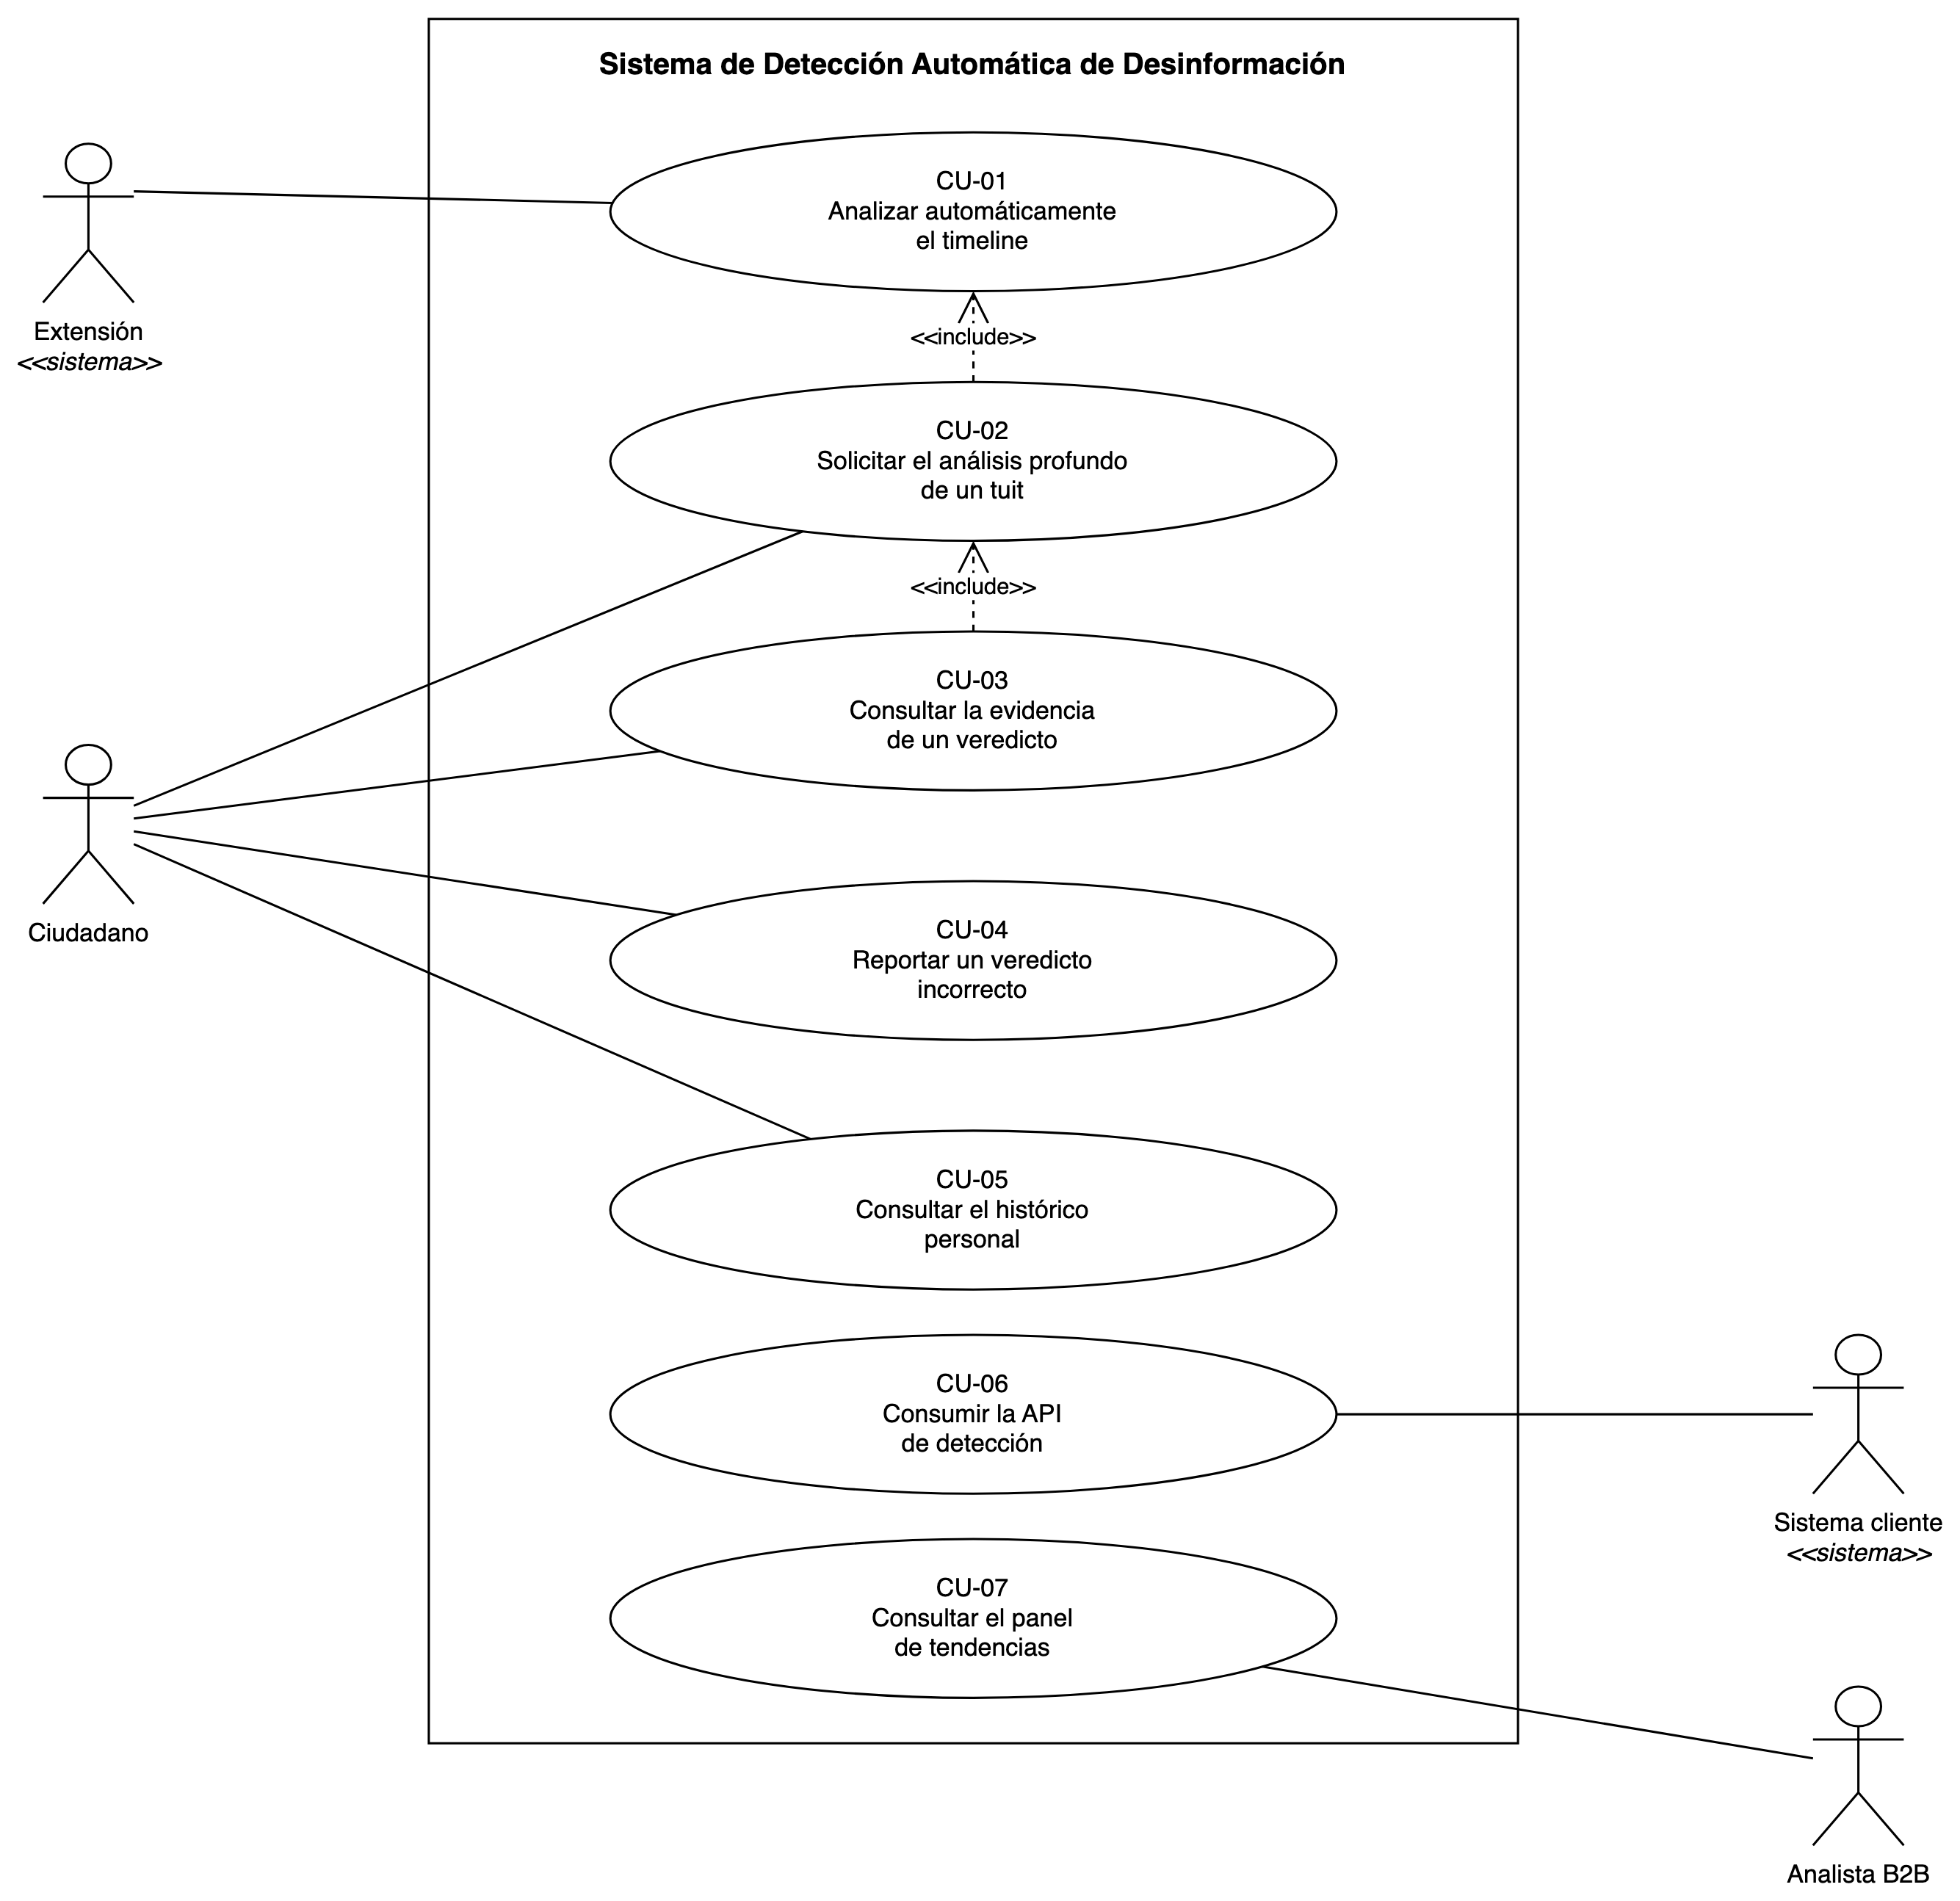
\includegraphics[width=0.92\linewidth]{chapters/figures/casos-de-uso}
  \caption{Diagrama de casos de uso del sistema. Las relaciones de inclusión indican que el análisis profundo presupone la detección previa de la publicación y que la consulta de evidencia presupone un análisis completo. Fuente: elaboración propia.}
  \label{fig:casos-de-uso}
\end{figure}

La Tabla~\ref{tab:trazabilidad-cu} resume los siete casos de uso con su actor principal y los requerimientos funcionales que realiza. Las fichas completas, con el flujo de eventos, los flujos alternativos y las condiciones previas y posteriores de cada caso, se presentan en el Anexo~\ref{anexo:casos-uso}. La relación entre casos de uso y requerimientos cumple además una segunda función: opera como regla de corte para el modelo de datos que se desarrolla en la Sección~\ref{sec:modelo-datos}, donde toda entidad debe resultar trazable hasta un requerimiento de esta lista.

\begin{table}[t]
  \centering
  \small
  \caption{Casos de uso del sistema, con su actor principal y los requerimientos funcionales que realizan. Fuente: elaboración propia.}
  \label{tab:trazabilidad-cu}
  \begin{tabular}{l p{5.4cm} p{2.2cm} p{4.4cm}}
    \hline
    \textbf{Código} & \textbf{Nombre} & \textbf{Actor} & \textbf{Requerimientos} \\
    \hline
    CU-01 & Analizar automáticamente la línea de tiempo & Extensión & RF-01, RF-02, RF-06, RF-07, RF-08, RF-16 \\
    CU-02 & Solicitar el análisis profundo de una publicación & Ciudadano & RF-03, RF-04, RF-05, RF-06, RF-08, RF-09, RF-16 \\
    CU-03 & Consultar la evidencia de un veredicto & Ciudadano & RF-09 \\
    CU-04 & Informar un veredicto incorrecto & Ciudadano & RF-11 \\
    CU-05 & Consultar el histórico personal & Ciudadano & RF-10 \\
    CU-06 & Consumir la API & Sistema cliente & RF-13, RF-15 \\
    CU-07 & Consultar el panel de tendencias & Analista & RF-13, RF-14, RF-15 \\
    \hline
  \end{tabular}
\end{table}

RF-12 es el único requerimiento sin caso de uso asociado, circunstancia que responde a su naturaleza y no a una omisión: se trata de un requerimiento de superficie y no de flujo. Los dos textos que prescribe permanecen visibles en la interfaz de la extensión y en el panel web, y ningún caso de uso los persigue como objetivo. Su ausencia en la matriz no lo vuelve opcional, razón por la cual conserva prioridad imprescindible.

\subsection{Producto}
\label{sec:producto}

En esta subsección se presenta la identidad pública del producto, que se denomina \textbf{Factum}. Se describen el estilo (paleta, tipografía y tono de voz), el logotipo, la misión y la visión. Las elecciones se fundamentan en la gestión de marca (\textit{branding}), cuyo objeto es la identidad de marca: el conjunto de nombre, símbolo, color, tipografía y voz que vuelve reconocible a un producto y que debe mantenerse coherente en todos los puntos de contacto con el usuario \parencite{Wheeler2017}. Un producto que se pronuncia sobre lo que otros publican le agrega a esa coherencia una condición propia, porque ningún elemento de la marca puede sugerir que el producto toma partido. La encuesta identifica ese riesgo como central: la ausencia de sesgo político encabeza los atributos de confianza con un 84,1\,\% (Figura~\ref{fig:encuesta-drivers}).

\textit{Factum} es un término latino que significa \enquote{hecho} o \enquote{lo que fue hecho}, participio de \textit{facere}. Para evaluarlo se aplicaron los seis criterios que Keller propone para elegir elementos de marca: que resulten memorables, significativos, agradables, transferibles, adaptables y protegibles \parencite{Keller2013}. El nombre tiene dos sílabas y se lee igual en español y en inglés. Sugiere la función del sistema, que contrasta una afirmación con lo que efectivamente consta en una fuente, aunque no la describe de forma literal. Su registro es el de las actas y los expedientes, es decir, el de un documento que se puede abrir y consultar, que es lo que el producto ofrece cuando acompaña cada veredicto con la evidencia enlazada. No depende de X ni de una tecnología determinada, de modo que sirve tanto para la extensión gratuita como para la API y el panel de tendencias, y resistiría un cambio de plataforma o de modelo. Tampoco recurre a \enquote{verdad}, \enquote{falso} ni al vocabulario de las \textit{fake news}, y nombra lo que se afirmó sin aludir a quién lo publicó. El criterio de protección fue el que descartó al primer candidato, \enquote{Trama}, que ya se encontraba registrado como marca en el Instituto Nacional de la Propiedad Industrial (INPI).

\subsubsection{Estilo}

El estilo se deriva de la personalidad de marca, definida como el conjunto de características humanas que el público asocia a una marca \parencite{Aaker1996}. Factum se ubica en las dimensiones de competencia y sinceridad; la de emoción corresponde a productos cuyo valor reside en la novedad o el entretenimiento. La paleta, la tipografía y el tono se eligieron a partir de esa personalidad.

\textit{Paleta.} La Tabla~\ref{tab:paleta} presenta los colores de marca. El color principal es un azul tinta, que remite a la tinta y al papel impreso y que no tiene asociación partidaria en Argentina. Se descartaron dos alternativas: el celeste, porque carga identidad nacional y se confunde con el azul de X, y el verde y el rojo, porque dentro de la interfaz ya expresan el estado del veredicto (Figura~\ref{fig:badge}). Una marca verde diría \enquote{verificado} en cada lugar donde aparece, y una roja diría \enquote{falso}. Por ese motivo los colores de estado quedan fuera de la marca: la marca firma el análisis y el color de estado comunica su resultado, de modo que la firma no se lee como un juicio. El azul tinta alcanza una relación de contraste de 13,3:1 sobre blanco, y los neutros se eligieron para que el texto de cuerpo y los epígrafes superen el mínimo de 4,5:1.

\begin{table}[t]
  \centering
  \small
  \caption{Colores de marca de Factum. Los colores de estado del veredicto no forman parte de la marca. Fuente: elaboración propia.}
  \label{tab:paleta}
  \begin{tabular}{c l l p{7.2cm}}
    \hline
     & \textbf{Nombre} & \textbf{Código} & \textbf{Uso} \\
    \hline
    \textcolor[HTML]{1B2F52}{\rule{1.2em}{1.2em}} & Azul tinta & \#1B2F52 & Color principal: logotipo, títulos y fondo del ícono \\
    \textcolor[HTML]{6F8FC0}{\rule{1.2em}{1.2em}} & Azul evidencia & \#6F8FC0 & Mitad de la evidencia en el logotipo y acentos gráficos \\
    \textcolor[HTML]{8FAEDB}{\rule{1.2em}{1.2em}} & Azul evidencia claro & \#8FAEDB & Mitad de la evidencia sobre fondo oscuro \\
    \fcolorbox[HTML]{D9DCE1}{F7F6F2}{\rule{0pt}{1em}\hspace{1em}} & Papel & \#F7F6F2 & Fondo de presentaciones y piezas impresas \\
    \textcolor[HTML]{2A2E35}{\rule{1.2em}{1.2em}} & Grafito & \#2A2E35 & Texto de cuerpo \\
    \textcolor[HTML]{6B7280}{\rule{1.2em}{1.2em}} & Pizarra & \#6B7280 & Texto secundario y epígrafes \\
    \textcolor[HTML]{D9DCE1}{\rule{1.2em}{1.2em}} & Línea & \#D9DCE1 & Filetes y separadores \\
    \hline
  \end{tabular}
\end{table}

\textit{Tipografía.} La familia tipográfica combina Source Serif 4, para la palabra del logotipo y los títulos, con Source Sans 3, para el texto de las presentaciones y las piezas de comunicación. Ambas son de Adobe, se distribuyen con licencia libre (\textit{SIL Open Font License}) y cubren el español completo. La serif refuerza el registro documental del nombre, porque es la letra de los diarios y los boletines oficiales, que son las mismas fuentes contra las que el sistema contrasta. La sans comparte proporciones con la serif y se lee mejor en pantalla y en proyección. La interfaz de la extensión no adopta estas fuentes y conserva las del sistema que utiliza X: la extensión se presenta dentro de una interfaz ajena, y su identidad se expresa a través del logotipo y del veredicto.

\textit{Tono de voz.} El tono es sobrio: frases cortas, sin exclamaciones ni adjetivos de alarma. Se escribe en voseo, el registro rioplatense del usuario, porque el tuteo o el usted se leerían como una traducción. El sujeto de cada enunciado es la afirmación o la fuente y nunca la cuenta que publicó; el producto dice, por ejemplo, \enquote{esta afirmación contradice lo publicado por el INDEC}, y no \enquote{este usuario miente}. La incertidumbre queda a la vista: se informan probabilidades y fuentes, y cuando no hay evidencia se lo declara. El lema (\textit{tagline}) resume el posicionamiento en una frase: \enquote{Cada afirmación, con su evidencia}. Nombra las dos mitades del logotipo en el orden en que se leen, evita prometer lo que el sistema no hace y, mediante \enquote{cada}, expresa que cualquier afirmación recibe el mismo tratamiento, sea cual fuere su signo político.

\subsubsection{Logo}

El logotipo de Factum, que presenta la Figura~\ref{fig:logo}, combina un símbolo y la palabra. El símbolo es un círculo dividido por un eje vertical. La mitad izquierda representa la afirmación y la derecha, la evidencia, mientras que el eje funciona como el fiel de una balanza, la aguja que indica el equilibrio entre los platillos. Las dos mitades tienen el mismo tamaño y ninguna pesa más que la otra, y esa simetría comunica la neutralidad. Ambas mitades usan dos tonos del mismo azul, porque afirmación y evidencia forman parte de una misma operación y ninguna de las dos es la \enquote{correcta}.

\begin{figure}[t]
  \centering
  
\includegraphics[width=0.42\linewidth]{images/factum-logo}
  \hspace{0.06\linewidth}
  
\includegraphics[width=0.42\linewidth]{images/factum-logo-mono}
  \caption{Logotipo de Factum. A la izquierda, la versión en color; a la derecha, la versión monocroma, en la que la mitad de la evidencia pasa a contorno para distinguirse sin color. Fuente: elaboración propia.}
  \label{fig:logo}
\end{figure}

El dibujo literal de una balanza de platillos se descartó por dos motivos. A 16 píxeles, el menor de los tamaños de ícono que pide la tienda de extensiones, se convierte en una mancha. Además, es el emblema habitual de los estudios jurídicos, lo que llevaría a leer el producto como un tribunal que condena. El círculo partido abstrae la misma idea con una geometría mínima, de dos semicírculos y una barra, sin degradados ni detalles que se pierdan al reducirlo. Ese símbolo, además, ya era la marca de atribución que la extensión muestra junto a cada indicador; el logotipo le agrega el fiel y conserva la continuidad que la identidad de marca exige entre los puntos de contacto \parencite{Wheeler2017}. La palabra se compone en Source Serif 4 seminegrita. La versión monocroma se destina a impresión y a fondos de un solo color.

\subsubsection{Misión}

La misión de Factum consiste en poner a disposición de cualquier ciudadano argentino una herramienta automática y verificable que le permita identificar contenido desinformativo mientras consume información digital, y construir sobre esa base un registro sistemático de la circulación de desinformación en el país.

\subsubsection{Visión}

La visión de Factum consiste en constituirse en la referencia del ecosistema informativo argentino sobre esa materia: la fuente que medios, verificadores, investigadores y organismos públicos consultan cuando necesitan conocer qué contenido desinformativo circula, con qué intensidad y sobre qué temas.

\subsection{Interfaz de usuario}
\label{sec:interfaz}

El diseño de la interfaz se construyó mediante prototipos en HTML y CSS reales, en lugar de recurrir a una herramienta de diseño gráfico. La decisión responde a un criterio de continuidad: el marcado de estos prototipos es la base de la implementación, de manera que el indicador que se superpone sobre la publicación en el producto es el mismo componente y no una reconstrucción posterior. Las capturas que se presentan a continuación se generaron mediante un navegador en modo automatizado a doble resolución.

El contenido de las cuatro pantallas es ficticio. Las cuentas, las publicaciones, los titulares y las verificaciones fueron construidos sobre temas argentinos verosímiles, y cada pantalla incorpora un rótulo que lo advierte. La decisión es necesaria por coherencia con el análisis desarrollado en la Sección~\ref{sec:legal}: un documento que señalara a una cuenta identificable como origen de contenido desinformativo contradiría su propio apartado sobre delitos contra el honor.

Las cuatro pantallas no cumplen una función ilustrativa. Cada una materializa una decisión de diseño que sostiene un requerimiento, y esas decisiones se explicitan a continuación de cada figura.

\begin{figure}[t]
  \centering
  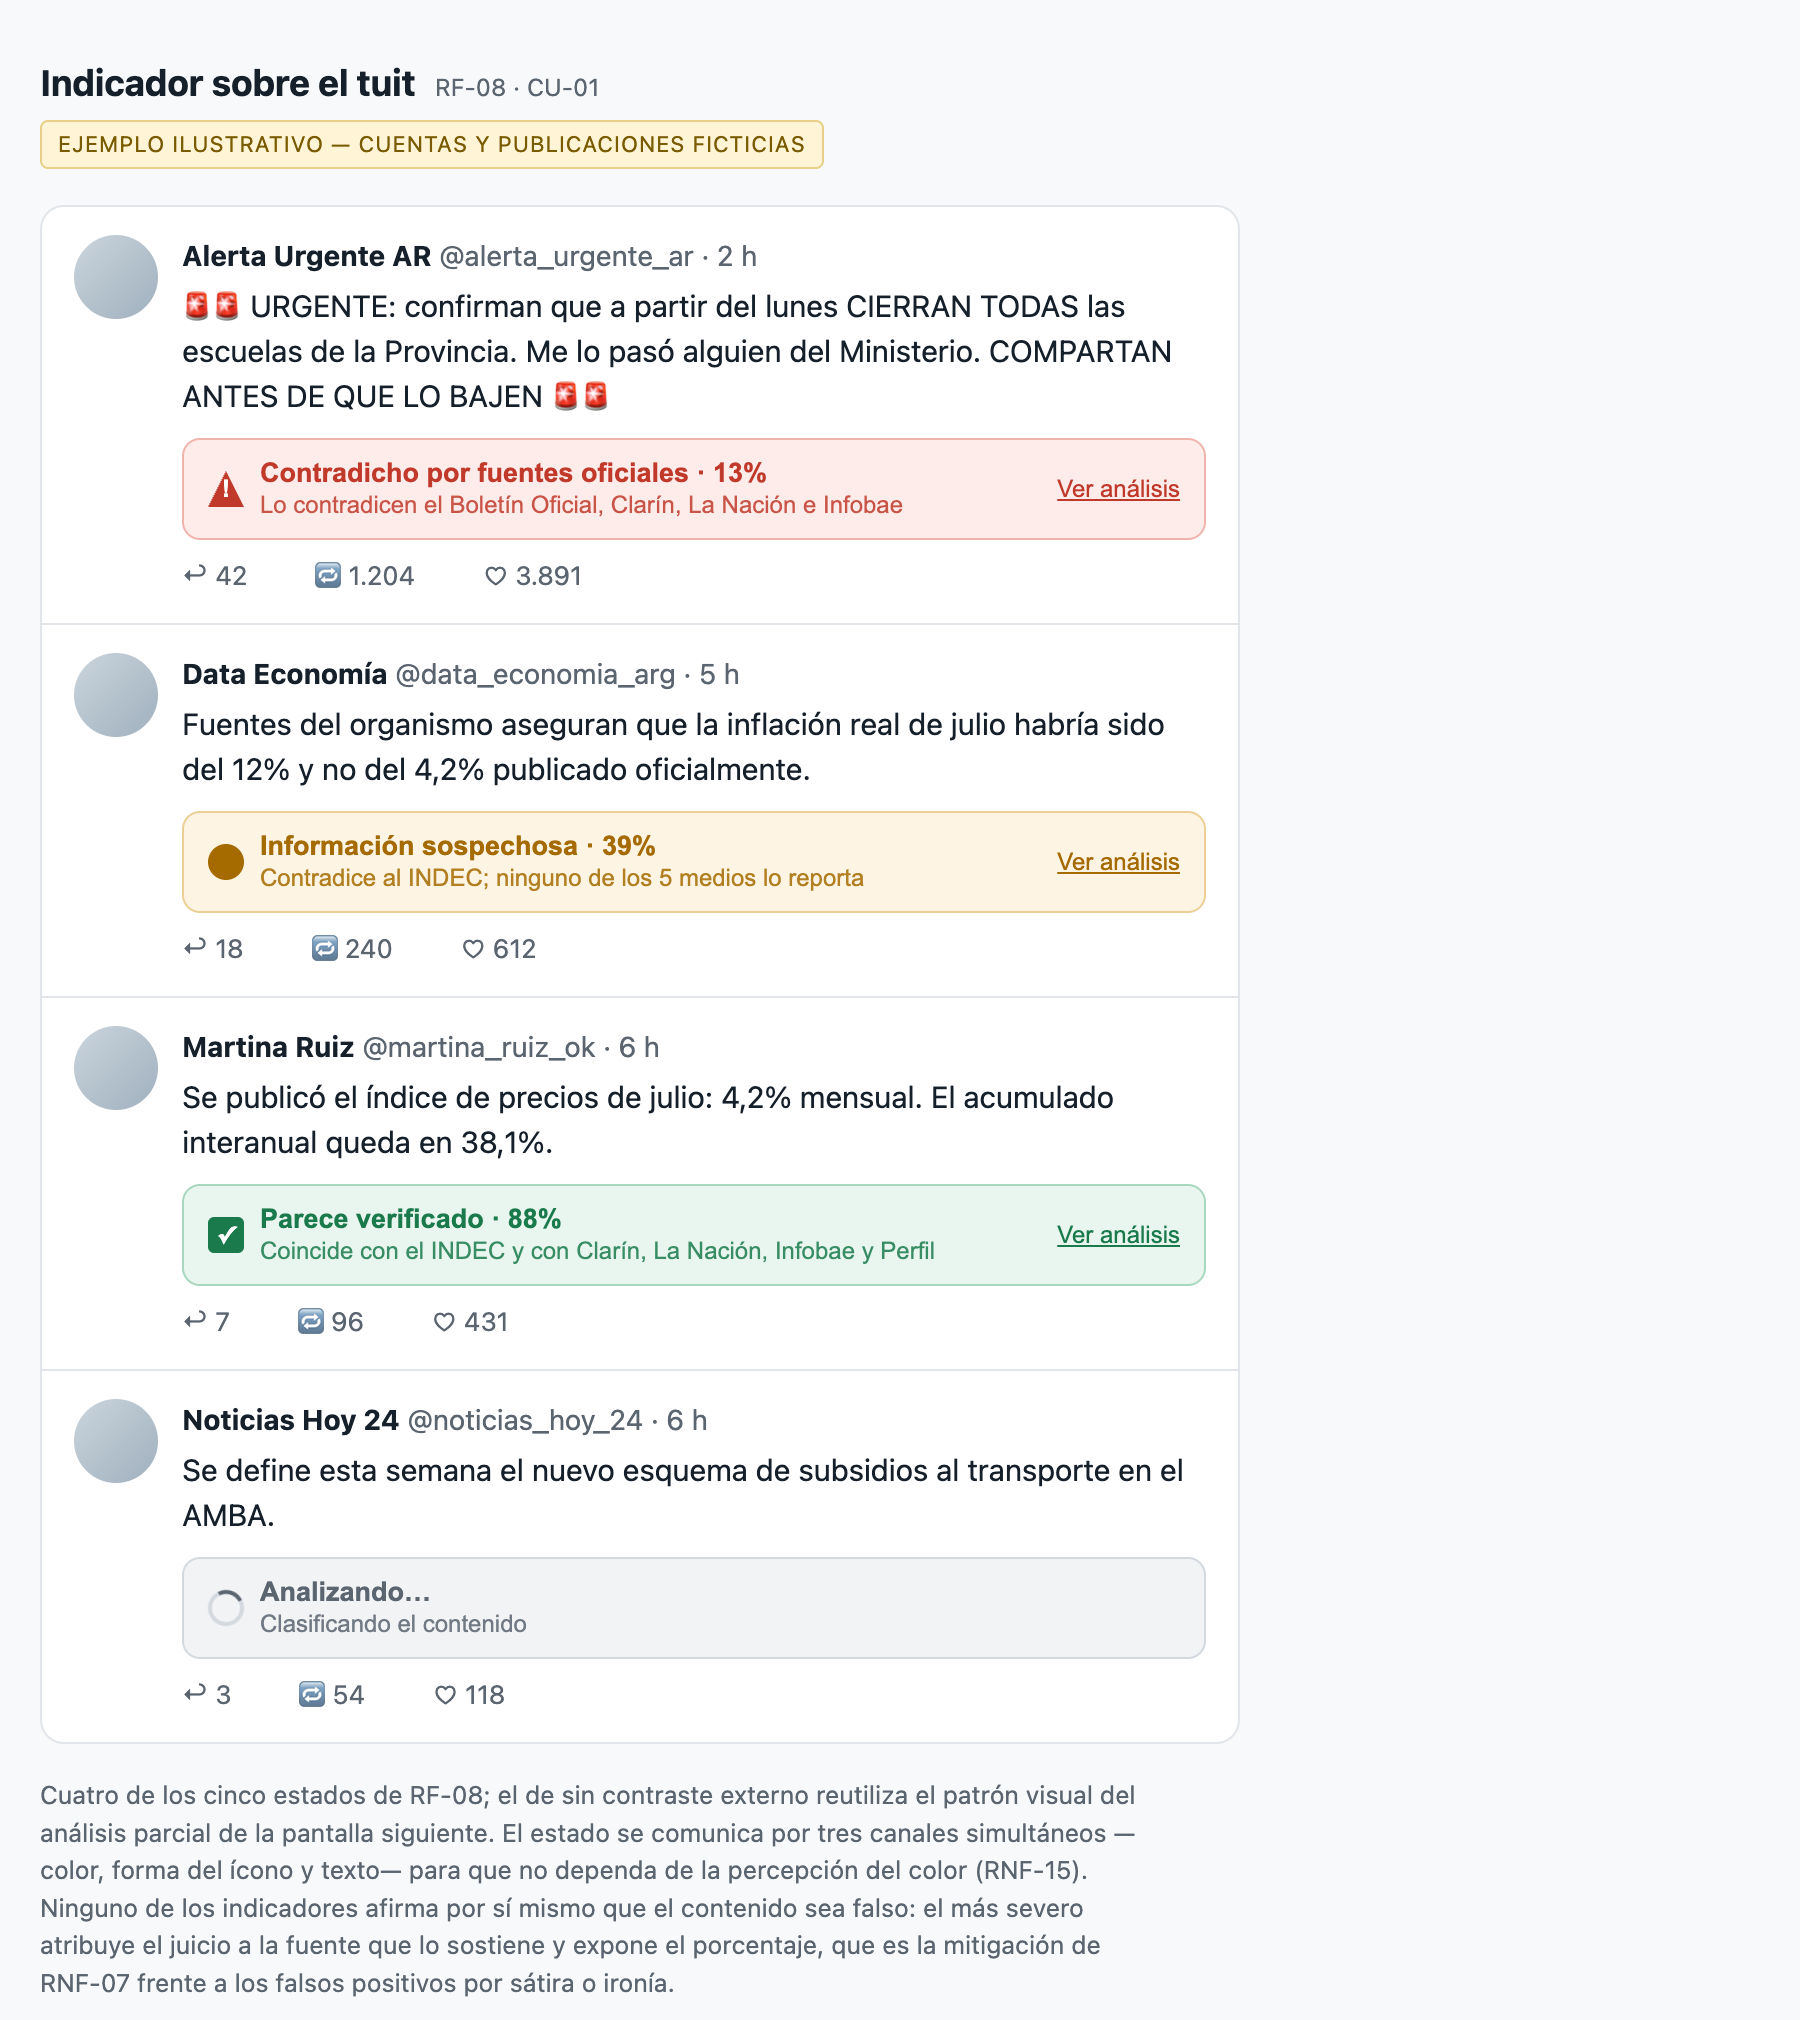
\includegraphics[width=0.72\linewidth]{chapters/figures/badge}
  \caption{Indicador superpuesto sobre las publicaciones de la línea de tiempo, en sus cuatro estados visibles. El contenido es ficticio. Fuente: elaboración propia.}
  \label{fig:badge}
\end{figure}

La Figura~\ref{fig:badge} presenta el indicador que realiza RF-08, la pantalla de mayor relevancia del producto por tratarse de la única que el usuario percibe sin haber formulado solicitud alguna. Dos decisiones de diseño la gobiernan. En primer lugar, el estado se comunica de forma simultánea por tres canales (color, forma del ícono y texto) de modo que una persona que no distingue el rojo del verde lee el enunciado y percibe un triángulo en lugar de una marca de verificación; ese redundancia es lo que vuelve cumplible RNF-15. En segundo lugar, ningún indicador afirma por cuenta propia que el contenido resulte falso: el nivel más severo atribuye el juicio a las fuentes que lo sostienen. Esa formulación traduce RNF-07 al plano visual y es la que permite encuadrar el enunciado en la eximente de atribución fiel del artículo 113 del Código Penal, según se desarrolla en la Sección~\ref{sec:legal}. El indicador incorpora además una línea que nombra las fuentes en lugar de contabilizarlas, con lo que anticipa la evidencia sin obligar a abrir el detalle y permite al usuario ponderar la señal en lugar de confiar en ella.

\begin{figure}[t]
  \centering
  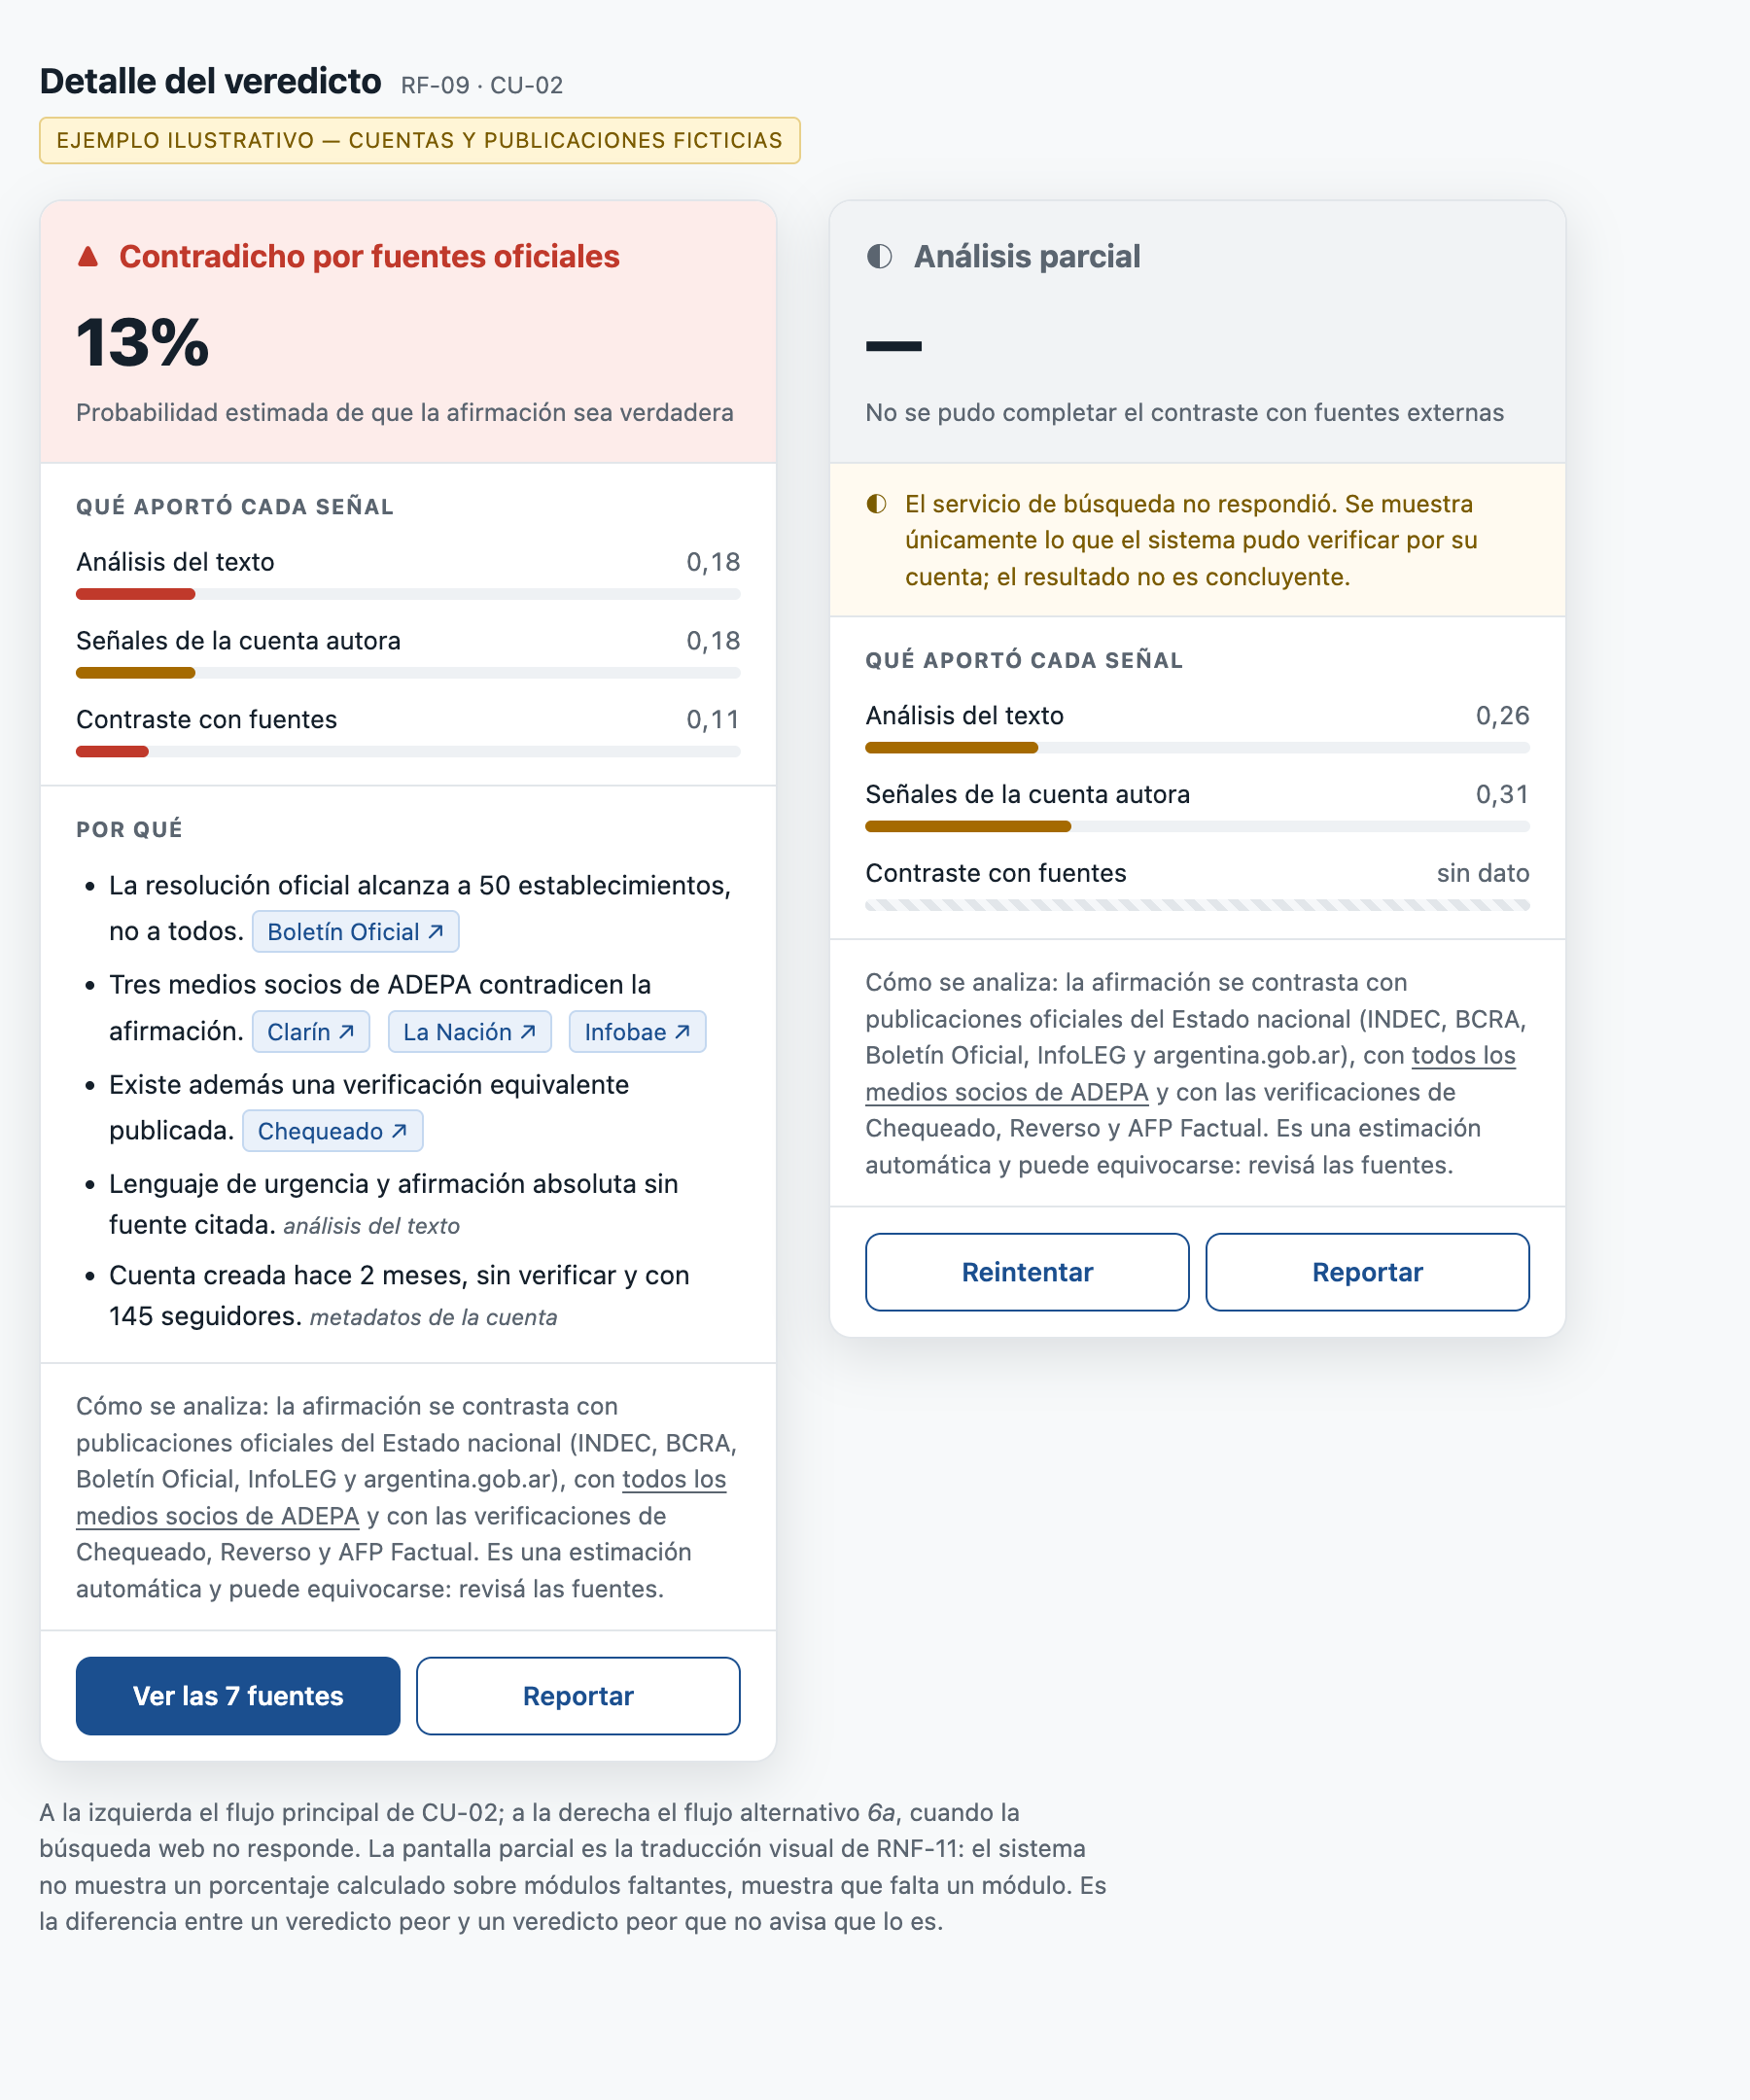
\includegraphics[width=0.85\linewidth]{chapters/figures/popup}
  \caption{Detalle del veredicto. A la izquierda, el flujo principal con el desglose de los tres puntajes parciales; a la derecha, el flujo degradado cuando un módulo de contraste no respondió. El contenido es ficticio. Fuente: elaboración propia.}
  \label{fig:popup}
\end{figure}

La Figura~\ref{fig:popup} realiza RF-09 y presenta dos estados en una misma captura. El estado principal exhibe el puntaje final, expresado como la probabilidad estimada de que la afirmación sea verdadera, y el desglose de los tres puntajes parciales, y ese desglose es lo que vuelve auditable el resultado: permite advertir que el análisis del texto obtuvo un valor determinado pero que el veredicto se desplazó por efecto del contraste con fuentes externas. Cada razón incorpora el enlace de la fuente que la respalda y las razones se ordenan según la jerarquía de evidencia; las dos señales que el sistema produce por cuenta propia, el análisis del texto y las señales de la cuenta, se distinguen mediante una etiqueta neutra en lugar de un enlace, dado que no existe documento externo que exhibir. Esa distinción visual separa lo que el sistema encontró de lo que el sistema infirió, y solo lo primero admite verificación por parte del usuario.

El estado de la derecha corresponde al flujo degradado y traduce RNF-11. No presenta porcentaje sino un guion, la barra del módulo ausente aparece rayada y su etiqueta declara la falta de dato. Un sistema que calculara el promedio ponderado con un módulo caído devolvería un número con la misma apariencia de confiabilidad que los demás sin poseerla; la decisión de diseño consiste en exhibir la ausencia como ausencia en lugar de disimularla mediante aritmética.

\begin{figure}[t]
  \centering
  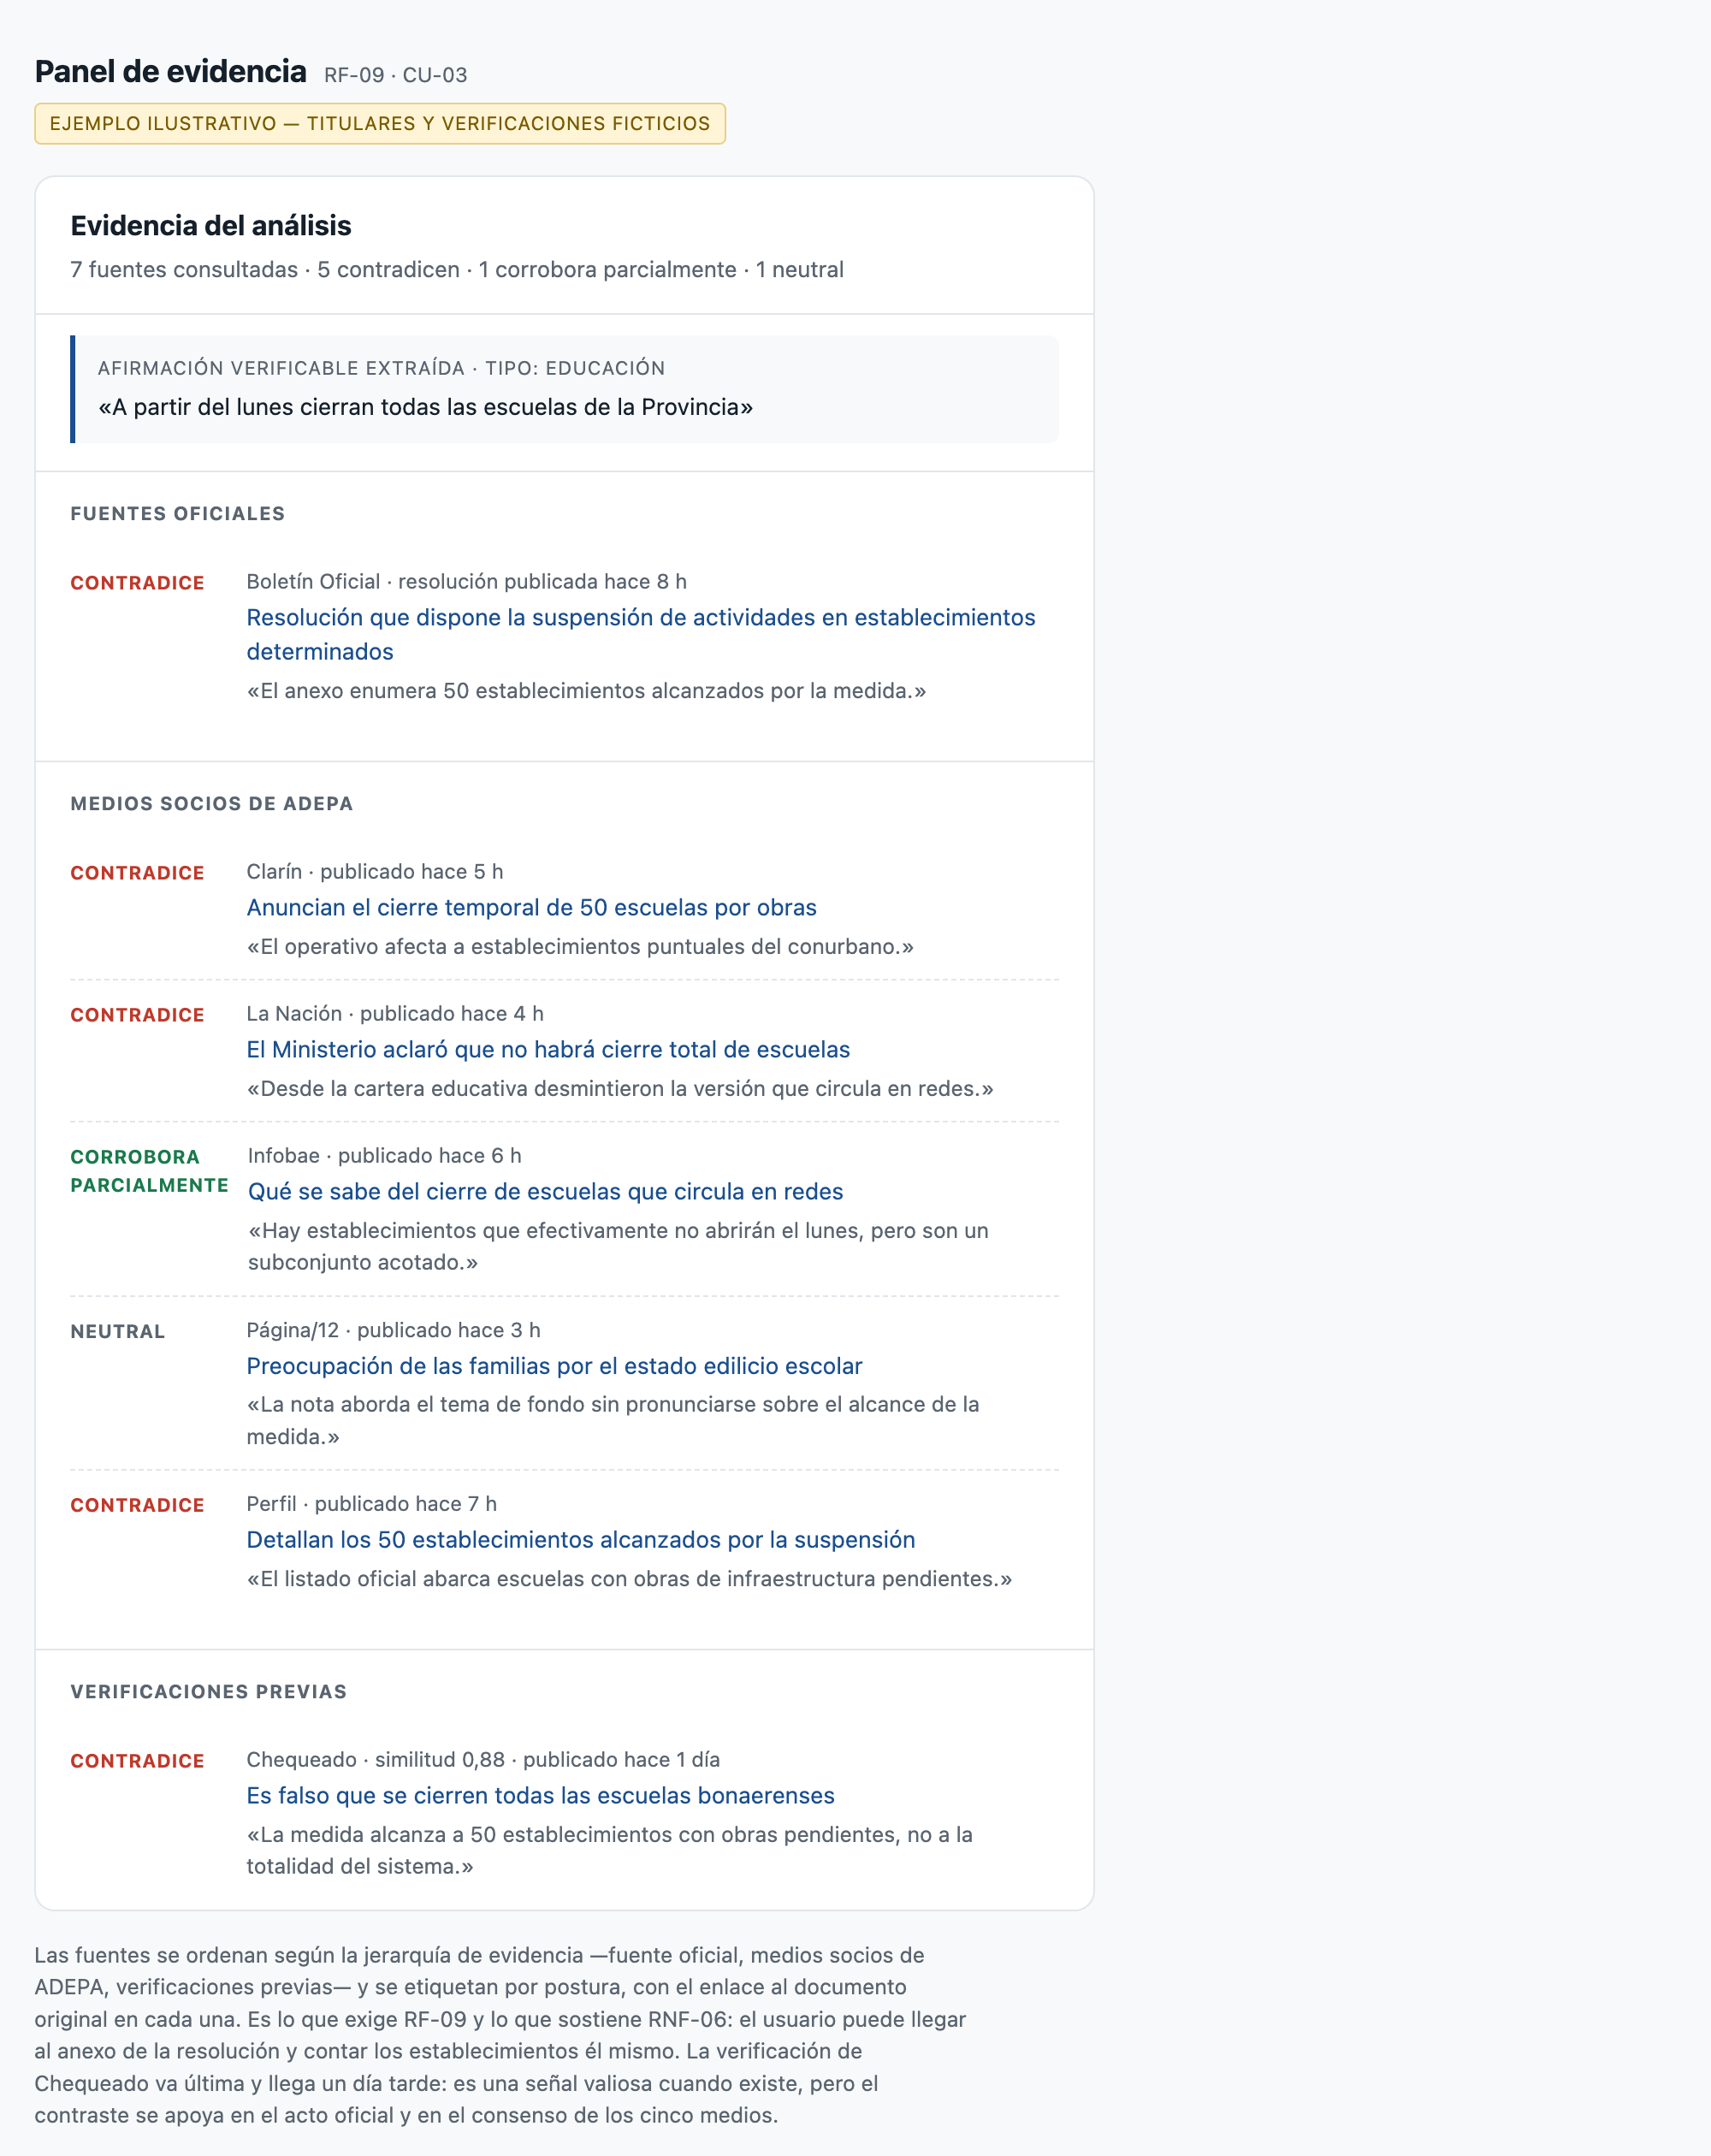
\includegraphics[width=0.92\linewidth]{chapters/figures/evidencia}
  \caption{Panel de evidencia con las fuentes consultadas, ordenadas según la jerarquía de evidencia y etiquetadas por postura. El contenido es ficticio. Fuente: elaboración propia.}
  \label{fig:evidencia}
\end{figure}

El panel de la Figura~\ref{fig:evidencia} realiza RF-09 en su segunda mitad y presenta las fuentes consultadas agrupadas por tipo y etiquetadas según su postura. El orden de los grupos es la decisión de fondo de esta pantalla. Los medios de referencia operan como columna vertebral del contraste y no como complemento, dado que cubren cualquier tema de relevancia pública en cuestión de horas y aportan consenso, señal que una fuente aislada no puede proporcionar. El detalle incorpora además una aclaración que declara contra qué fuentes se contrasta la afirmación y enlaza al padrón público del que provienen los medios, de modo que el usuario pueda auditar el criterio de inclusión y no solo el resultado. La verificación profesional aparece en último lugar y con su fecha visible, circunstancia que ilustra el problema que el trabajo aborda: la desinformación cuya detección interesa es, por definición, aquella que todavía nadie verificó.

En el encabezado se presenta la afirmación verificable que el sistema extrajo de la publicación, junto con su tipo. El detalle no es menor: evidencia que el sistema compara una afirmación acotada y no la publicación completa contra la totalidad de la web, y explicita cuál. Si la extracción resultó incorrecta, el usuario lo advierte en la primera línea y comprende el motivo por el cual el veredicto no lo convence. La pantalla incorpora de forma deliberada una fuente que corrobora parcialmente y otra neutral: un panel donde la totalidad de las fuentes apunta en la misma dirección constituiría un panel de confirmación y no de evidencia.

\begin{figure}[t]
  \centering
  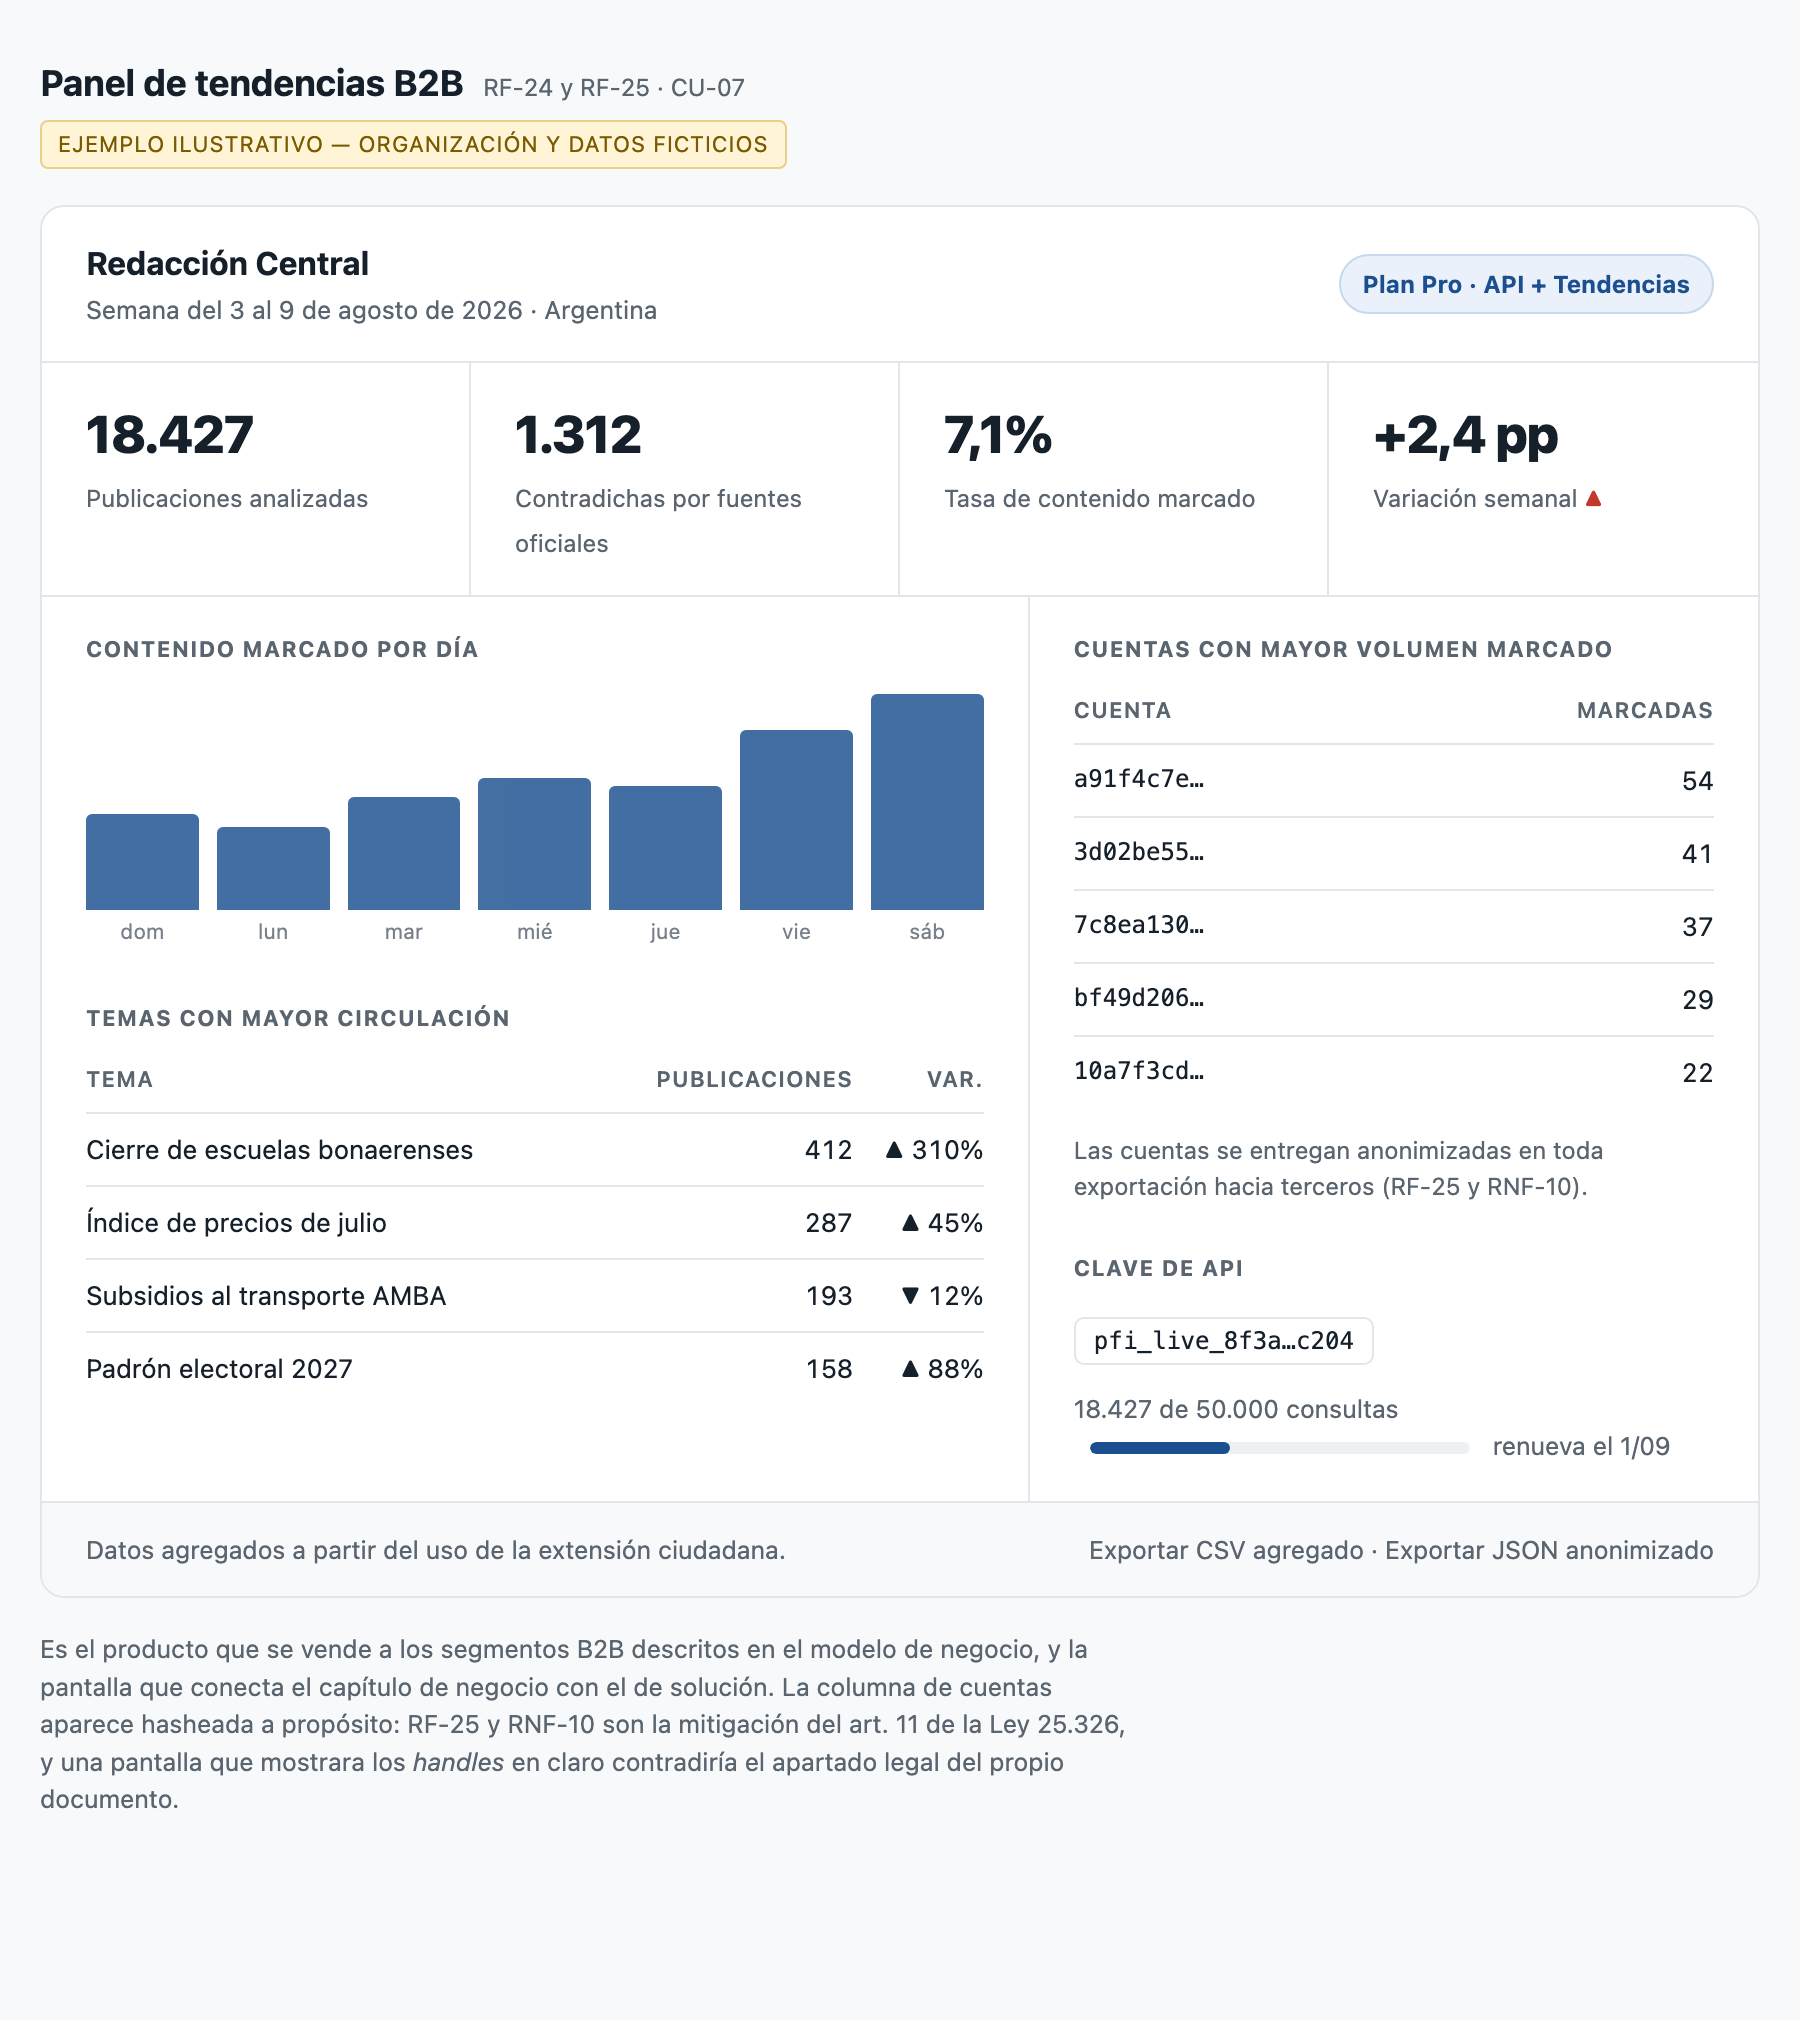
\includegraphics[width=0.92\linewidth]{chapters/figures/dashboard}
  \caption{Panel de tendencias para organizaciones cliente. La columna de cuentas se presenta seudonimizada. El contenido es ficticio. Fuente: elaboración propia.}
  \label{fig:dashboard}
\end{figure}

La Figura~\ref{fig:dashboard} realiza RF-14 y RF-15, y es el producto que se comercializa a los segmentos descritos en la Sección~\ref{sec:negocio}. Presenta el volumen analizado, la proporción de contenido marcado con su variación, la evolución diaria, los temas de mayor circulación, las cuentas de mayor volumen y el consumo de la clave contra la cuota del plan. La columna de cuentas aparece seudonimizada de forma deliberada: RF-15 y RNF-10 exigen que toda entrega hacia terceros se realice de forma agregada o con la cuenta autora anonimizada, puesto que la comunicación del conjunto de datos con los nombres de usuario en claro constituiría una cesión de datos personales en los términos del artículo 11 de la Ley 25.326. Un prototipo que exhibiera esos nombres en esta pantalla contradiría el apartado legal del propio trabajo.

Tres pantallas quedan fuera de este conjunto: la instalación y configuración de la extensión, el formulario de informe de veredicto incorrecto y los estados de error de conectividad. Las tres corresponden a requerimientos de prioridad importante o deseable y no introducen decisiones de diseño adicionales a las descritas.

\subsection{Arquitectura del sistema}
\label{sec:arquitectura}

El sistema consiste en una extensión de navegador con un servicio de análisis asociado. Se estructura en cuatro piezas desplegables (la extensión, un panel web, una API REST y una tarea programada de ingesta) a las que se suman una base de datos y un servicio de inferencia externo. Los cuatro módulos de análisis se ejecutan sobre la API.

Dos restricciones determinaron el resto de las decisiones y se enuncian antes de presentar los diagramas. La primera es que el análisis se ejecuta en dos flujos con costos muy distintos, según se describió en la Sección~\ref{sec:requerimientos}: la bifurcación atraviesa el orquestador, la caché y el recorrido completo de la información. La segunda es que la inferencia no puede ejecutarse en el mismo contenedor que la API, y el motivo responde al presupuesto y no a la memoria disponible. El plan contratado aplica un crédito mensual de uso con facturación por consumo en lugar de un techo de memoria; un contenedor con un modelo de aproximadamente 125 millones de parámetros residente consume memoria de forma continua y agota ese crédito en pocos días, mientras que la inferencia bajo demanda se factura por invocación. El techo que decide es RNF-14, y de allí que el servicio de inferencia aparezca como sistema externo y no como una biblioteca incorporada al servicio.

La descripción sigue el modelo C4, que organiza la arquitectura en niveles de detalle progresivo, y se completa con una vista del recorrido de la información y dos vistas de secuencia.

\subsubsection{Vista de contexto}

El primer nivel, que presenta la Figura~\ref{fig:c4-contexto}, ubica al sistema frente a sus usuarios y a los servicios externos de los que depende. Interactúan dos personas: el ciudadano, que emplea la extensión de forma anónima, y el analista, autenticado y perteneciente a una organización con suscripción vigente.

\begin{landscape}
\begin{figure}[t]
  \centering
  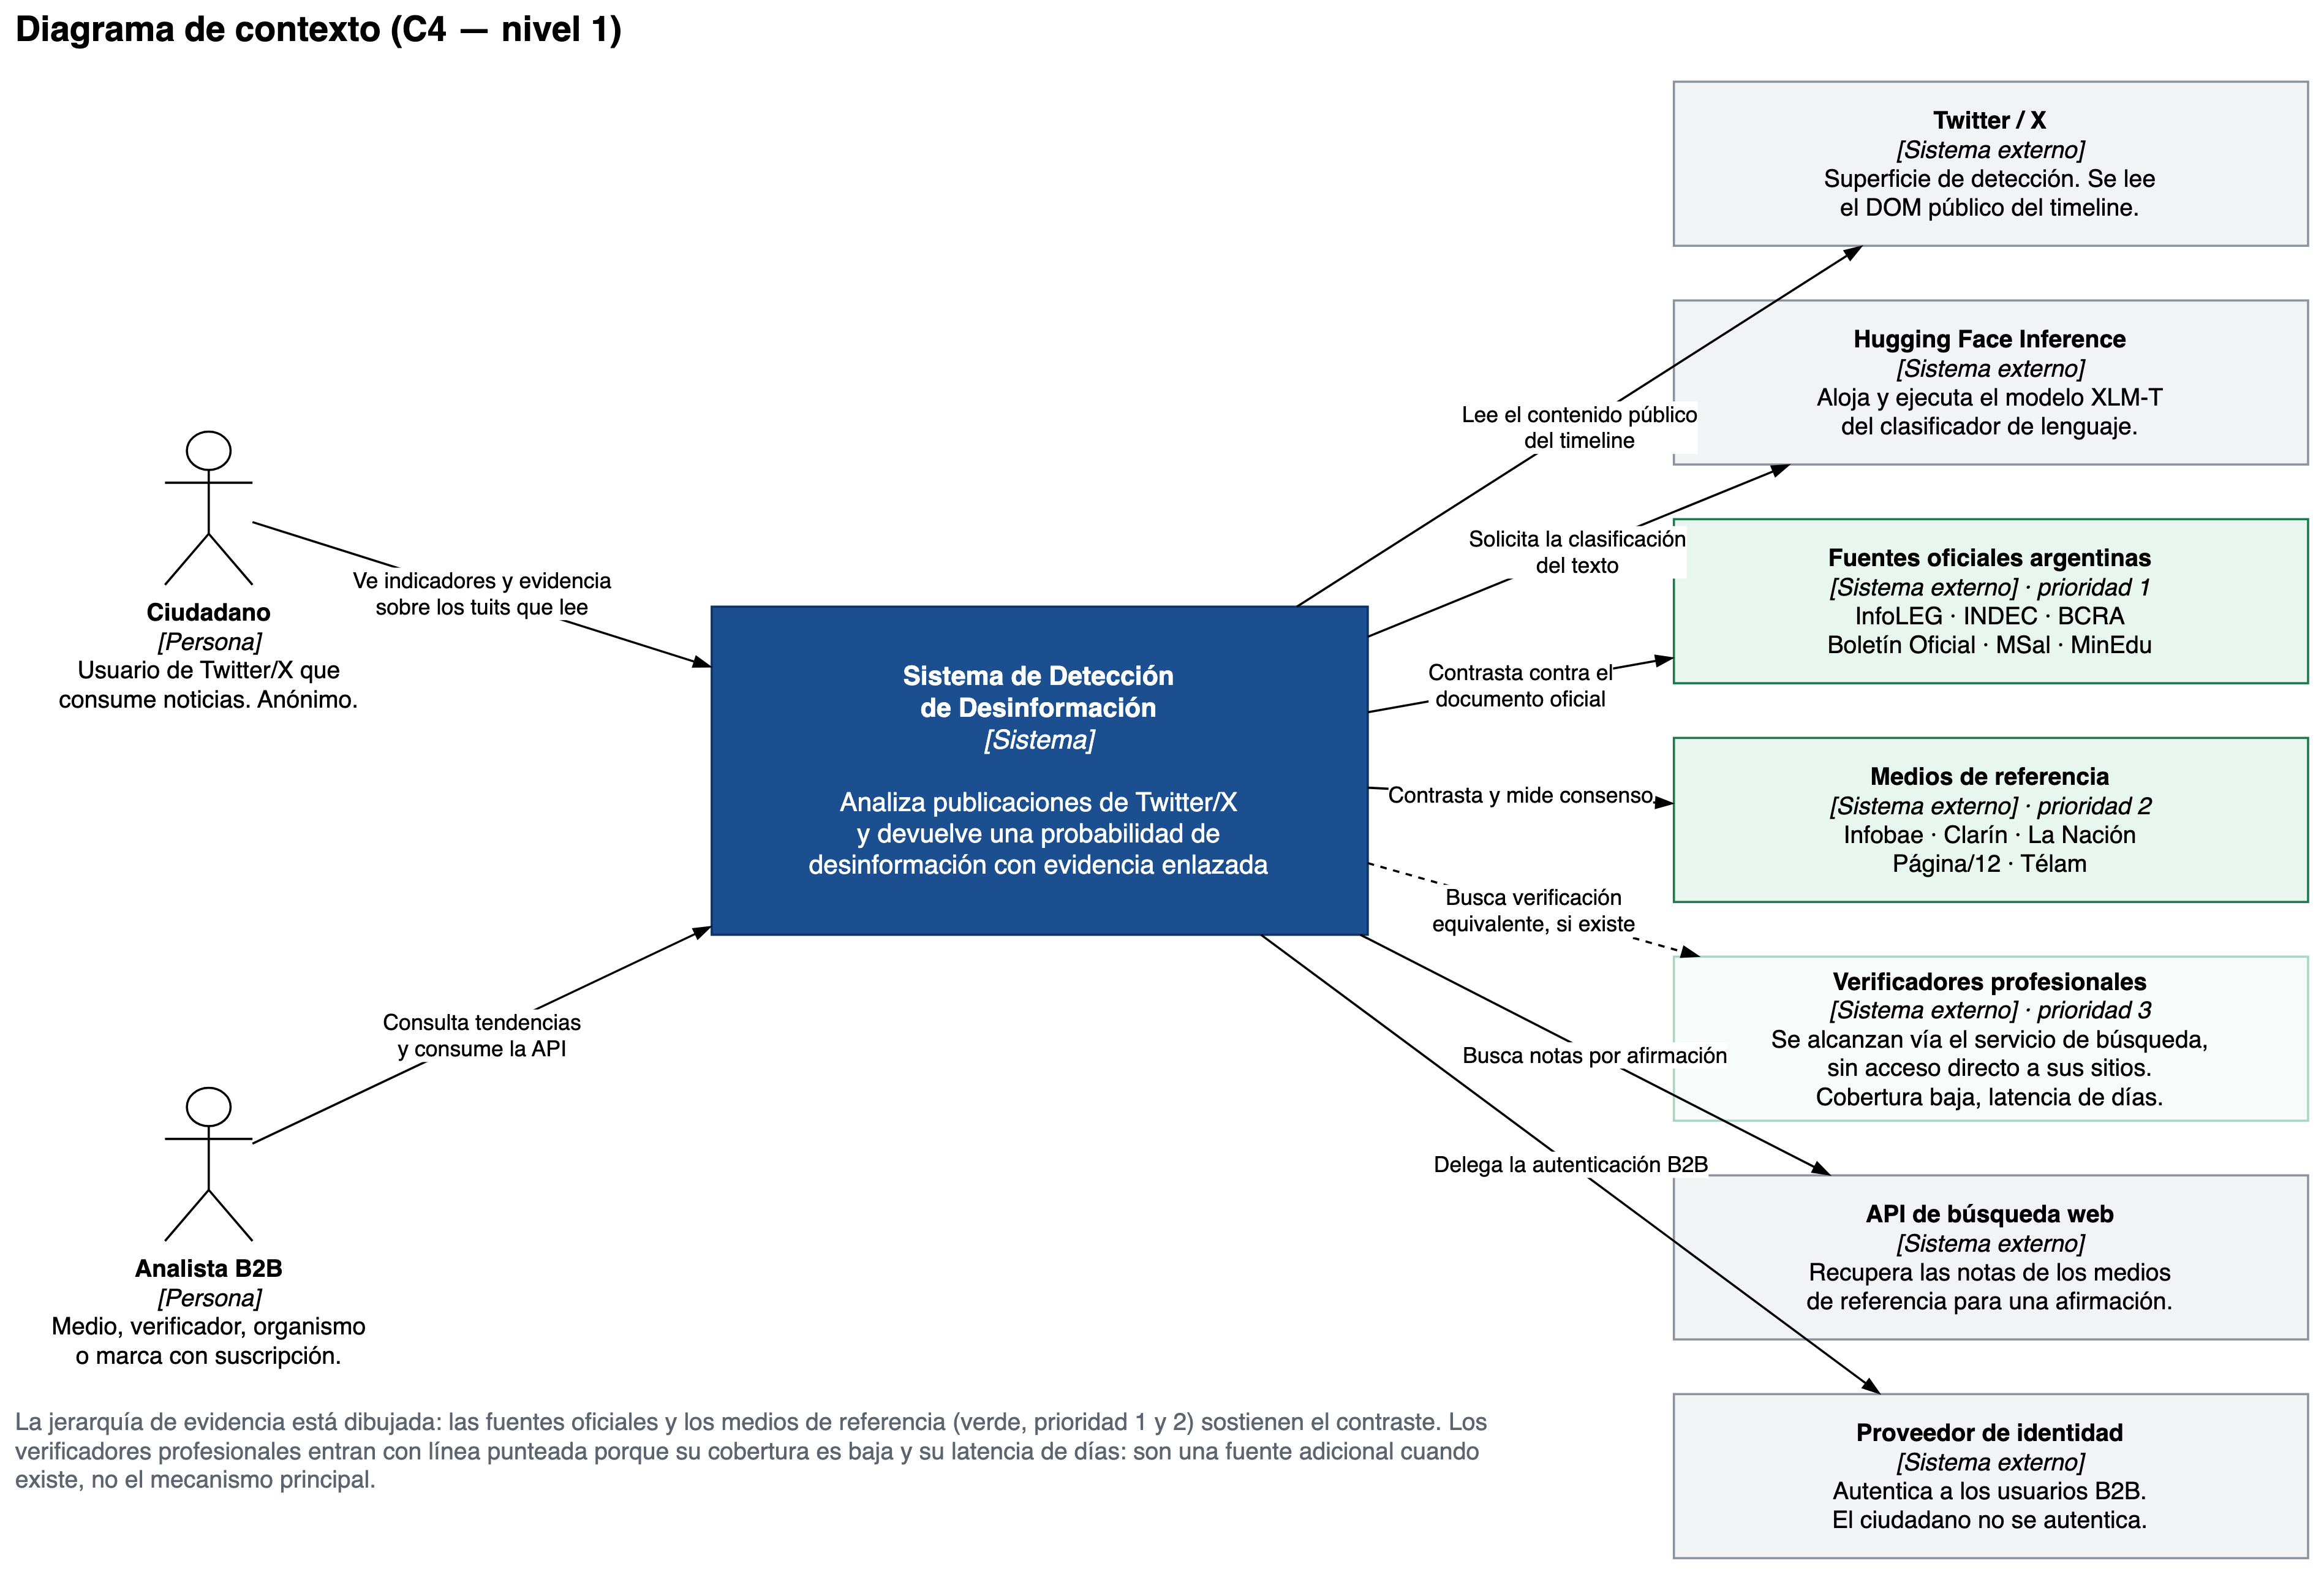
\includegraphics[width=0.95\linewidth]{chapters/figures/c4-contexto}
  \caption{Modelo C4, nivel 1: diagrama de contexto. Las fuentes oficiales y los medios de referencia se representan con línea continua; los verificadores profesionales, con línea discontinua, por su baja cobertura y su latencia de días. Fuente: elaboración propia.}
  \label{fig:c4-contexto}
\end{figure}
\end{landscape}

La dependencia de servicios externos es en sí misma un riesgo arquitectónico, y por esa razón el diagrama la expone desde el primer nivel. La Tabla~\ref{tab:dependencias} enumera cada dependencia junto con su función y con el comportamiento del sistema ante su indisponibilidad.

\begin{table}[t]
  \centering
  \small
  \caption{Dependencias externas del sistema y comportamiento previsto ante la indisponibilidad de cada una. Fuente: elaboración propia.}
  \label{tab:dependencias}
  \begin{tabular}{p{3.4cm} p{4.6cm} p{5.2cm}}
    \hline
    \textbf{Servicio externo} & \textbf{Función} & \textbf{Comportamiento ante su caída} \\
    \hline
    Red social & Superficie de detección: se lee el documento público de la línea de tiempo & No existe producto. Constituye la dependencia estructural \\
    Servicio de inferencia & Ejecuta el clasificador del primer módulo & No se presenta indicador; el flujo automático queda inactivo \\
    Fuentes oficiales & Contraste documental, prioridad 1 & Análisis parcial señalado como tal \\
    Medios de referencia & Contraste y consenso, prioridad 2 & Análisis parcial señalado como tal \\
    Verificadores profesionales & Verificación equivalente, prioridad 3 & Sin efecto: es el caso frecuente \\
    Servicio de búsqueda web & Recupera las notas de los medios para una afirmación & Se interrumpe el camino de medios del tercer módulo \\
    Proveedor de identidad & Autentica a los usuarios de organizaciones cliente & Afecta solo al panel de tendencias; el ciudadano no se autentica \\
    \hline
  \end{tabular}
\end{table}

Enunciada de este modo, RNF-11 deja de parecer una cláusula de estilo. La degradación a análisis parcial se sigue directamente de que el sistema dependa de siete servicios sobre los cuales no ejerce control alguno.

\subsubsection{Vista de contenedores}

El segundo nivel, que presenta la Figura~\ref{fig:c4-contenedores}, descompone el sistema en las unidades desplegables que lo integran y en las tecnologías con las que se construye cada una.

\begin{landscape}
\begin{figure}[t]
  \centering
  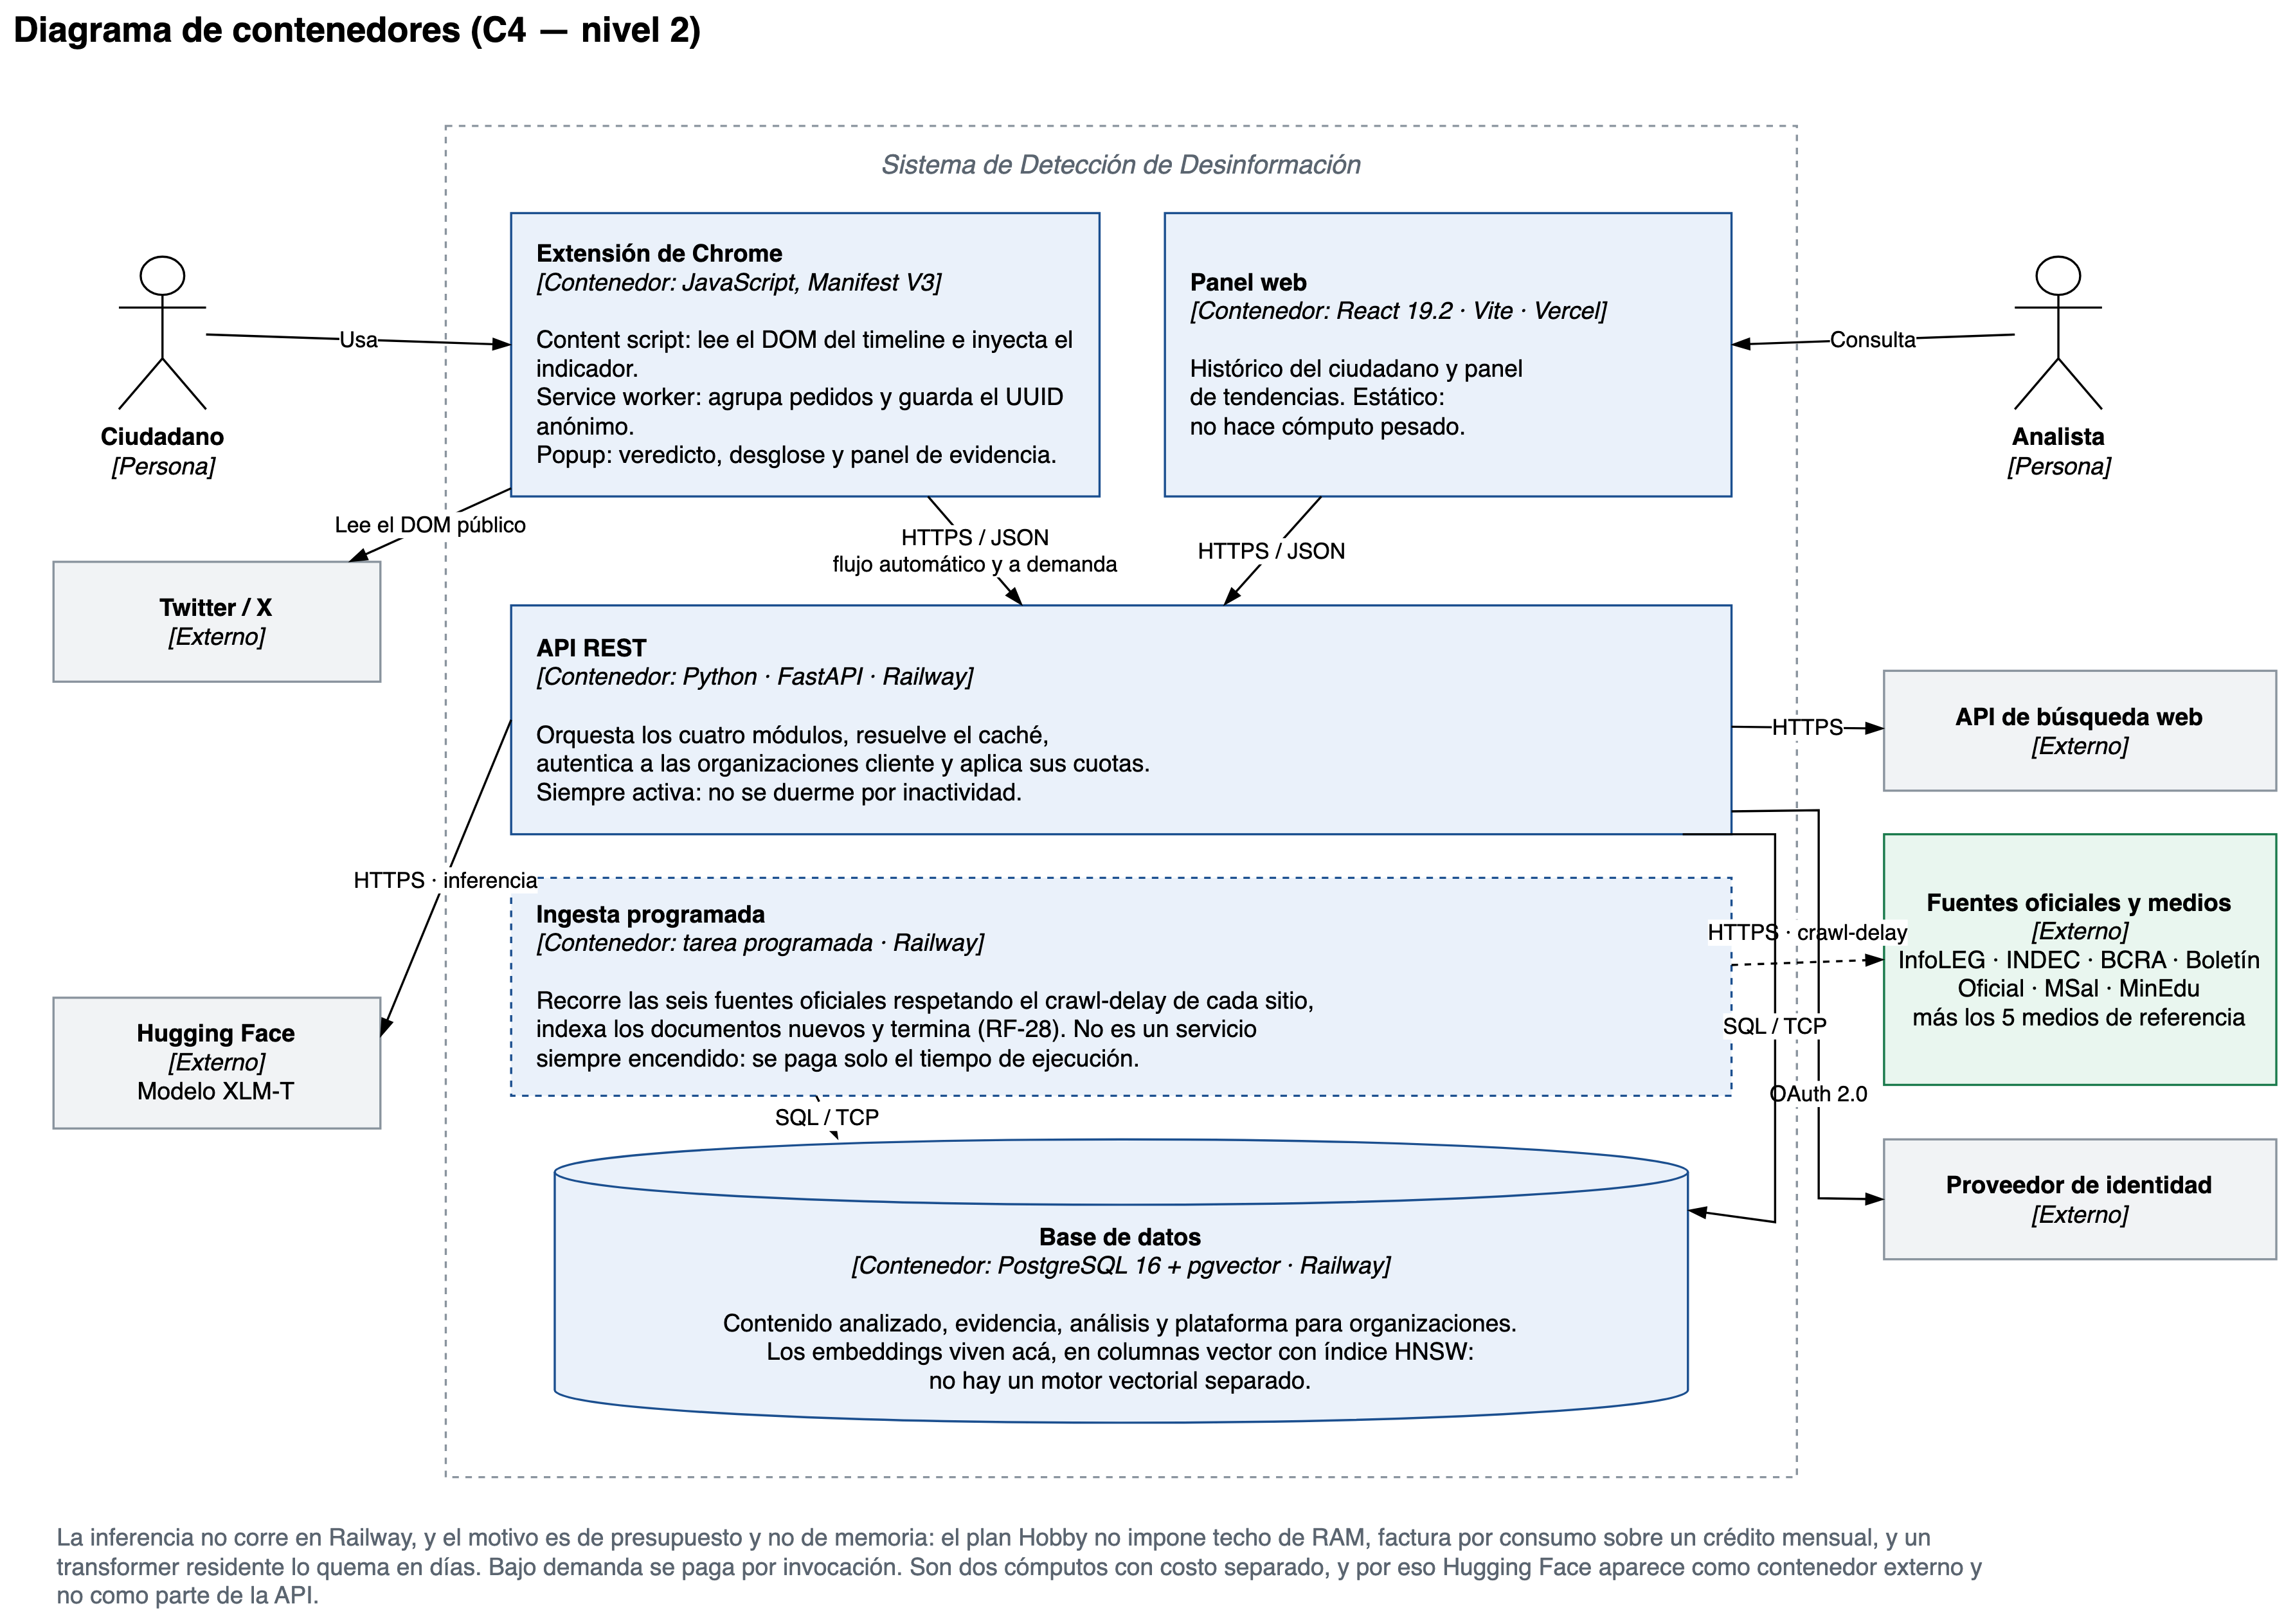
\includegraphics[width=0.95\linewidth]{chapters/figures/c4-contenedores}
  \caption{Modelo C4, nivel 2: diagrama de contenedores. Fuente: elaboración propia.}
  \label{fig:c4-contenedores}
\end{figure}
\end{landscape}

La extensión se organiza en un componente que se ejecuta en el hilo de la página, encargado de leer el documento e insertar el indicador, y un componente de segundo plano que agrupa los pedidos, custodia el identificador anónimo y establece la comunicación con el servicio. La separación no es un detalle de implementación: el primero comparte el hilo de ejecución con la página visitada, razón por la cual RNF-04 le impone un techo de 50 milisegundos por publicación, y todo trabajo que exceda la lectura del documento y la inserción del indicador debe ocurrir en el segundo.

El panel web se sirve como aplicación estática, decisión posible porque no ejecuta cómputo alguno. La API permanece siempre activa: los planes gratuitos que suspenden el servicio ante la inactividad son incompatibles con una extensión que consulta en tiempo real durante el recorrido de la línea de tiempo. Las tecnologías concretas de cada contenedor, con sus versiones, se detallan en la Sección~\ref{sec:tecnologias}.

\subsubsection{Vista de componentes}

El tercer nivel, que presenta la Figura~\ref{fig:c4-componentes}, describe la organización interna de la API.

\begin{landscape}
\begin{figure}[t]
  \centering
  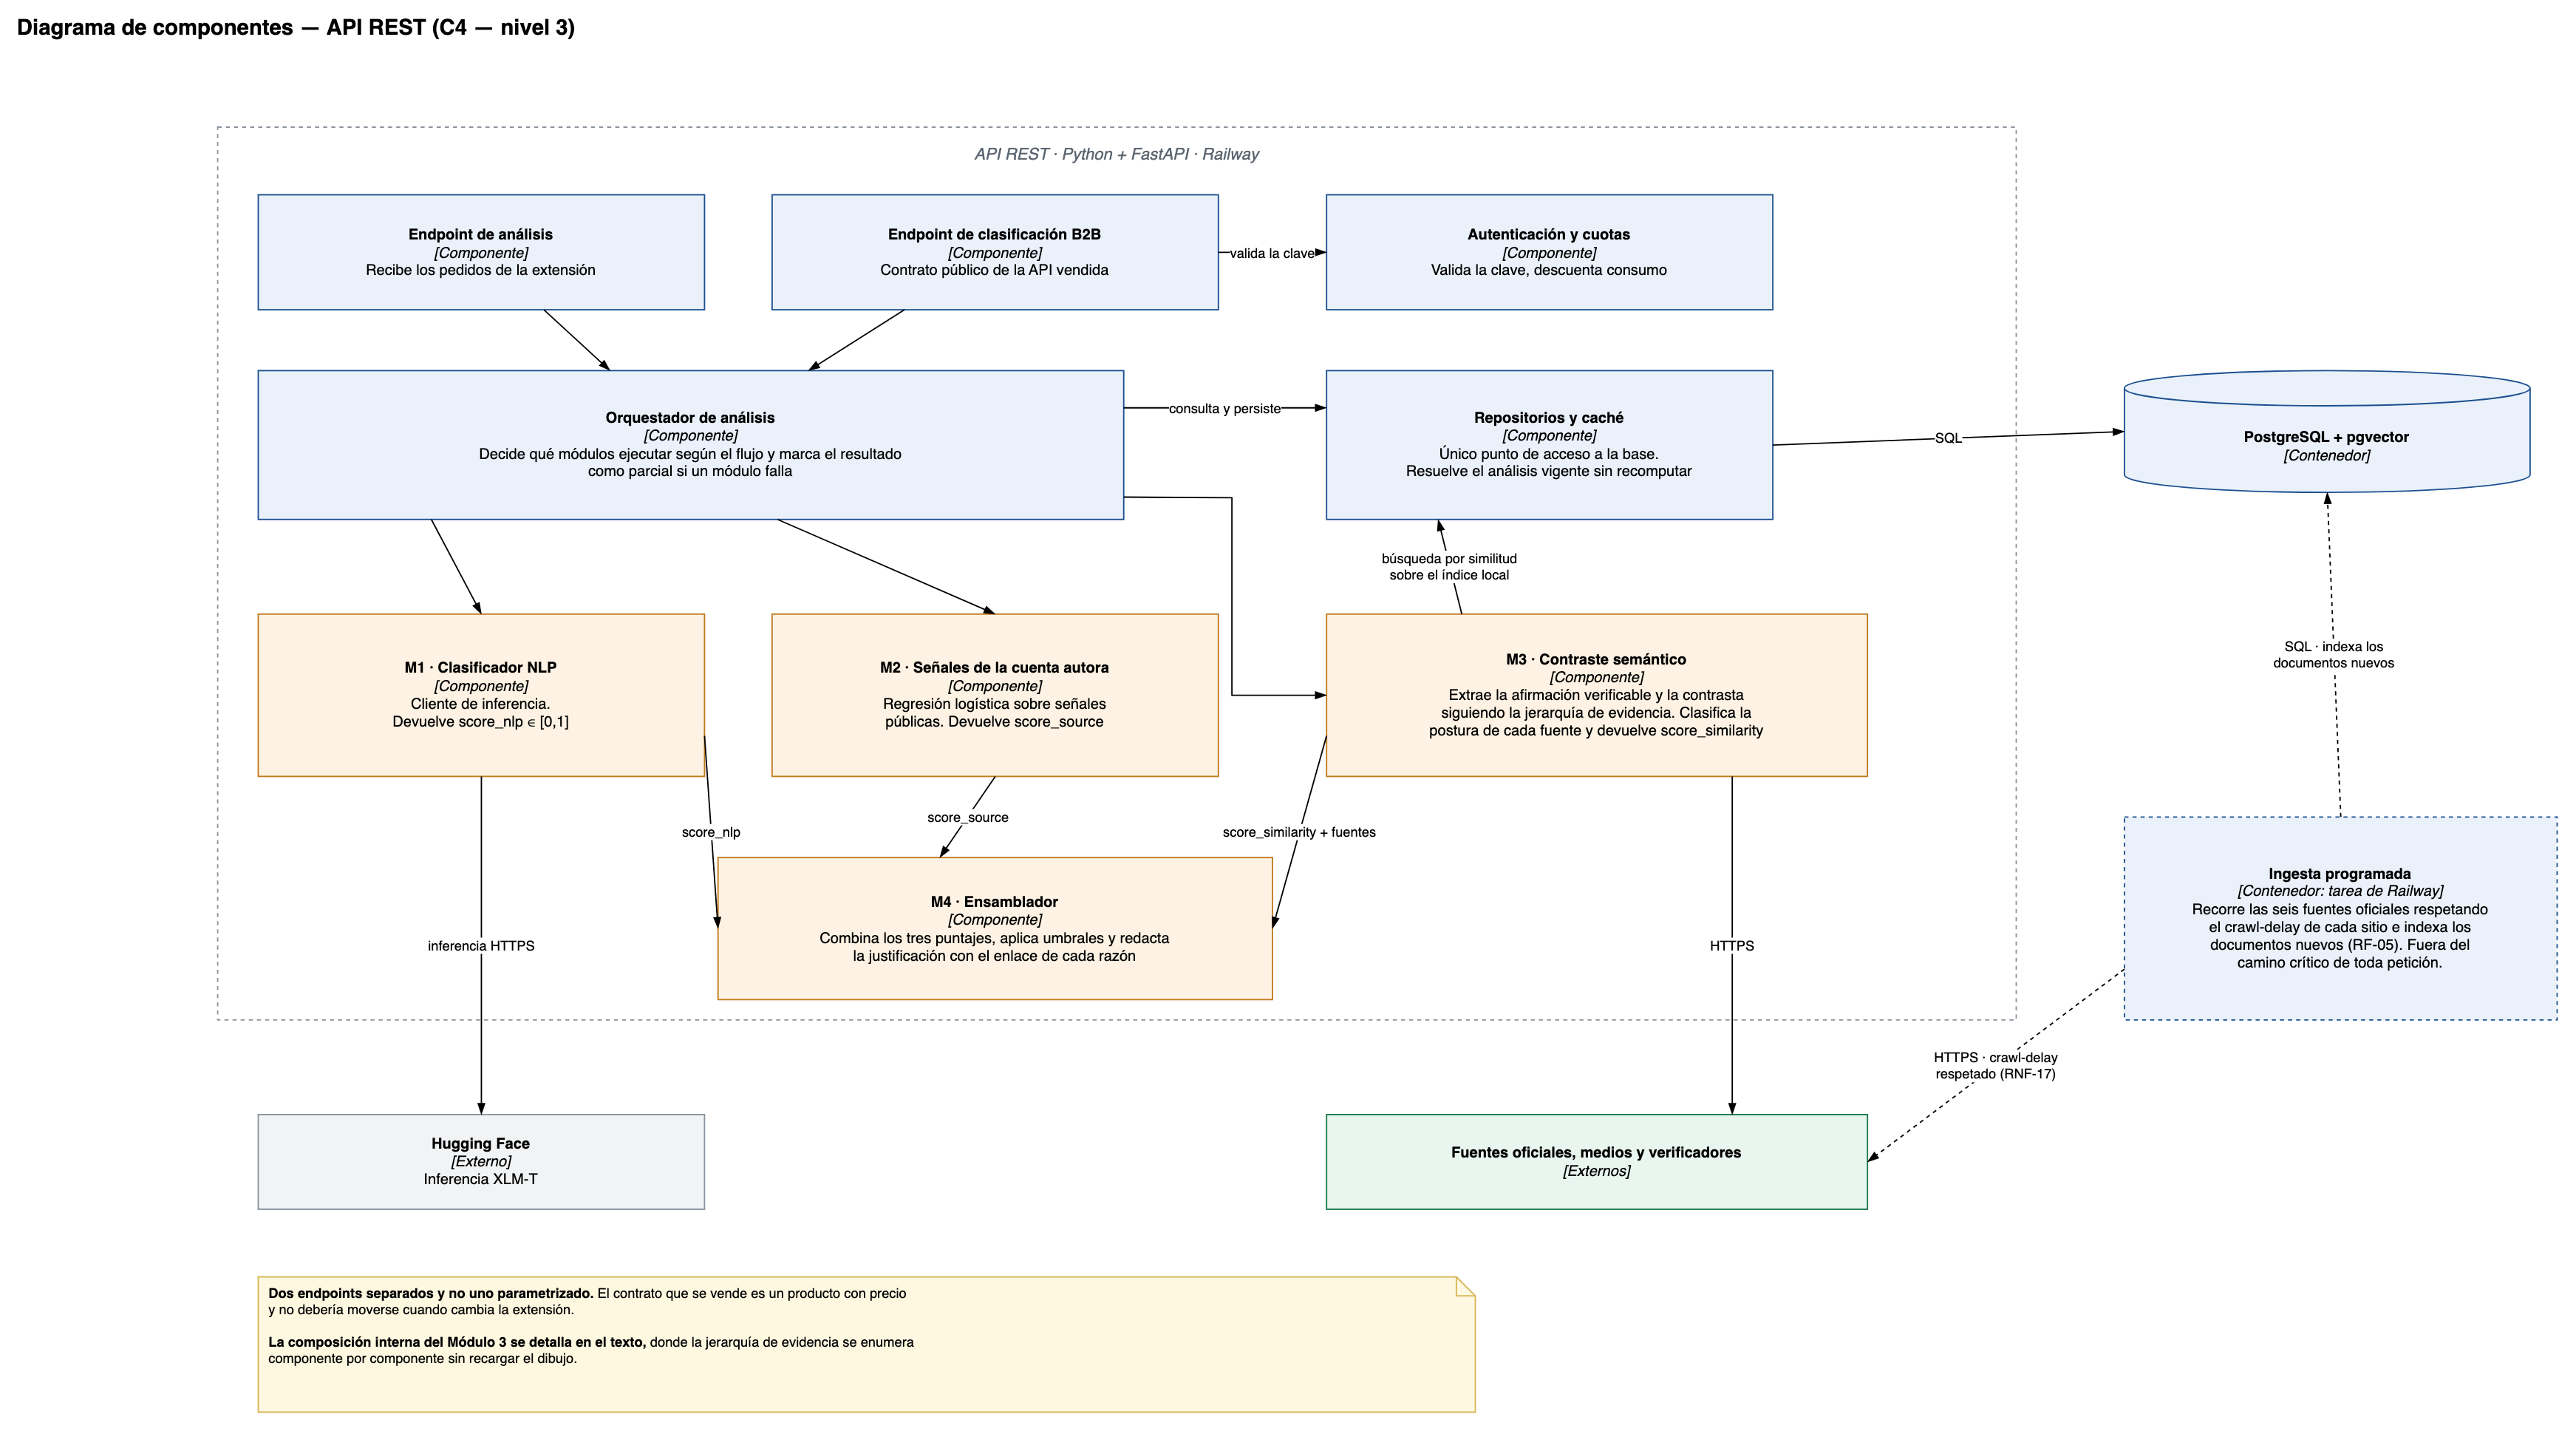
\includegraphics[width=0.95\linewidth]{chapters/figures/c4-componentes}
  \caption{Modelo C4, nivel 3: diagrama de componentes de la API. Fuente: elaboración propia.}
  \label{fig:c4-componentes}
\end{figure}
\end{landscape}

El sistema expone dos puntos de entrada diferenciados y un componente de autenticación y cuotas que protege al segundo. Que se trate de dos interfaces separadas y no de una sola parametrizada responde a una decisión deliberada: el contrato que se comercializa es un producto con precio propio y no debería modificarse cuando cambia la extensión.

El orquestador concentra la decisión de los dos flujos. Recibe el pedido, consulta el análisis vigente y, según el origen de la solicitud, ejecuta únicamente el primer módulo o los cuatro. Es además el componente que marca el resultado como parcial cuando un módulo falla, en lugar de permitir que el ensamblador promedie sobre datos ausentes.

La ponderación con que el ensamblador combina las tres señales no es uniforme. El segundo módulo interviene con un peso deliberadamente menor que el clasificador y que el contraste con evidencia externa, decisión que responde al hallazgo expuesto en la Sección~\ref{sec:entrevistas}: las señales de la cuenta autora poseen valor informativo alto, dado que son la primera operación del proceso de verificación tanto en el usuario profesional como en el segmento primario, pero validez probatoria baja, puesto que el distintivo de verificación y el volumen de seguidores se compran y, por lo tanto, manipulables. El módulo se conserva porque el usuario consulta esa información de todos modos, y se exhibe en el desglose por módulo, pero el veredicto se apoya en las dos señales que guardan relación directa con la afirmación analizada. Los pesos son configurables sin nuevo despliegue según establece RNF-16.

El tercer módulo aparece en el diagrama como un componente único; su composición interna se detalla aquí para preservar la legibilidad de la figura sin sacrificar el detalle. Esa composición reproduce la jerarquía de evidencia en forma de estructura:

\begin{itemize}
  \item \textbf{Extractor de afirmaciones}, que delega en un LLM la extracción de la afirmación verificable y su clasificación por tipo, y cuyo resultado determina el enrutamiento de la consulta.
  \item \textbf{Enrutador de fuentes oficiales}, de prioridad 1, que según el tipo de afirmación busca por similitud sobre los documentos ya indexados. Consulta el índice local y no el sitio de origen.
  \item \textbf{Cliente de medios de referencia}, de prioridad 2, que consulta los medios socios de ADEPA y mide el consenso entre ellos.
  \item \textbf{Buscador vectorial}, de prioridad 3, que localiza verificaciones previas por similitud. Resulta opcional: cuando no existe verificación equivalente, situación frecuente, el contraste no se degrada.
  \item \textbf{Evaluador de postura}, que clasifica cada fuente como corroborante, contradictoria o neutral y sintetiza el puntaje de contraste junto con el conjunto de fuentes vinculadas.
\end{itemize}

El LLM interviene en tres tareas acotadas: la extracción de la afirmación y de su tipo (RF-04), la recuperación de evidencia (RF-05) y la redacción de la justificación en lenguaje natural (RF-06). Ninguna de ellas produce el puntaje del primer módulo, que proviene del clasificador propio, entrenado para esta tarea según se describe en la Sección~\ref{sec:datos} y servido en un Hugging Face Space sin aceleración gráfica. La división responde a lo que cada componente resuelve mejor: la literatura relevada en la Sección~\ref{ch:antecedentes} señala que los LLM aportan mayor valor en la síntesis de evidencia y en la producción de explicaciones que en la clasificación \parencite{SrbaEtAl2025}, y un clasificador propio vuelve medible el desempeño del primer módulo contra RNF-05. El clasificador recibe el texto de la publicación con el mismo preprocesamiento aplicado durante el entrenamiento, y no la afirmación reformulada por el LLM, de modo que su puntaje no depende de la salida de este último.

La apertura del escalón de medios a más de un centenar de dominios exige una regla de agregación explícita. Si la postura de cada fuente se sumara de forma individual, varias notas que reproducen un mismo cable de agencia superarían por cantidad a un documento oficial, y la jerarquía quedaría determinada por el volumen de resultados de la búsqueda. Por esa razón el evaluador promedia la postura dentro de cada escalón y recién después pondera los escalones entre sí, con pesos de 1,0 para las fuentes oficiales, 0,6 para los medios de referencia y 0,4 para las verificaciones previas, normalizados sobre los escalones que efectivamente aportaron fuentes. Una fuente oficial pesa, en consecuencia, más que el conjunto de los medios, y el consenso periodístico conserva su valor como señal sin sustituir a la evidencia documental. Estos pesos forman parte de la configuración versionada del ensamblado y son, por lo tanto, ajustables sin nuevo despliegue según establece RNF-16.

Los repositorios son el único punto de acceso a la base de datos. La concentración no responde a un criterio de purismo: el buscador vectorial y la caché consultan la misma base que persiste los análisis, y unificar el acceso evita que la elección de la extensión vectorial se propague hacia los módulos.

\subsubsection{Ingesta de fuentes oficiales}

Una versión anterior del diseño consultaba el sitio oficial durante la petición del usuario. Esa consulta en línea resultaba incompatible con RNF-02: el dominio que aloja los contenidos de los ministerios declara una demora de rastreo de diez segundos, mientras que el flujo a demanda dispone de ocho segundos en el percentil 95. Una petición cada diez segundos no ingresa en ese presupuesto, y la alternativa de ignorar la demora declarada contradice de plano la postura desarrollada en la Sección~\ref{sec:legal}, que se apoya en respetar lo que cada sitio declara.

Por esa razón las seis fuentes oficiales se indexan de forma anticipada. Una tarea programada recorre el catálogo de fuentes respetando la demora declarada por cada sitio, extrae el texto de los documentos nuevos, obtiene su representación vectorial, los incorpora al almacén de documentos y actualiza la fecha de la última corrida. Concluida esa tarea, el proceso finaliza: no se trata de un servicio permanentemente activo, con lo que solo se factura su tiempo de ejecución.

Las consecuencias de la decisión son mejoras y no concesiones. RNF-02 se cumple con margen, dado que la consulta del enrutador pasa a resolverse de forma local sobre el mismo índice que ya empleaba el buscador vectorial. La demora de rastreo se respeta de forma efectiva, puesto que la espera queda fuera del camino crítico de toda petición de usuario. Y la postura legal se refuerza, al sustituir una consulta sincrónica por cada publicación observada por un acceso espaciado y de baja frecuencia.

\subsubsection{Alcance implementado en el prototipo}
\label{sec:alcance-implementado}

El diseño descrito en esta sección corresponde al sistema completo. El prototipo construido para la validación implementa un subconjunto, y las diferencias se declaran porque condicionan la lectura de los resultados de la Sección~\ref{sec:evaluacion-clasificador}. El tercer módulo no cuenta con el índice local de fuentes oficiales ni con la ingesta programada: la recuperación de evidencia se resuelve con la herramienta de búsqueda web del proveedor del LLM, restringida a los dominios de la jerarquía de evidencia, y su resultado atraviesa el filtro propio de dominios antes de llegar al combinador. El mismo LLM clasifica la postura de cada fuente. La búsqueda vectorial de verificaciones previas queda subsumida en esa búsqueda, que incluye a los verificadores entre los dominios admitidos.

La decisión prioriza un módulo de contraste en funcionamiento sobre la arquitectura que mejor respeta las restricciones del sistema en producción. La búsqueda web resuelve la jerarquía completa con una sola llamada y sin infraestructura propia, a costa de depender de un tercero para la recuperación y de no garantizar la demora de rastreo que motivó la ingesta anticipada, cuyo cumplimiento queda delegado en el proveedor de la búsqueda. Por el mismo motivo, el prototipo persiste los análisis en SQLite y no en PostgreSQL con \texttt{pgvector}, que solo resultaba necesario para el índice de \textit{embeddings}. El índice local, la ingesta programada y la migración del motor de base de datos constituyen la primera línea de trabajo futuro sobre el tercer módulo. El segundo módulo se encuentra recortado de manera deliberada: devuelve un valor identificado como no implementado y pesa cero en el combinador, de modo que ningún valor no medido participa del puntaje final.

\subsubsection{Recorrido de la información}

La Figura~\ref{fig:flujo-informacion} presenta el recorrido completo mediante un diagrama de actividad organizado en cinco calles. Su elemento central es la bifurcación que separa los dos flujos.

\begin{landscape}
\begin{figure}[t]
  \centering
  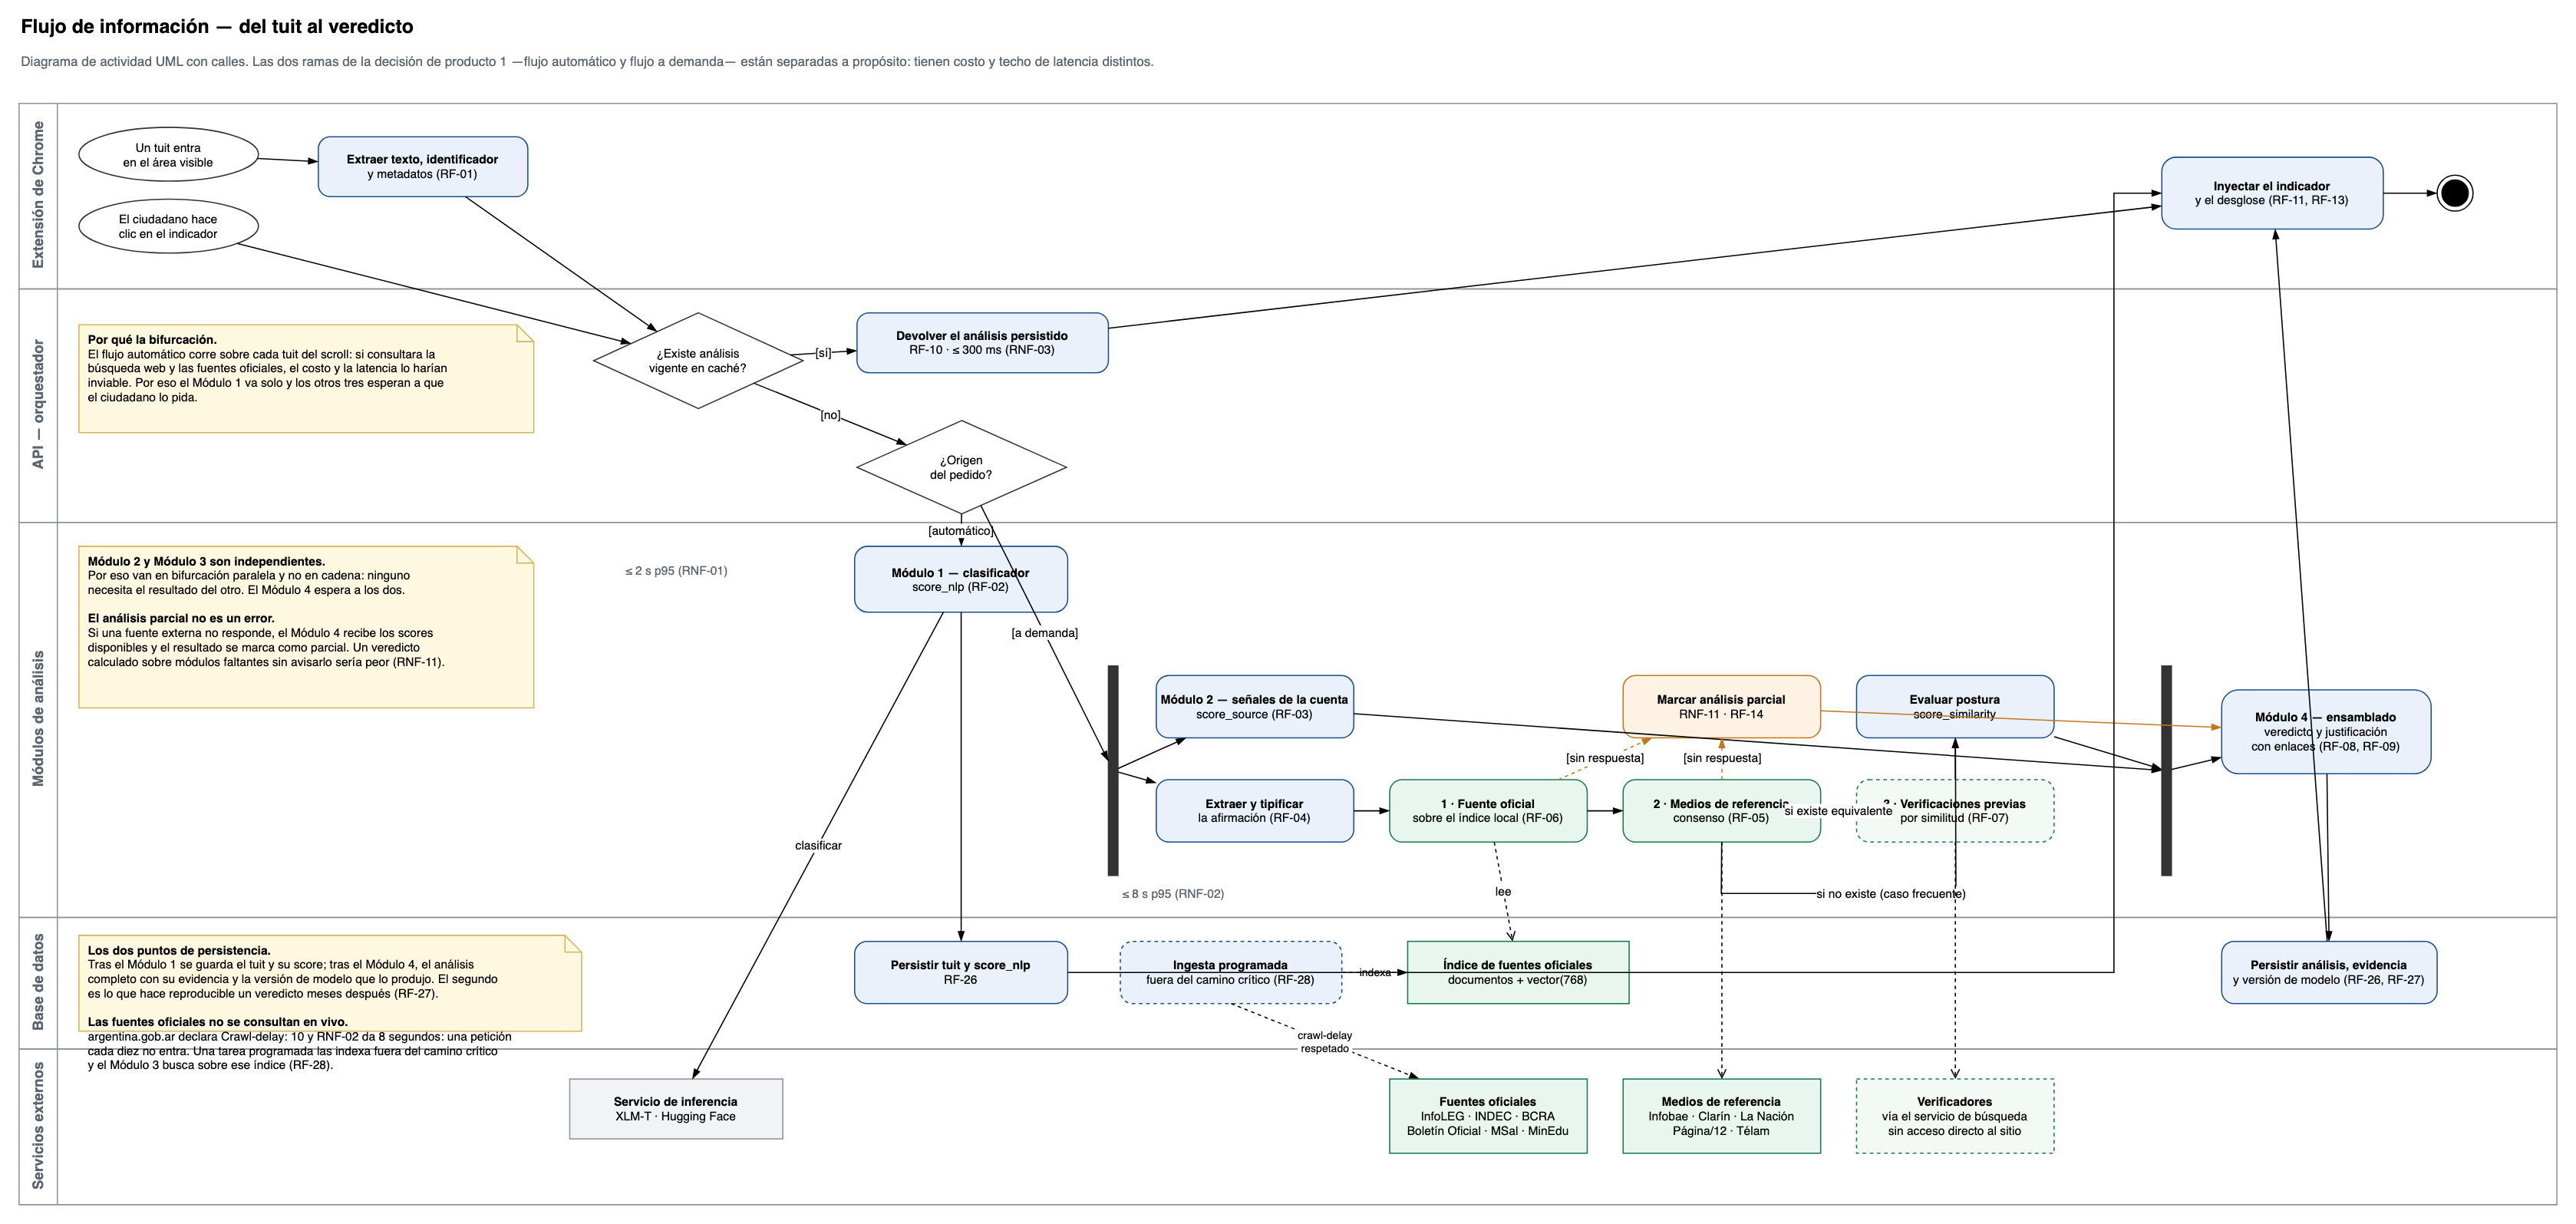
\includegraphics[width=0.95\linewidth]{chapters/figures/flujo-informacion}
  \caption{Diagrama de flujo de información, con las dos entradas, la bifurcación entre el flujo automático y el flujo a demanda, y el camino de excepción hacia el análisis parcial. Fuente: elaboración propia.}
  \label{fig:flujo-informacion}
\end{figure}
\end{landscape}

El recorrido presenta dos entradas y una única salida. La entrada automática corresponde a una publicación que ingresa en el área visible; la entrada a demanda, a la selección de un indicador ya presentado. Ambas convergen en la misma pregunta, si existe un análisis vigente, y solo después se separan según el origen del pedido. La rama automática ejecuta únicamente el primer módulo y dispone de dos segundos; la rama a demanda ejecuta los tres restantes y dispone de ocho.

Dentro de la rama a demanda, el segundo y el tercer módulo se ejecutan en paralelo, representados mediante una bifurcación y una unión. La disposición no es una licencia del dibujo: ambos módulos son independientes, puesto que uno evalúa la cuenta y el otro la afirmación sin que ninguno requiera el resultado del otro, y el cuarto módulo espera a ambos. Representarlos en cadena sugeriría una dependencia inexistente y transmitiría la impresión de que sus latencias se suman cuando en realidad se solapan.

Dentro del tercer módulo, el orden de las tres consultas responde a la jerarquía de evidencia. Del nodo de medios parten dos aristas hacia la evaluación de postura: una atraviesa la consulta de verificaciones previas y la otra la omite. Esta segunda es el camino frecuente, y su representación explícita deja constancia de que la ausencia de una verificación previa no degrada el resultado.

El diagrama presenta dos puntos de persistencia y no uno. Tras el primer módulo se registran la publicación y su puntaje de texto; tras el cuarto, el análisis completo con su evidencia y la versión de modelo que lo produjo. El segundo es lo que vuelve reproducible un veredicto meses después, exigencia del trabajo experimental previsto. El camino de excepción desemboca en un nodo de análisis parcial que alimenta de todos modos al cuarto módulo: devolver un error desaprovecharía el trabajo ya realizado, y promediar sobre los módulos disponibles sin advertirlo produciría un veredicto de menor calidad sin que nadie lo advirtiera.

\subsubsection{Vistas de secuencia}

El comportamiento dinámico se documenta mediante dos diagramas y no uno, por la misma razón por la cual RNF-01 y RNF-02 comprometen números distintos: se trata de dos recorridos con actores, costos y techos de latencia diferentes, y su superposición en un único diagrama con fragmentos anidados los volvería ilegibles sin aportar información adicional.

\begin{landscape}
\begin{figure}[t]
  \centering
  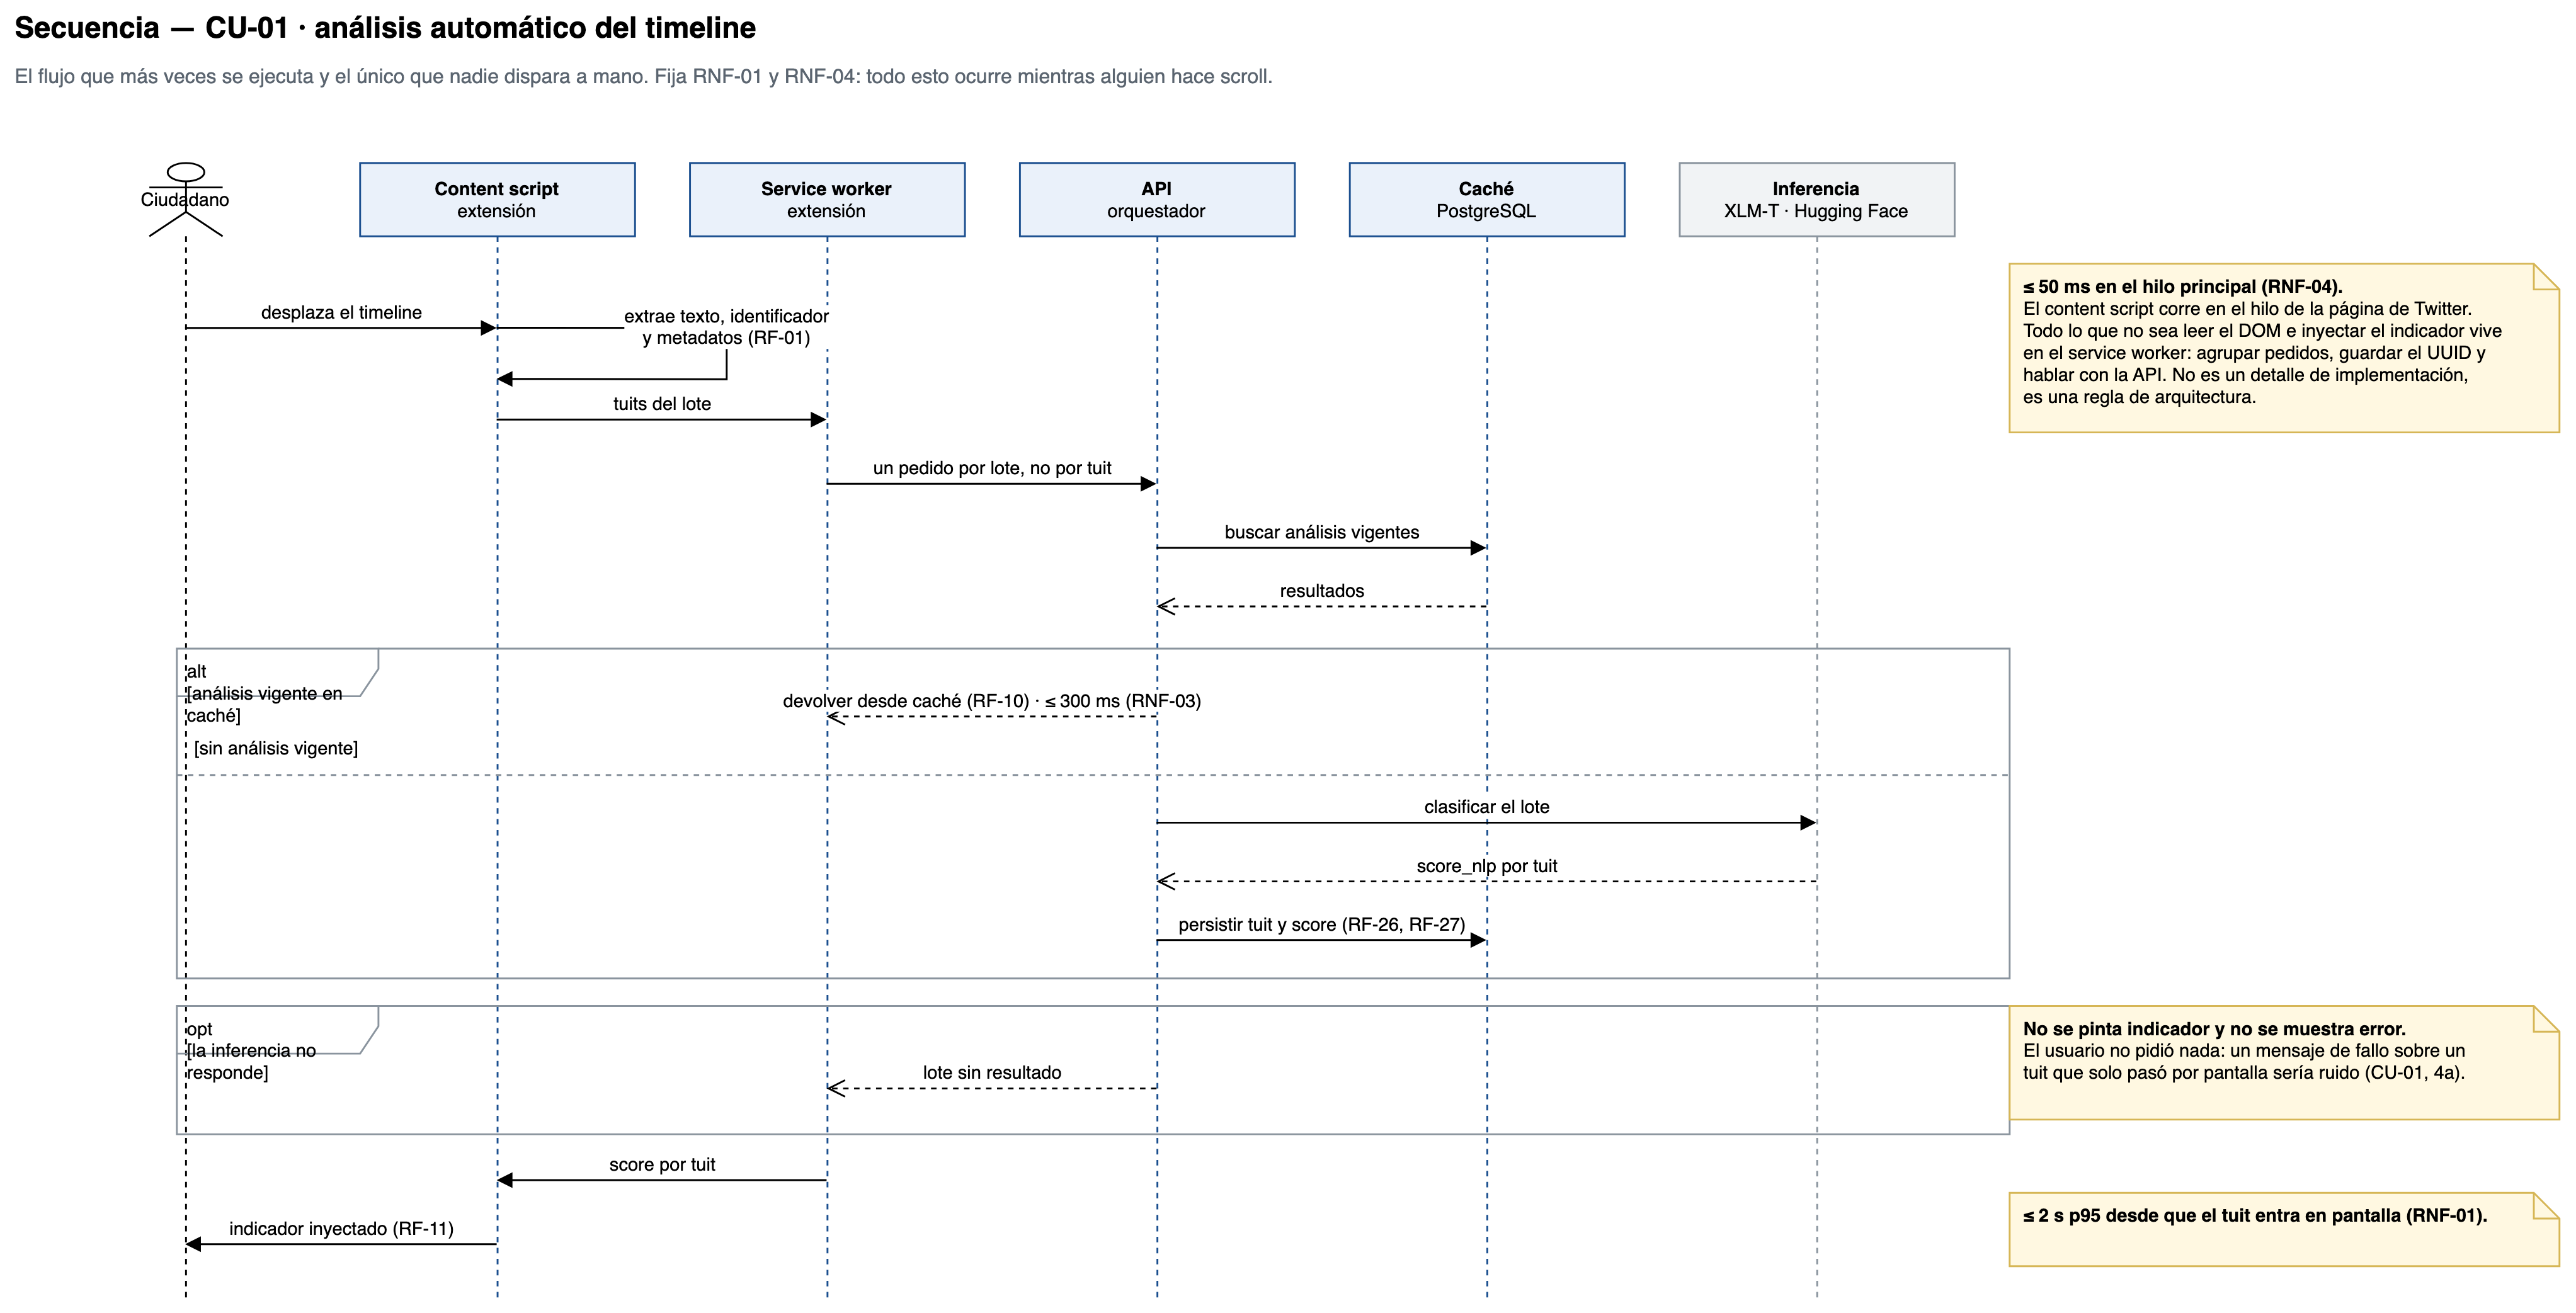
\includegraphics[width=0.95\linewidth]{chapters/figures/secuencia-cu01}
  \caption{Diagrama de secuencia del flujo automático. El fragmento alternativo separa la resolución desde la caché del recorrido completo contra el servicio de inferencia. Fuente: elaboración propia.}
  \label{fig:secuencia-cu01}
\end{figure}
\end{landscape}

La Figura~\ref{fig:secuencia-cu01} corresponde al flujo automático. El mensaje determinante es el que parte del componente de segundo plano hacia la API: se emite uno por lote de publicaciones visibles y no uno por publicación, agrupamiento sin el cual el recorrido de la línea de tiempo generaría una petición por cada elemento que ingresa en pantalla. Un fragmento opcional cubre el fallo del servicio de inferencia, y su resolución es deliberadamente silenciosa: no se presenta indicador y tampoco mensaje de error, dado que el usuario no formuló solicitud alguna y una advertencia sobre una publicación que apenas atravesó la pantalla constituiría ruido.

\begin{landscape}
\begin{figure}[t]
  \centering
  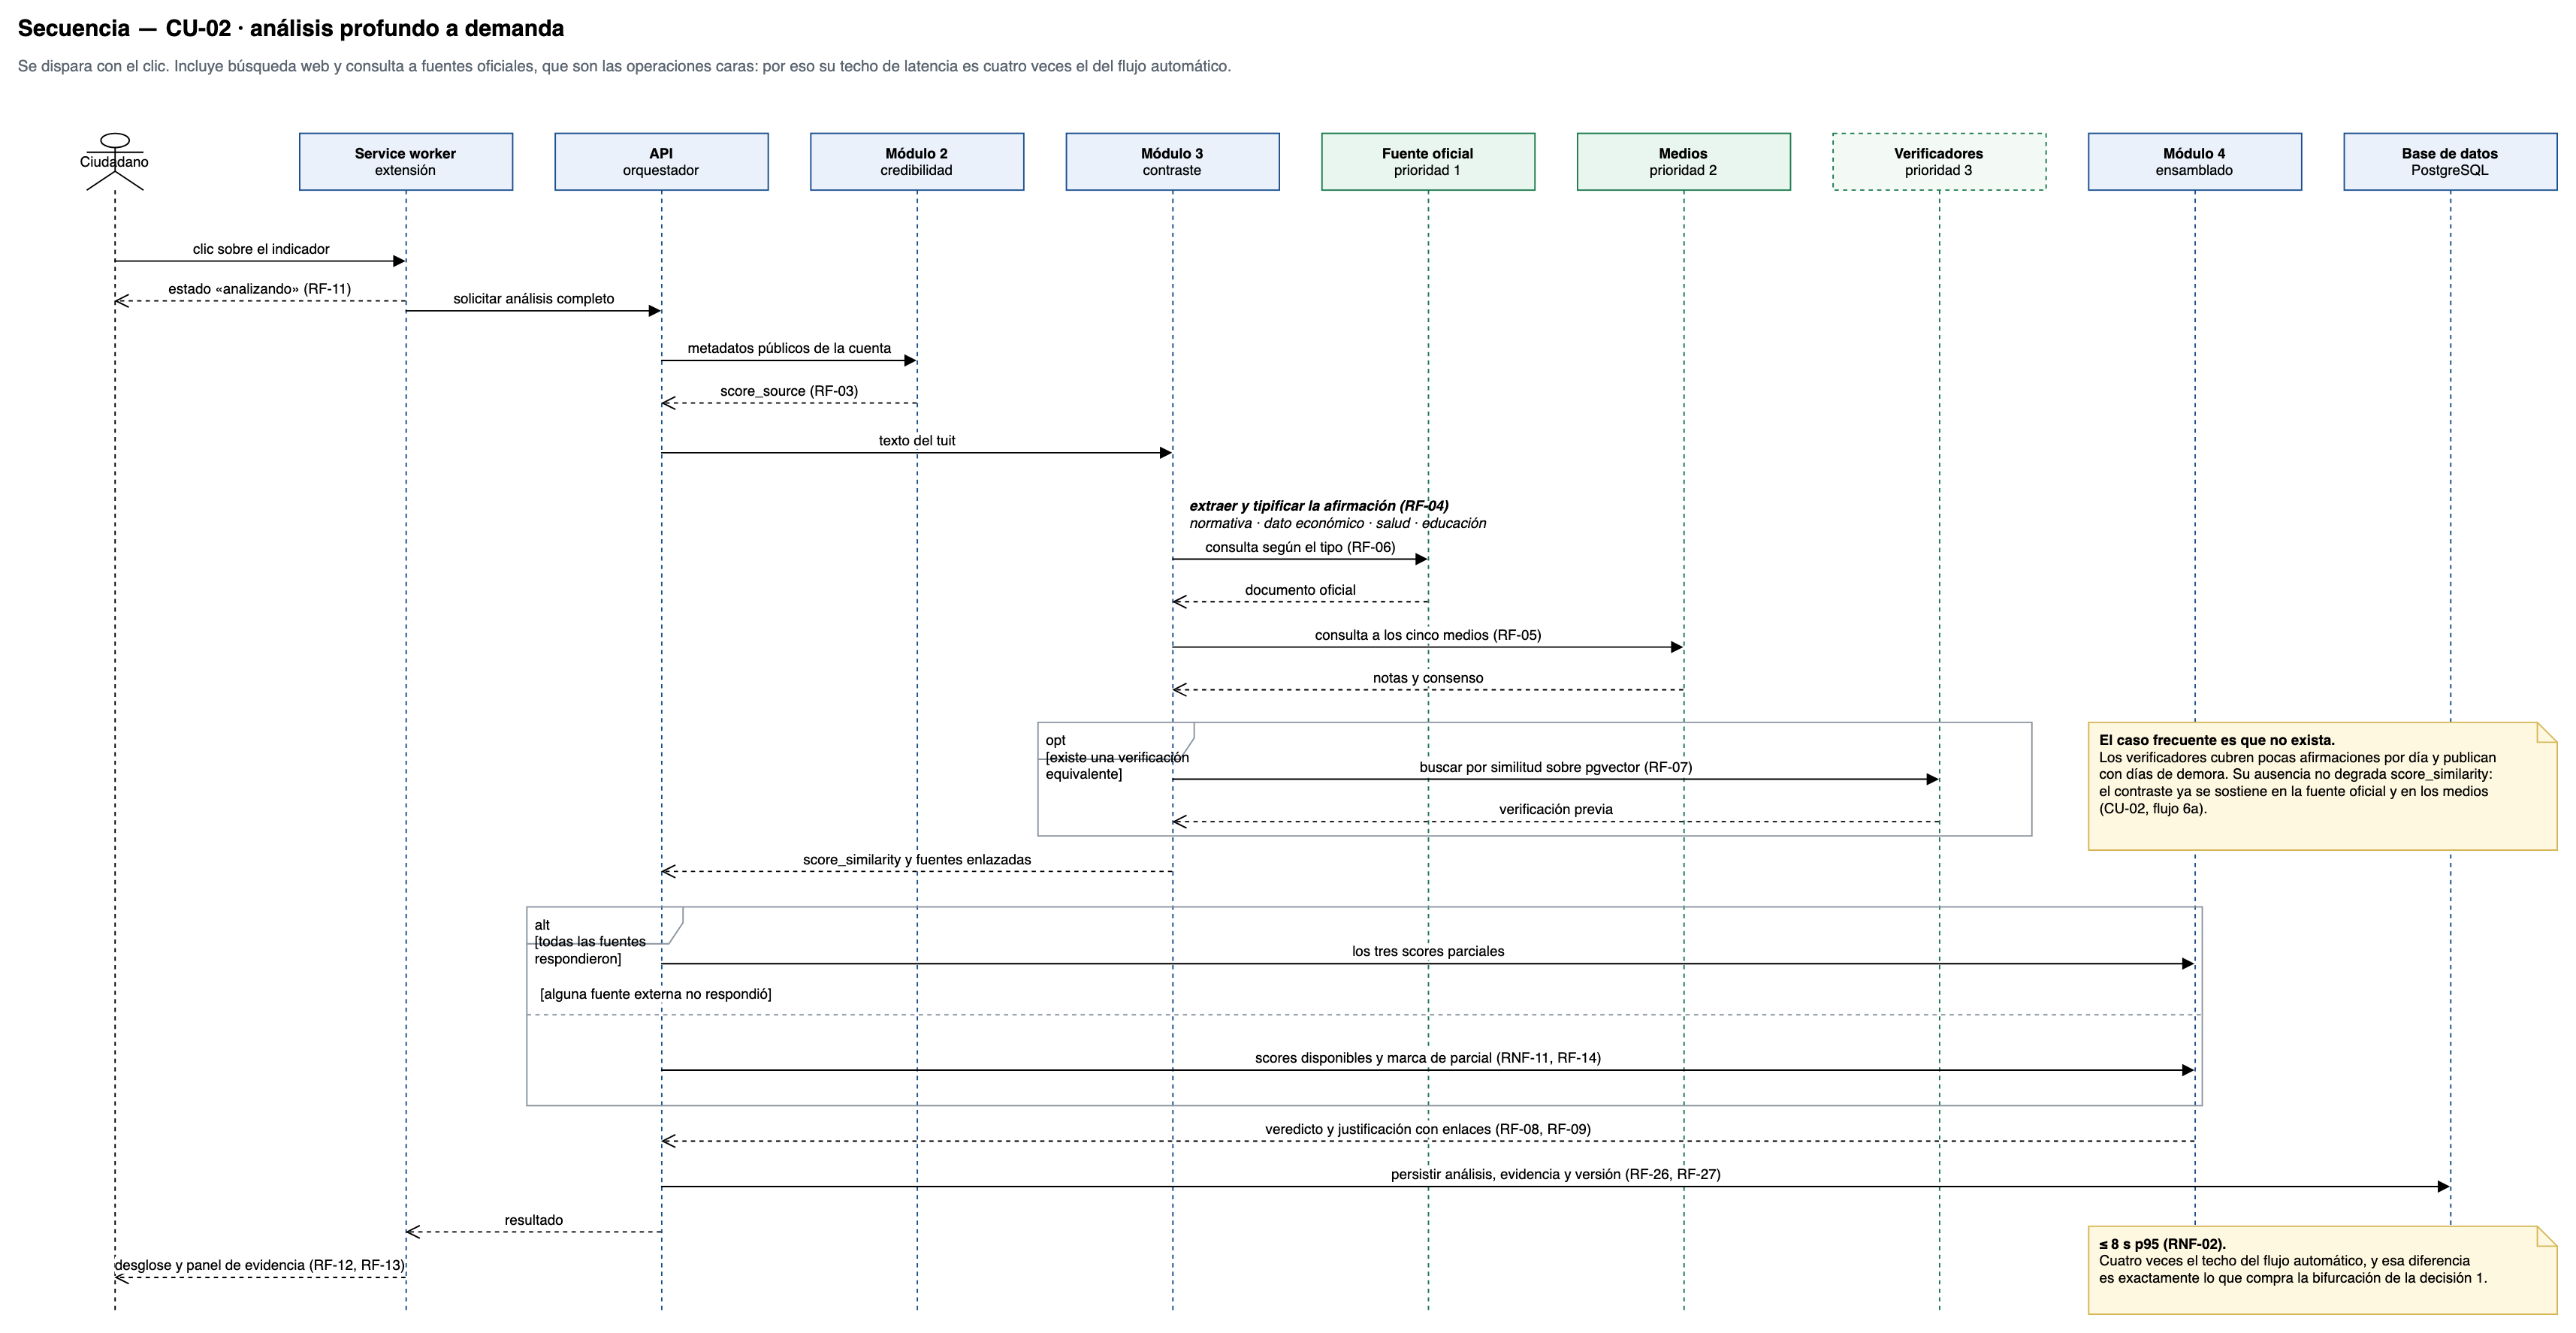
\includegraphics[width=0.95\linewidth]{chapters/figures/secuencia-cu02}
  \caption{Diagrama de secuencia del flujo a demanda, con el tercer módulo desagregado en sus tres fuentes y el fragmento de degradación hacia el análisis parcial. Fuente: elaboración propia.}
  \label{fig:secuencia-cu02}
\end{figure}
\end{landscape}

La Figura~\ref{fig:secuencia-cu02} corresponde al flujo a demanda y desagrega el tercer módulo en sus tres fuentes. La consulta a los verificadores se encuentra dentro de un fragmento opcional, y el retorno del módulo se produce igualmente cuando ese fragmento no se ejecuta. El fragmento alternativo del cierre corresponde a la degradación: si alguna fuente externa no respondió, el cuarto módulo recibe los puntajes disponibles junto con la marca de análisis parcial, y esa marca alcanza a la pantalla del usuario.

\subsubsection{Decisiones de arquitectura}

La Tabla~\ref{tab:decisiones-arq} reúne las decisiones que estructuran la solución, junto con las alternativas evaluadas y el motivo de su descarte.

\begin{small}
\begin{longtable}{@{}p{4cm} p{4.2cm} p{6cm}@{}}
  \caption{Decisiones de arquitectura, alternativas evaluadas y fundamento de la elección. Fuente: elaboración propia.}
  \label{tab:decisiones-arq} \\
  \hline
  \textbf{Decisión} & \textbf{Alternativas evaluadas} & \textbf{Fundamento} \\
  \hline
  \endfirsthead
  \hline
  \textbf{Decisión} & \textbf{Alternativas evaluadas} & \textbf{Fundamento} \\
  \hline
  \endhead
  \hline
  \endfoot
  Análisis en dos flujos, uno automático y económico y otro a demanda y costoso & Ejecución íntegramente automática; ejecución íntegramente a demanda & La primera no se sostiene en costo ni en latencia; la segunda priva a la extensión de su razón de ser, que consiste en advertir sin mediar solicitud \\
  Inferencia en un servicio externo, separada de la API & Cargar el modelo en el mismo contenedor & Un modelo de aproximadamente 125 millones de parámetros residente agota el crédito mensual en pocos días; bajo demanda se factura por invocación. El techo lo impone RNF-14 \\
  Plataforma de despliegue con base de datos incluida y servicio permanentemente activo & Alternativas sin base incluida y con mayor configuración & Los planes que suspenden el servicio ante la inactividad son incompatibles con una extensión que consulta en tiempo real \\
  Extensión vectorial sobre la misma base relacional & Motores vectoriales dedicados & Implementan el mismo algoritmo de indexación. La ventaja de un motor dedicado aparece por encima del millón de vectores y el prototipo manejará decenas de miles, sin costo adicional y con un servicio menos en el despliegue \\
  Panel web estático y separado del servicio & Servir el panel desde la misma API & No requiere cómputo; separarlo elimina su costo y descarga tráfico del contenedor facturado \\
  Identidad en dos niveles: ciudadano anónimo y organización autenticada & Cuenta única para todos; ausencia de cuentas & El ciudadano no requiere cuenta, y su ausencia elimina el tratamiento de datos personales del usuario. La organización la requiere porque existe un plan y una cuota que facturar \\
  Autenticación de organizaciones delegada en un proveedor externo & Gestión propia de usuarios y contraseñas & Evita almacenar y rotar contraseñas, y reduce la superficie de seguridad sin pérdida funcional \\
  Degradación a análisis parcial & Reintentar hasta obtener todos los módulos; devolver error & Reintentar incumple RNF-02; devolver error desaprovecha los módulos que respondieron. La tercera vía consiste en informar qué falta \\
  Fuentes oficiales indexadas de forma anticipada & Consultarlas durante la petición; planificador dentro del propio proceso del servicio & La demora de rastreo declarada excede el presupuesto de latencia. Un planificador interno introduciría esas esperas en el mismo proceso que debe cumplir RNF-01 \\
\end{longtable}
\end{small}

Cuatro decisiones permanecen abiertas y corresponden a la etapa de implementación: el esquema de reintentos y tiempos de espera por servicio externo, la política de expiración de la caché, la periodicidad exacta de la ingesta para cada fuente y el mecanismo de versionado del contrato de la API. La periodicidad, en particular, admite valores distintos por fuente: el Boletín Oficial publica todos los días hábiles mientras que el organismo de estadística lo hace según su calendario de difusión. Ninguna de las cuatro condiciona las decisiones estructurales descritas en esta sección.

La vista de despliegue, que completa la descripción arquitectónica con la distribución física de los componentes y con la arquitectura de red, se presenta en la Sección~\ref{sec:tecnologias} junto con las tecnologías que la sustentan.

\subsection{Modelo de datos}
\label{sec:modelo-datos}

El sistema persiste el contenido analizado, el resultado de cada análisis y la evidencia que lo respalda sobre un motor relacional PostgreSQL en su versión 16, extendido con \texttt{pgvector} para las columnas de representaciones vectoriales densas (\textit{embeddings}). El modelo se presenta a nivel lógico: entidades, atributos, tipos, claves primarias y foráneas, y cardinalidades. La generación del esquema físico y sus índices de afinamiento corresponden a la etapa de implementación.

El diseño se rige por una regla de corte explícita: toda entidad del modelo debe ser trazable hasta un requerimiento funcional del sistema. La matriz que cierra esta sección es lo que vuelve verificable esa regla, y la única entidad que no la satisface de forma directa queda declarada como excepción argumentada en lugar de omitirse.

\subsubsection{Estructura general}

El modelo comprende diecisiete entidades agrupadas en cinco dominios. La Figura~\ref{fig:der} presenta el diagrama entidad-relación completo, con las veinte relaciones y sus cardinalidades; los atributos se detallan en las tablas de esta sección, decisión que responde a un criterio de legibilidad: un diagrama que incorpore los atributos dentro de cada entidad se vuelve ilegible en formato impreso a partir de la docena de entidades.

La entidad \texttt{analisis} ocupa el centro del esquema y participa de nueve de las veinte relaciones que el diagrama representa. Su posición es consecuencia directa de dos exigencias: la trazabilidad, que obliga a asociar cada análisis a la versión de modelo y a la configuración de pesos que lo produjeron, y la doble propiedad que introduce la plataforma orientada a organizaciones, donde un mismo análisis puede pertenecer a una instalación de la extensión o a una organización cliente, pero nunca a ambas.

La Tabla~\ref{tab:entidades} enumera las entidades por dominio, con su propósito y los requerimientos funcionales que sostienen.

\begin{table}[t]
  \centering
  \small
  \caption{Entidades del modelo de datos, agrupadas por dominio, con los requerimientos funcionales a los que se traza cada una. Fuente: elaboración propia.}
  \label{tab:entidades}
  \begin{tabular}{l p{5.6cm} l}
    \hline
    \textbf{Entidad} & \textbf{Propósito} & \textbf{Requerimientos} \\
    \hline
    \multicolumn{3}{l}{\textit{Dominio 1: Contenido analizado}} \\
    \texttt{tuit} & Texto, métricas públicas y fecha de captura & RF-01, RF-07, RF-16 \\
    \texttt{cuenta} & Señales públicas de la cuenta autora & RF-01, RF-03, RF-16 \\
    \texttt{fuente\_oficial} & Catálogo y estado de la ingesta programada & RF-05 \\
    \texttt{medio\_confiable} & Padrón de medios de referencia, tomado de los socios activos de ADEPA & RF-05, RF-09 \\
    \multicolumn{3}{l}{\textit{Dominio 2: Análisis y evidencia}} \\
    \texttt{analisis} & Puntajes parciales, puntaje final y veredicto & RF-02, RF-06, RF-08 \\
    \texttt{razon} & Justificación en lenguaje natural, ordenada & RF-06 \\
    \texttt{claim} & Afirmación verificable extraída del contenido & RF-04, RF-05 \\
    \texttt{documento} & Documento de una fuente, con su vector & RF-05, RF-09 \\
    \texttt{evidencia} & Vínculo entre un análisis y un documento & RF-05, RF-06, RF-09 \\
    \multicolumn{3}{l}{\textit{Dominio 3, Uso ciudadano}} \\
    \texttt{usuario\_extension} & Identificador local de la instalación & RF-10 \\
    \texttt{reporte} & Aviso de veredicto incorrecto & RF-11 \\
    \multicolumn{3}{l}{\textit{Dominio 4, Trazabilidad del modelo}} \\
    \texttt{modelo\_version} & Punto de control del modelo y su desempeño & RF-11, RF-16 \\
    \texttt{configuracion\_ensamblado} & Pesos y umbrales versionados & RF-16 \\
    \multicolumn{3}{l}{\textit{Dominio 5: Plataforma para organizaciones}} \\
    \texttt{organizacion} & Cliente, con su plan y su cuota & RF-13 \\
    \texttt{usuario\_b2b} & Analista autenticado de una organización & RF-13 \\
    \texttt{api\_key} & Clave de acceso, almacenada resumida & RF-13 \\
    \texttt{consumo\_api} & Registro de cada llamada contra la cuota & RF-13 \\
    \hline
  \end{tabular}
\end{table}

\begin{landscape}
\begin{figure}[t]
  \centering
  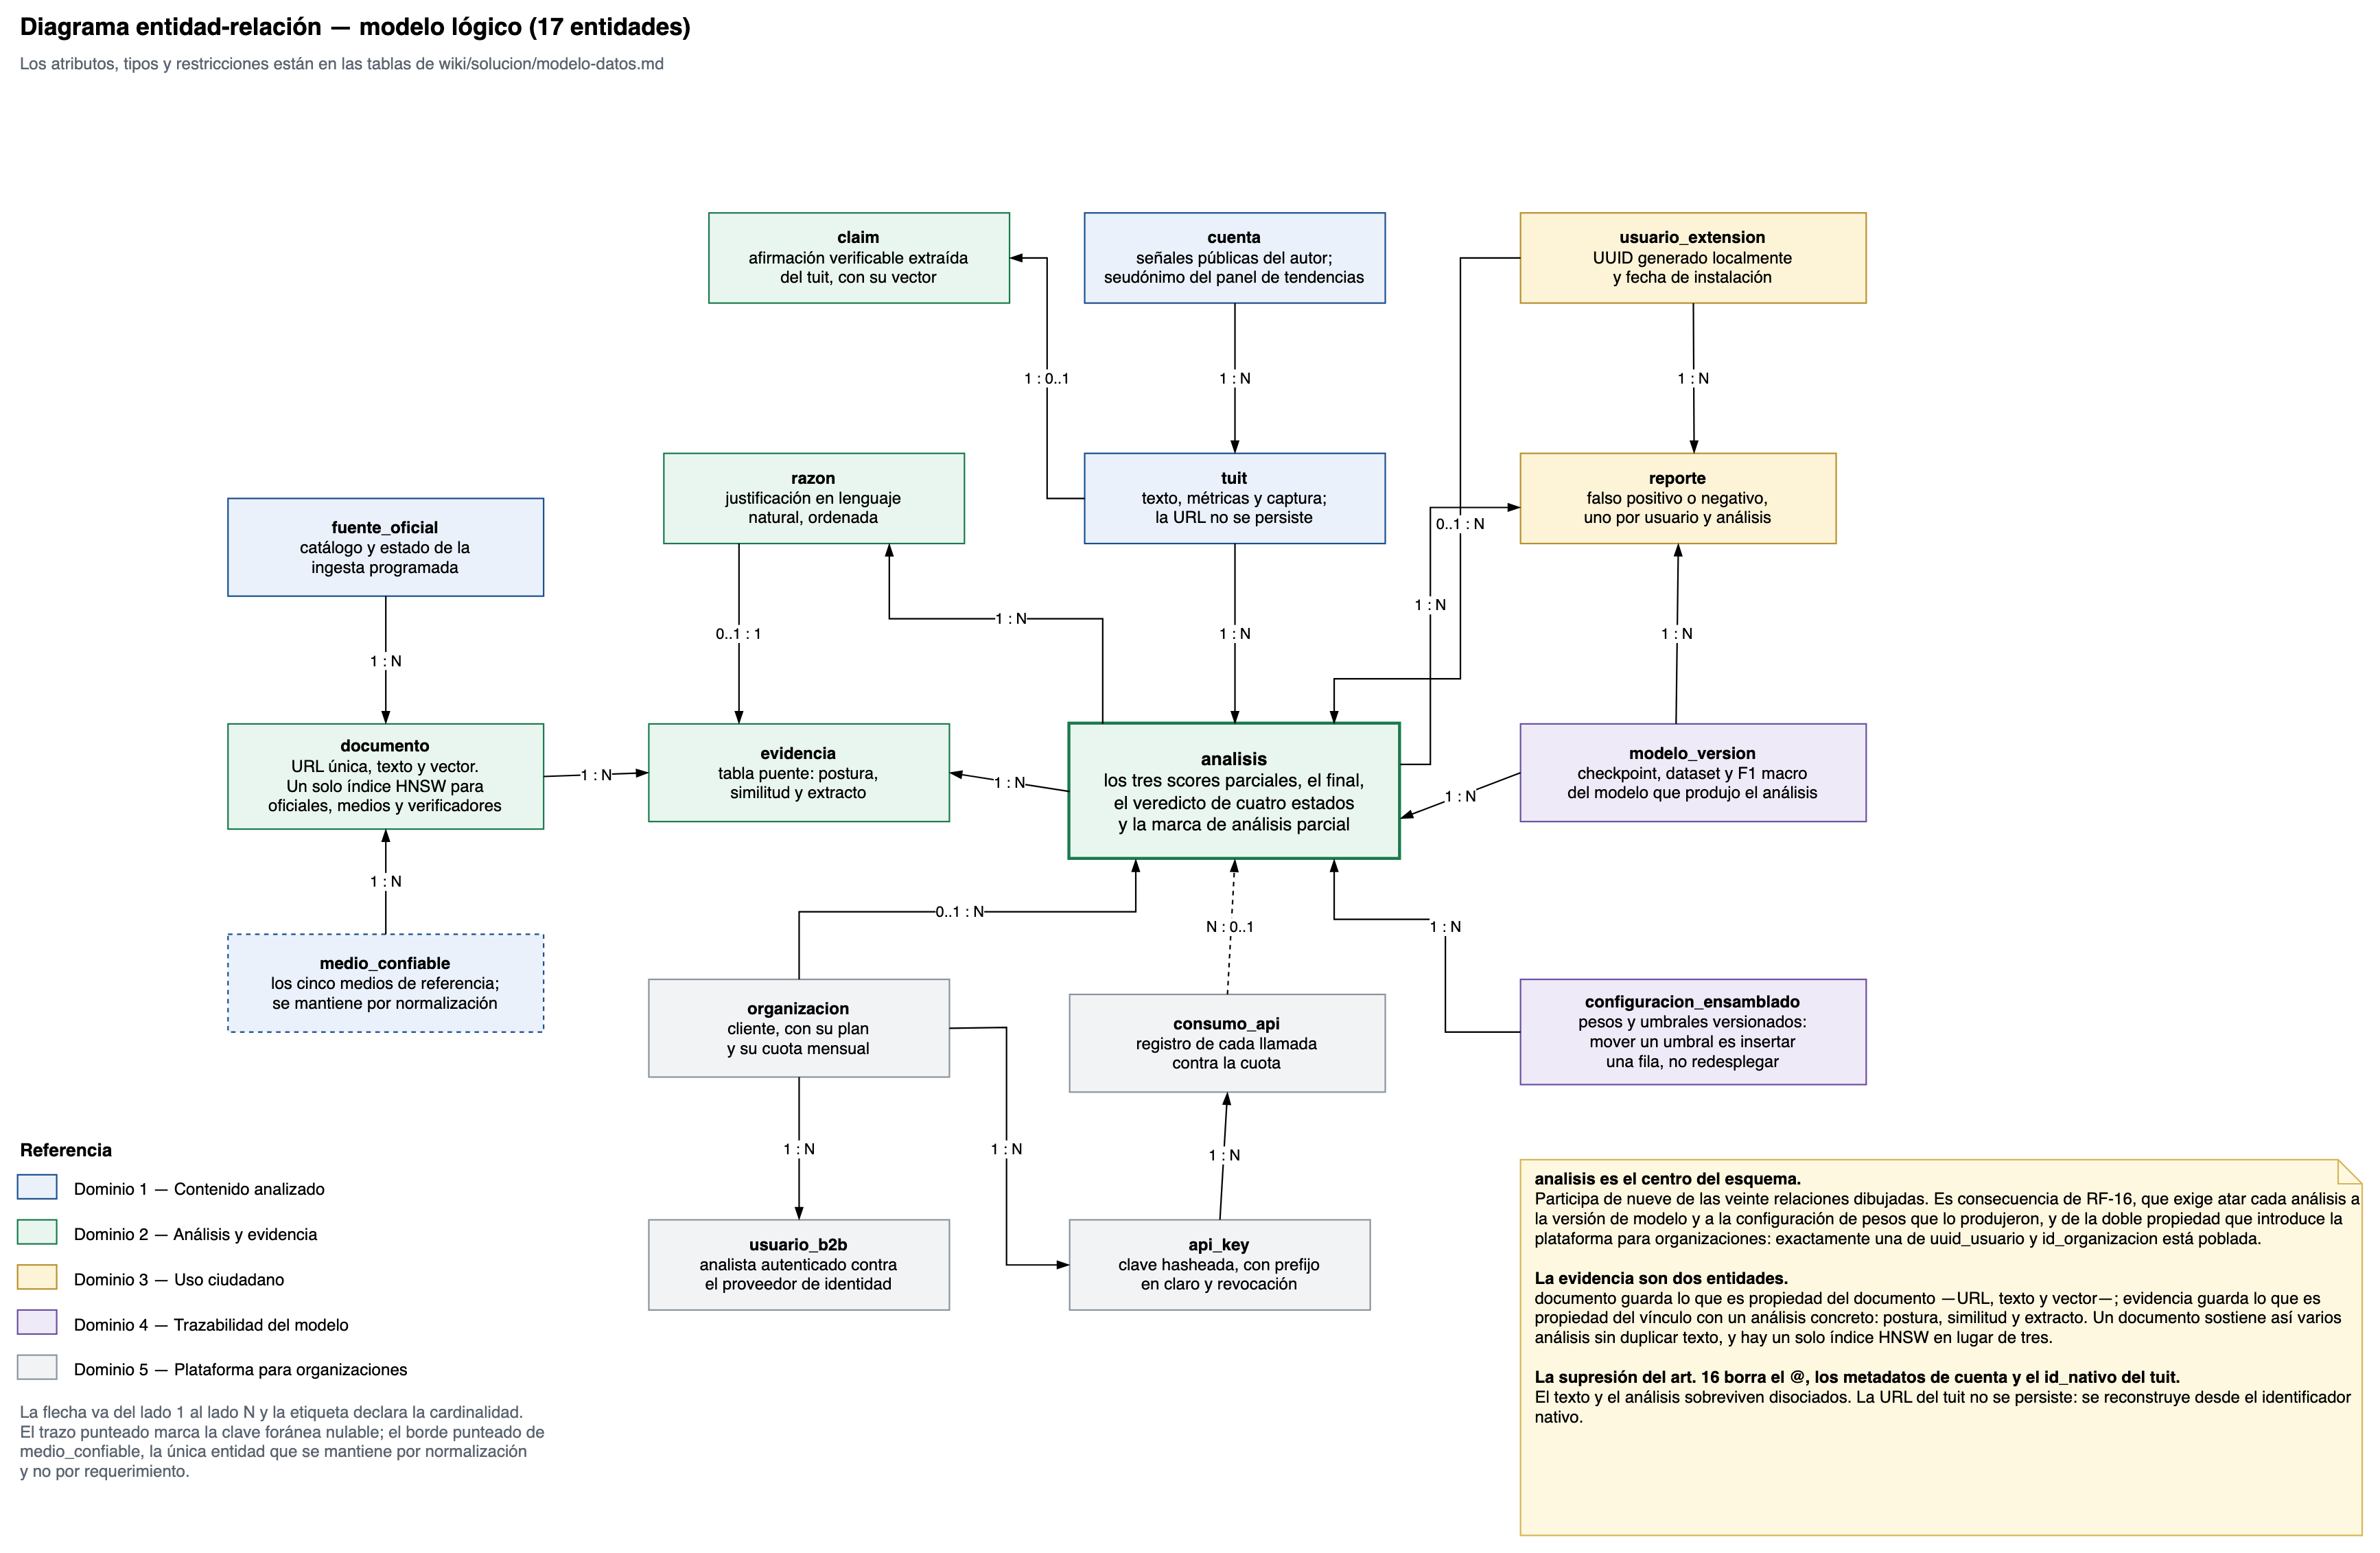
\includegraphics[width=0.95\linewidth]{chapters/figures/der}
  \caption{Diagrama entidad-relación del sistema, a nivel lógico. Las diecisiete entidades se agrupan en cinco dominios, identificados por color. Fuente: elaboración propia.}
  \label{fig:der}
\end{figure}
\end{landscape}

\subsubsection{Decisiones de diseño}

Cinco definiciones del modelo condicionan el resto del sistema y merecen su fundamento, porque el diagrama no las explica por sí solo.

\paragraph{La evidencia se representa mediante dos entidades}

La entidad \texttt{documento} conserva lo que es propiedad del documento recuperado (su dirección única, su texto y su vector) mientras que \texttt{evidencia} funciona como entidad puente y conserva lo que es propiedad del vínculo entre ese documento y un análisis concreto: la postura, la similitud y el fragmento citado. La distinción no es formal: un mismo artículo del Boletín Oficial puede corroborar una afirmación y contradecir otra, con lo cual la postura no es un atributo del documento sino de la relación.

De esa partición se derivan varias consecuencias. En primer lugar, un documento sostiene varios análisis sin que su texto se duplique, cosa que importa cuando una misma norma contradice decenas de publicaciones. En segundo lugar, el esquema mantiene un único índice de búsqueda por vecinos aproximados en lugar de tres: los documentos oficiales, las notas de los medios de referencia y las verificaciones previas conviven en la misma entidad, discriminados por un atributo de tipo de fuente, dado que las tres poblaciones se consultan de idéntica manera. Por último, la presentación jerárquica de las fuentes que exige RF-09 se resuelve mediante un ordenamiento sobre ese atributo, y no mediante la unión de tres relaciones distintas.

\paragraph{Existe una única fila de análisis por publicación y versión de modelo}

El análisis nace durante el flujo automático con el puntaje del clasificador de lenguaje natural y se completa mediante una actualización cuando se ejecuta el flujo a demanda; un atributo de profundidad distingue ambos estados. La alternativa (registrar dos filas, una por flujo) habría obligado a determinar cuál de las dos es el veredicto de la publicación en el histórico personal y en la agregación por tema del panel de tendencias, y esa pregunta no admite una respuesta satisfactoria.

\paragraph{El veredicto admite cuatro valores y la marca de análisis parcial es independiente}

A los tres niveles que define RF-06 se suma un cuarto estado, denominado \textit{sin contraste externo}, que se emite cuando ningún módulo de contraste encontró fuente alguna. Su existencia es lo que vuelve exigible RNF-06: la ausencia de evidencia se comunica como ausencia, con una representación visual propia y sin porcentaje, en lugar de presentarse con la apariencia de un veredicto.

Ese estado y la marca de análisis parcial que introduce RF-08 designan situaciones distintas y por eso se representan mediante atributos separados. El estado de contraste indica que un módulo se ejecutó y no halló fuente; la marca de análisis parcial indica que el módulo no pudo ejecutarse. Ambas circunstancias pueden presentarse de forma simultánea, de modo que unificarlas habría alterado el significado de RF-08.

\paragraph{La disociación se resuelve suprimiendo tres atributos}

El ejercicio del derecho de supresión que reconoce el artículo 16 de la Ley 25.326 elimina el nombre de usuario, los metadatos de la cuenta y el identificador nativo de la publicación \parencite{CongresoNacion2000}. El texto, el análisis y la evidencia sobreviven disociados y, al no permitir la atribución a una persona determinada, quedan fuera del alcance de la ley.

Dos decisiones complementarias cierran los caminos por los que la disociación habría resultado reversible. La dirección de la publicación no se persiste: se reconstruye a partir del identificador nativo, ya que conservarla equivalía a guardar el nombre de usuario en texto plano en un segundo atributo. Y el propio identificador nativo se elimina en la supresión, porque permitía recuperar el nombre de usuario consultando la plataforma. El costo de esta decisión se enuncia de forma explícita: la fila suprimida pierde reproducibilidad experimental. Se trata de un costo acotado a las filas efectivamente suprimidas y proporcionado al derecho que se satisface.

Se evaluó y se descartó la alternativa de aplicar una función de resumen al identificador desde el momento de la captura. Esa opción impedía la reutilización del análisis previo que exige RF-07 y la deduplicación en la caché, ambas apoyadas en el identificador nativo, y volvía irreproducible la totalidad del corpus para resolver una situación que afecta a unas pocas filas.

\paragraph{El seudónimo del panel de tendencias es el identificador interno de la cuenta}

RNF-10 exige que ninguna entrega hacia terceros contenga la identidad de la cuenta autora en claro, y la supresión obliga a eliminar el nombre de usuario. La agrupación por el identificador interno satisface ambas condiciones de forma simultánea: al no derivarse del nombre de usuario, es irreversible por construcción y no por fuerza criptográfica, y sobrevive a la supresión sin comprometerla, lo que preserva la serie histórica de la cuenta en el panel. Se descartó aplicar un código de autenticación de mensaje sobre el nombre de usuario, alternativa que habría introducido un derivado del dato personal y una clave secreta que administrar para obtener un resultado equivalente.

\subsection{Tecnologías utilizadas}
\label{sec:tecnologias}

Las versiones que se detallan a continuación se fijaron y verificaron contra el registro de paquetes o el sitio de cada proyecto durante agosto de 2026. Fijarlas responde a una razón concreta: el desarrollo se extiende a lo largo de un año, y una dependencia que alcanza su fin de vida a mitad de camino es un riesgo de cronograma y no un detalle de instalación.

\subsubsection{Componentes por capa}

La Tabla~\ref{tab:stack} sintetiza las tecnologías adoptadas en cada capa del sistema.

\begin{table}[t]
  \centering
  \small
  \caption{Tecnologías adoptadas por capa, con la versión fijada. Fuente: elaboración propia.}
  \label{tab:stack}
  \begin{tabular}{l l l p{4.5cm}}
    \hline
    \textbf{Capa} & \textbf{Tecnología} & \textbf{Versión} & \textbf{Función} \\
    \hline
    Extensión & TypeScript & 7.0.2 & Lenguaje de la extensión \\
              & Vite & 8.2.1 & Empaquetado multi-entrada \\
    Panel web & React & 19.2.8 & Interfaz del panel \\
              & Recharts & 3.10.1 & Gráficos del panel de tendencias \\
              & Node.js & 24.19.0 & Entorno de construcción \\
    Servicio & Python & 3.14.7 & Lenguaje del servicio \\
             & FastAPI & 0.141.1 & \textit{Framework} de la API \\
             & Uvicorn & 0.52.1 & Servidor de aplicación \\
             & Pydantic & 2.13.4 & Validación de esquemas \\
             & SQLAlchemy & 2.0.51 & Acceso a datos \\
             & psycopg & 3.3.4 & Controlador de PostgreSQL \\
             & httpx & 0.28.1 & Cliente HTTP asíncrono \\
    Ingesta & BeautifulSoup & 4.15.0 & Extracción de texto de documentos \\
    Datos & PostgreSQL & 16.14 & Motor relacional \\
          & \texttt{pgvector} & 0.8.6 & Índice de \textit{embeddings} \\
          & Alembic & 1.19.1 & Migraciones del esquema \\
    Inferencia & Clasificador propio & --- & Primer módulo, servido en un Hugging Face Space \\
               & LLM de terceros & --- & Extracción de la afirmación, recuperación de evidencia y justificación \\
               & \textit{multilingual-e5-base} & 768 dim. & Codificador de \textit{embeddings} \\
    Identidad & OAuth 2.0 / OIDC & --- & Autenticación de organizaciones \\
    \hline
  \end{tabular}
\end{table}

Esta distribución tiene una consecuencia que condiciona el presupuesto de infraestructura. Las bibliotecas asociadas al ajuste fino y a la evaluación de los modelos de lenguaje (\textit{transformers}, \textit{torch} y \textit{sentencepiece}, entre otras) pertenecen al entorno de experimentación y no forman parte de la imagen que se despliega. El contenedor del servicio se comunica con la plataforma de inferencia mediante peticiones HTTP y su única dependencia de red es el cliente asíncrono. Incorporar el modelo al contenedor habría deshecho la separación de la que depende el resto de las decisiones de costo.

Adoptar Python en su versión 3.14 obedece al mismo criterio de vigencia. El \textit{framework} adoptado (FastAPI) admite versiones a partir de la 3.10, pero esa serie alcanza su fin de vida durante el período del proyecto, así que comprometerse con ella habría sido comprometerse con una dependencia que expira antes del cierre del proyecto.

\subsubsection{Decisiones con alternativas evaluadas}

El panel web se construye sobre React con Vite en lugar de un \textit{framework} con renderizado en servidor. La alternativa incorpora capacidades, renderizado en servidor y funciones sin servidor, que ninguno de los requerimientos del panel solicita, y vincula el despliegue a un proveedor determinado. El costo de la decisión se enuncia sin atenuantes: el marcado de los prototipos de interfaz debe adaptarse al lenguaje de plantillas del \textit{framework} en lugar de reutilizarse tal cual, y se distribuye el entorno de ejecución de la biblioteca a pantallas compuestas por tablas y texto.

Por su parte, la ingesta de las fuentes oficiales se ejecuta como tarea programada del proveedor de infraestructura y no como planificador incorporado al proceso del servicio. La razón es que esa tarea debe respetar el intervalo mínimo entre peticiones que declara cada sitio, y alojarla en el mismo proceso que atiende las peticiones de los usuarios habría introducido esperas de varios segundos en un componente sujeto a un techo de latencia. Como tarea programada, además, se factura únicamente el tiempo de ejecución en lugar de mantener un servicio permanentemente activo.

El codificador de \textit{embeddings} produce vectores de 768 dimensiones, valor verificado contra el archivo de configuración del modelo. Tres criterios sostienen la elección: no incorpora un sistema externo adicional, dado que la plataforma de inferencia ya forma parte del despliegue; pertenece a la misma familia arquitectónica que XLM-T, uno de los candidatos a clasificador, lo que permite un único procedimiento de segmentación y preprocesamiento; y ofrece un punto intermedio entre calidad de la representación y tamaño del índice para el volumen previsto. Ese número determina el tipo de las columnas de \textit{embeddings} del modelo de datos descrito en la Sección~\ref{sec:modelo-datos}, y modificarlo obliga a reconstruir el índice.

Para la búsqueda por similitud se adopta la extensión \texttt{pgvector} sobre el mismo motor relacional, en lugar de incorporar un motor vectorial dedicado. La extensión implementa el mismo algoritmo de vecinos aproximados que los motores especializados, cuya ventaja se manifiesta por encima del millón de vectores, mientras que el prototipo prevé decenas de miles. La decisión no agrega costo ni suma un servicio al despliegue.

Para la extensión de navegador se adopta TypeScript, empaquetado con la misma herramienta que el panel, configurada con varias entradas. El tipado vale sobre todo en el componente que se ejecuta dentro de la página, dado que interpreta una estructura de documento ajena, no versionada y sujeta a cambios sin aviso: un atributo que desaparece se manifiesta como error de compilación y no como un indicador que no llega a mostrarse durante una demostración.

\subsubsection{Arquitectura de red}

La Figura~\ref{fig:despliegue} presenta el despliegue del sistema organizado en cinco zonas, ordenadas por grado de control. Tres de las cinco quedan por completo fuera del control del proyecto, circunstancia que fundamenta el requerimiento de degradación elegante: la entrega de un análisis parcial identificado como tal es la consecuencia directa de que el sistema dependa de servicios ajenos.

Todo el tráfico entre zonas se transporta sobre HTTPS con TLS 1.3. El panel se sirve desde el borde de la red de distribución con certificado administrado por la plataforma, y el servicio expone un único origen cifrado sin admitir tráfico en claro. La comunicación entre el servicio, la tarea de ingesta y el motor de base de datos ocurre dentro de la red privada del proveedor: la base no expone puerto público hacia internet, por lo que ninguna credencial de acceso a datos circula por la red pública.

Cada frontera se autentica de manera distinta. La extensión no se autentica y transmite únicamente el identificador generado en el navegador, circunstancia sobre la que se apoya el análisis de la Sección~\ref{sec:legal}. Los sistemas cliente se autentican mediante una clave de acceso que la base almacena resumida, junto con un prefijo en claro que permite identificarla y revocarla sin conservar el secreto. Los analistas de una organización se autentican contra el proveedor de identidad externo y nunca contra el servicio.

Los datos que atraviesan cada frontera difieren, y esa diferencia es deliberada. Desde la extensión hacia el servicio circula el texto de la publicación junto con el nombre de la cuenta autora. Hacia la plataforma de inferencia circula únicamente el texto. Hacia las fuentes de evidencia circula la afirmación extraída y no la publicación completa, con la diferencia real de exposición que eso implica. Desde la tarea de ingesta hacia los sitios oficiales circula una petición de lectura sin dato de usuario alguno. Por último, la entrega hacia un sistema cliente es la única salida que transporta datos hacia afuera del sistema, y su tratamiento se analiza en la sección siguiente.

\begin{landscape}
\begin{figure}[t]
  \centering
  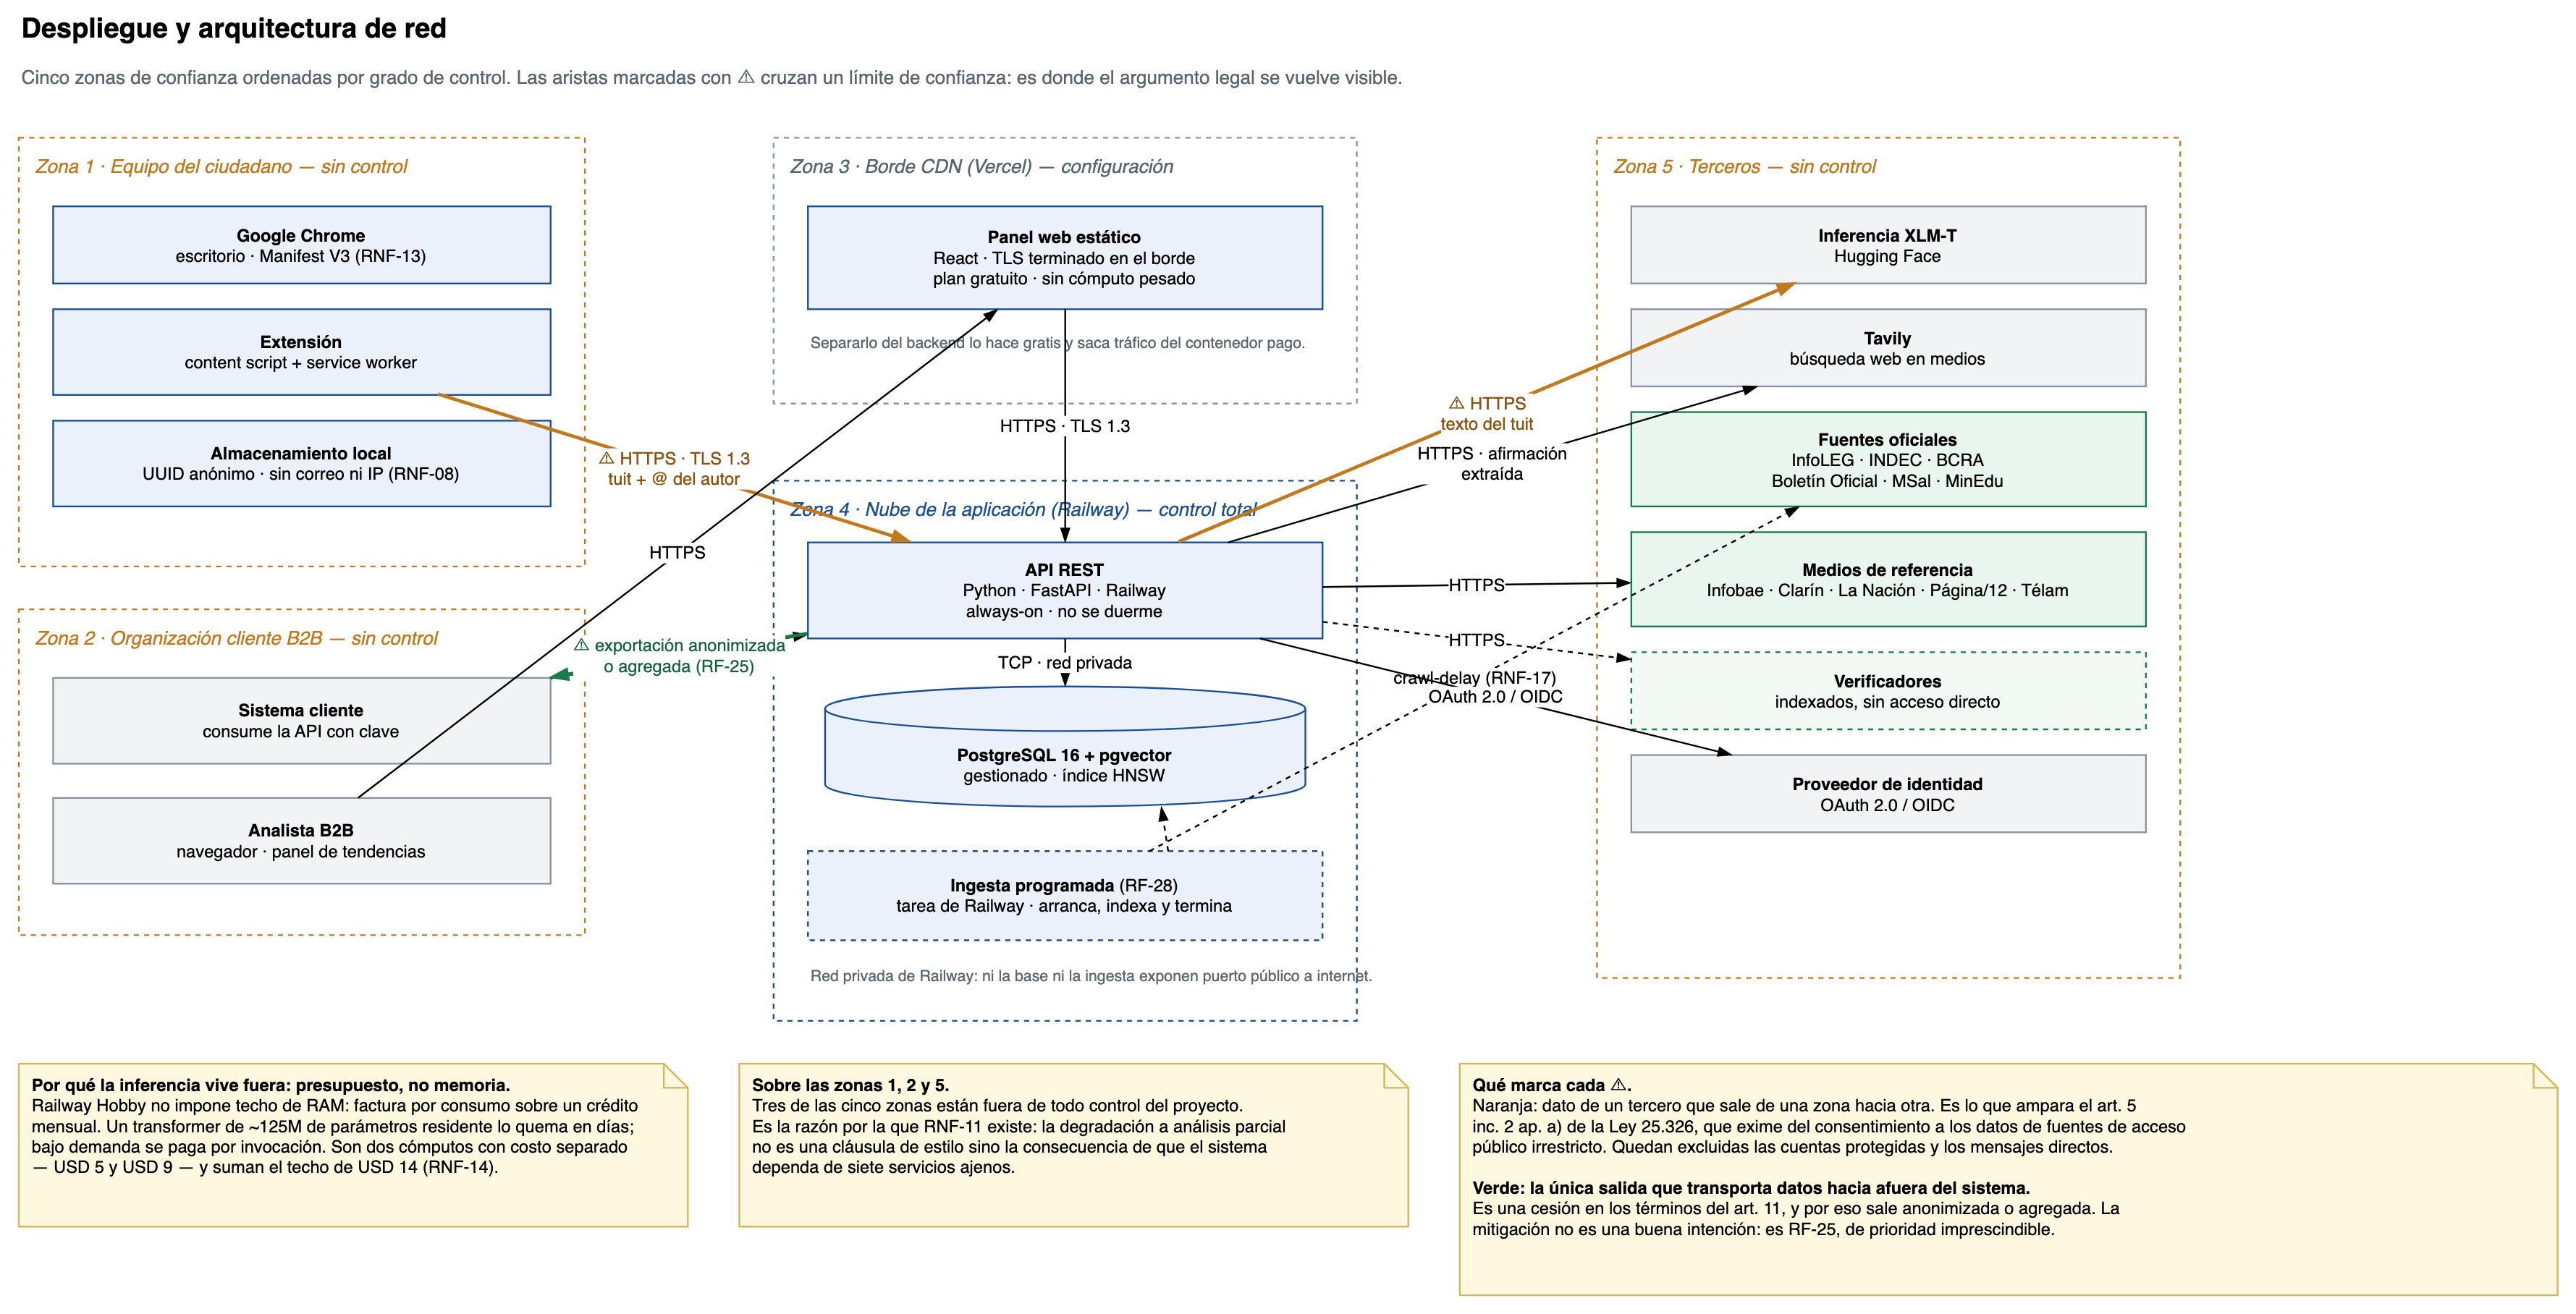
\includegraphics[width=0.95\linewidth]{chapters/figures/despliegue-red}
  \caption{Despliegue y arquitectura de red. Las cinco zonas están ordenadas por grado de control y las aristas señaladas indican los cruces de frontera de confianza. Fuente: elaboración propia.}
  \label{fig:despliegue}
\end{figure}
\end{landscape}

\section{Validación del sistema}
\label{sec:validacion}

En esta sección se describen las pruebas con las que se verifica que el sistema cumple los requerimientos enunciados en la Sección~\ref{sec:requerimientos}. La validación abarca tanto el comportamiento funcional del prototipo como el desempeño del clasificador y la experiencia de uso de un público sin conocimiento técnico.

Las pruebas se organizan en cuatro etapas. En primer lugar, se ejecutan pruebas funcionales de integración, una por cada caso de uso, complementadas por las baterías de pruebas automatizadas del servicio y de la extensión. En segundo lugar, se evalúa el clasificador sobre una partición de datos que preserva un conjunto de prueba de reserva, con métricas y modelos de contraste fijados de antemano. A continuación, se miden los requerimientos no funcionales que establecen un umbral cuantificado. Finalmente, se realiza una prueba de usabilidad con participantes sin conocimiento técnico sobre la extensión instalada. La sección cierra con una síntesis de los resultados obtenidos.

\subsection{Pruebas funcionales de integración}
\label{sec:pruebas-funcionales}

Las pruebas funcionales verifican que los módulos del sistema operen de manera integrada, desde la lectura de la publicación en la línea de tiempo hasta la presentación del veredicto y de su evidencia. Se clasifican como pruebas de integración funcional porque ejercitan la interacción entre la extensión, el servicio y las fuentes externas, y no el comportamiento aislado de cada componente.

Cada caso de prueba corresponde a un caso de uso de la Tabla~\ref{tab:trazabilidad-cu} y contrasta el resultado obtenido con la postcondición de su ficha en el Anexo~\ref{anexo:casos-uso}. Los siete casos cubren quince de los dieciséis requerimientos funcionales. RF-12, que carece de caso de uso por tratarse de un requerimiento de superficie, se verifica por inspección de la extensión y del panel web. A continuación se presentan los casos de prueba con sus resultados esperados y reales.

\subsubsection{Caso de prueba 1: Análisis automático de la línea de tiempo}

Este caso verifica que la extensión detecte las publicaciones que ingresan en el área visible, obtenga su clasificación de texto y superponga el indicador sobre cada una sin intervención del usuario.

\begin{small}
\begin{longtable}{@{}p{3.4cm} p{11.8cm}@{}}
  \caption{Caso de prueba 1: análisis automático de la línea de tiempo. Fuente: elaboración propia.}
  \label{tab:cp-01} \\
    \hline
    \textbf{Objetivo} & Verificar que la extensión identifique las publicaciones visibles, obtenga su clasificación de texto y superponga sobre cada una el indicador con su estado. \\
    \textbf{Requerimientos cubiertos} & RF-01, RF-02, RF-06, RF-07, RF-08, RF-16 \\
    \textbf{Precondiciones} & Extensión instalada y activa en Google Chrome. Servicio en funcionamiento. Sesión iniciada en X. \\
    \textbf{Entradas} & Línea de tiempo con publicaciones de texto sin análisis previo y al menos una publicación con un análisis completo vigente. \\
    \textbf{Pasos} & 1.~Abrir la línea de tiempo de X.\newline 2.~Desplazarla hasta que nuevas publicaciones ingresen en el área visible.\newline 3.~Observar el indicador de cada publicación.\newline 4.~Recargar la página y repetir el recorrido. \\
    \textbf{Resultado esperado} & Cada publicación con texto muestra el indicador en el estado \emph{sin contraste externo}. La publicación con análisis vigente muestra su nivel de veredicto sin una nueva clasificación. El resultado de cada publicación queda registrado. \\
    \textbf{Resultado real} & \Martin[inline]{Pendiente: registrar lo observado al ejecutar el caso.} \\
    \textbf{Resultado de la prueba} & \Martin[inline]{Pendiente.} \\
    \hline
\end{longtable}
\end{small}

\subsubsection{Caso de prueba 2: Análisis profundo de una publicación}

El segundo caso examina el flujo a demanda, en el que el sistema evalúa las señales de la cuenta, extrae la afirmación verificable, la contrasta con las fuentes y emite el veredicto con su justificación enlazada.

\begin{small}
\begin{longtable}{@{}p{3.4cm} p{11.8cm}@{}}
  \caption{Caso de prueba 2: análisis profundo de una publicación. Fuente: elaboración propia.}
  \label{tab:cp-02} \\
    \hline
    \textbf{Objetivo} & Verificar que, a solicitud del usuario, el sistema combine los tres puntajes parciales en un veredicto acompañado de una justificación con el enlace de cada fuente. \\
    \textbf{Requerimientos cubiertos} & RF-03, RF-04, RF-05, RF-06, RF-08, RF-09, RF-16 \\
    \textbf{Precondiciones} & Publicación con indicador visible producto del caso de prueba 1. Servicio con acceso a las fuentes oficiales indexadas y al servicio de búsqueda. \\
    \textbf{Entradas} & Publicación que contiene una afirmación verificable cubierta por una fuente oficial indexada. \\
    \textbf{Pasos} & 1.~Seleccionar el indicador de la publicación.\newline 2.~Observar el estado transitorio.\newline 3.~Esperar la actualización del indicador.\newline 4.~Abrir el detalle del análisis. \\
    \textbf{Resultado esperado} & El indicador pasa por el estado transitorio y presenta uno de los tres niveles de veredicto. El detalle muestra el desglose de los tres puntajes parciales y la justificación con el enlace de cada fuente. El análisis queda persistido con su evidencia y la versión de modelo que lo produjo. \\
    \textbf{Resultado real} & \Martin[inline]{Pendiente: registrar lo observado al ejecutar el caso.} \\
    \textbf{Resultado de la prueba} & \Martin[inline]{Pendiente.} \\
    \hline
\end{longtable}
\end{small}

\subsubsection{Caso de prueba 3: Consulta de la evidencia de un veredicto}

Este caso verifica que el usuario pueda conocer qué fuentes sostienen el veredicto, con qué postura, y acceder al documento original de cada una.

\begin{small}
\begin{longtable}{@{}p{3.4cm} p{11.8cm}@{}}
  \caption{Caso de prueba 3: consulta de la evidencia de un veredicto. Fuente: elaboración propia.}
  \label{tab:cp-03} \\
    \hline
    \textbf{Objetivo} & Verificar que el panel de evidencia presente la afirmación extraída y las fuentes vinculadas, agrupadas por tipo y por postura, cada una con un enlace funcional. \\
    \textbf{Requerimientos cubiertos} & RF-09 \\
    \textbf{Precondiciones} & Análisis completo producto del caso de prueba 2, con al menos una fuente vinculada. \\
    \textbf{Entradas} & Selección del panel de evidencia desde el detalle del análisis. \\
    \textbf{Pasos} & 1.~Abrir el panel de evidencia.\newline 2.~Revisar la afirmación extraída y las fuentes listadas.\newline 3.~Abrir el enlace de una fuente. \\
    \textbf{Resultado esperado} & El panel muestra la afirmación y las fuentes agrupadas por tipo y por postura. El enlace abre el documento original de la fuente. \\
    \textbf{Resultado real} & \Martin[inline]{Pendiente: registrar lo observado al ejecutar el caso.} \\
    \textbf{Resultado de la prueba} & \Martin[inline]{Pendiente.} \\
    \hline
\end{longtable}
\end{small}

\subsubsection{Caso de prueba 4: Informe de un veredicto incorrecto}

El cuarto caso verifica el registro de los desacuerdos del usuario, que alimentan la revisión de errores y el reentrenamiento del modelo.

\begin{small}
\begin{longtable}{@{}p{3.4cm} p{11.8cm}@{}}
  \caption{Caso de prueba 4: informe de un veredicto incorrecto. Fuente: elaboración propia.}
  \label{tab:cp-04} \\
    \hline
    \textbf{Objetivo} & Verificar que el informe de un veredicto incorrecto quede registrado y asociado al análisis, al identificador anónimo y a la versión de modelo vigente. \\
    \textbf{Requerimientos cubiertos} & RF-11 \\
    \textbf{Precondiciones} & Análisis visible en el detalle de una publicación. \\
    \textbf{Entradas} & Tipo de error (falso positivo) y motivo en texto libre. \\
    \textbf{Pasos} & 1.~Seleccionar la opción de informar el resultado.\newline 2.~Indicar el tipo de error.\newline 3.~Escribir el motivo.\newline 4.~Enviar el informe. \\
    \textbf{Resultado esperado} & El sistema confirma la recepción. El informe queda registrado con el análisis, el identificador anónimo y la versión de modelo vigente. \\
    \textbf{Resultado real} & \Martin[inline]{Pendiente: registrar lo observado al ejecutar el caso.} \\
    \textbf{Resultado de la prueba} & \Martin[inline]{Pendiente.} \\
    \hline
\end{longtable}
\end{small}

\subsubsection{Caso de prueba 5: Consulta del histórico personal}

Este caso verifica que el panel web presente los análisis solicitados desde la instalación de la extensión, asociados al navegador y no a una persona.

\begin{small}
\begin{longtable}{@{}p{3.4cm} p{11.8cm}@{}}
  \caption{Caso de prueba 5: consulta del histórico personal. Fuente: elaboración propia.}
  \label{tab:cp-05} \\
    \hline
    \textbf{Objetivo} & Verificar que el panel web liste los análisis asociados al identificador local de la extensión y permita acceder al detalle de cada uno. \\
    \textbf{Requerimientos cubiertos} & RF-10 \\
    \textbf{Precondiciones} & Al menos un análisis solicitado desde la instalación de la extensión. \\
    \textbf{Entradas} & Identificador generado localmente por la extensión. \\
    \textbf{Pasos} & 1.~Abrir el panel web desde la extensión.\newline 2.~Revisar el listado de análisis.\newline 3.~Abrir uno de los análisis listados. \\
    \textbf{Resultado esperado} & El panel presenta los análisis ordenados por fecha, cada uno con su veredicto. El análisis abierto muestra su detalle y su evidencia. \\
    \textbf{Resultado real} & \Martin[inline]{Pendiente: registrar lo observado al ejecutar el caso.} \\
    \textbf{Resultado de la prueba} & \Martin[inline]{Pendiente.} \\
    \hline
\end{longtable}
\end{small}

\subsubsection{Caso de prueba 6: Consumo de la API}

El sexto caso examina el acceso de un sistema cliente a la interfaz de clasificación autenticada, junto con el control de la clave y de la cuota.

\begin{small}
\begin{longtable}{@{}p{3.4cm} p{11.8cm}@{}}
  \caption{Caso de prueba 6: consumo de la API. Fuente: elaboración propia.}
  \label{tab:cp-06} \\
    \hline
    \textbf{Objetivo} & Verificar que la interfaz de clasificación devuelva el análisis completo ante una clave válida, registre el consumo y rechace una clave revocada. \\
    \textbf{Requerimientos cubiertos} & RF-13, RF-15 \\
    \textbf{Precondiciones} & Organización cliente dada de alta por el administrador del sistema, con una clave activa, una clave revocada y cuota disponible. \\
    \textbf{Entradas} & Texto con una afirmación verificable, enviado primero con la clave activa y luego con la clave revocada. \\
    \textbf{Pasos} & 1.~Enviar el texto con la clave activa.\newline 2.~Revisar la respuesta recibida.\newline 3.~Consultar el consumo registrado de la organización.\newline 4.~Enviar el mismo texto con la clave revocada. \\
    \textbf{Resultado esperado} & La primera solicitud devuelve el puntaje, el veredicto, la justificación y las fuentes, sin la identidad de la cuenta autora en claro, y el consumo queda registrado contra la cuota. La segunda solicitud se rechaza. \\
    \textbf{Resultado real} & \Martin[inline]{Pendiente: registrar lo observado al ejecutar el caso.} \\
    \textbf{Resultado de la prueba} & \Martin[inline]{Pendiente.} \\
    \hline
\end{longtable}
\end{small}

\subsubsection{Caso de prueba 7: Consulta del panel de tendencias}

El último caso verifica la vista que se ofrece a las organizaciones cliente, en la que ninguna cuenta autora debe aparecer identificada en claro.

\begin{small}
\begin{longtable}{@{}p{3.4cm} p{11.8cm}@{}}
  \caption{Caso de prueba 7: consulta del panel de tendencias. Fuente: elaboración propia.}
  \label{tab:cp-07} \\
    \hline
    \textbf{Objetivo} & Verificar que el analista, autenticado con la clave de su organización, consulte los temas de mayor circulación y su evolución, y exporte un recorte sin la identidad de las cuentas autoras en claro. \\
    \textbf{Requerimientos cubiertos} & RF-13, RF-14, RF-15 \\
    \textbf{Precondiciones} & Organización cliente con una clave activa y cuota disponible. Análisis acumulados en el período consultado. \\
    \textbf{Entradas} & Clave de la organización y período de consulta. \\
    \textbf{Pasos} & 1.~Autenticarse con la clave de la organización.\newline 2.~Seleccionar el período.\newline 3.~Revisar los temas, su evolución temporal y las cuentas de mayor volumen.\newline 4.~Exportar el recorte. \\
    \textbf{Resultado esperado} & El panel presenta los temas, su evolución y las cuentas de mayor volumen bajo seudónimo. El recorte exportado es agregado o tiene la cuenta autora anonimizada. \\
    \textbf{Resultado real} & \Martin[inline]{Pendiente: registrar lo observado al ejecutar el caso.} \\
    \textbf{Resultado de la prueba} & \Martin[inline]{Pendiente.} \\
    \hline
\end{longtable}
\end{small}

\subsection{Pruebas automatizadas}
\label{sec:pruebas-automatizadas}

Las pruebas funcionales se complementan con dos baterías automatizadas que se ejecutan sobre el código del prototipo sin acceso a la red ni a credenciales. En el servicio, el puerto hacia el proveedor del modelo de lenguaje se sustituye por un doble mediante el mecanismo de inyección de dependencias del \textit{framework}, lo que permite simular tanto las respuestas esperadas como la caída de cada etapa del análisis.

La batería del servicio reúne 98 pruebas y alcanza una cobertura del 92~\% de las sentencias del código de la aplicación. Ejercita, entre otros aspectos, la invariante por la cual ningún puntaje produce un nivel de veredicto sin una fuente enlazable (RNF-06), la validación de los dominios admisibles como medios de referencia frente a direcciones que los imitan, el cálculo del nivel a partir de los puntajes parciales y la devolución de un análisis parcial identificado como tal ante la falla de cualquier etapa (RNF-11). Asimismo, recorre los casos de prueba 6 y 7 tal como están escritos y verifica el registro de los informes de error y del histórico por instalación (RF-10 y RF-11), el control de la clave y de la cuota (RF-13) y la ausencia de la cuenta autora en claro en las respuestas y en la exportación (RF-15).

La batería de la extensión reúne 16 pruebas activas. Verifican que el indicador nunca permanezca en el estado transitorio ante una falla o una demora de la respuesta, que el análisis parcial se señale de forma explícita (RF-08), que los enlaces a las fuentes abran el documento original (RNF-06) y que la lectura de la estructura de la página tolere publicaciones con campos ausentes o con una forma inesperada sin interrumpir la extensión. La cobertura de esta batería no se mide.

\Martin[inline]{Si se mide la cobertura de la extensión, reemplazar la última oración por el valor.}

\subsection{Evaluación del clasificador}
\label{sec:evaluacion-clasificador}

La evaluación del clasificador se define antes de obtener cualquier resultado, para que la elección de los datos y de las métricas no dependa de los valores observados. A continuación se describen la partición de los datos, las métricas, la línea base y los modelos de contraste, y el control de calidad de las etiquetas del conjunto de prueba real.

\subsubsection{Partición de los datos}

La evaluación se apoya en cuatro conjuntos de datos con funciones diferenciadas. El conjunto de entrenamiento corresponde a la partición de entrenamiento del \textit{Spanish Fake News Corpus}, precedida por LIAR y FakeNewsNet en la variante de XLM-T que incluye la etapa en inglés. El conjunto de validación, tomado del mismo corpus, se destina a la selección de hiperparámetros, al criterio de detención del ajuste y a la elección del modelo que se sirve. El conjunto de prueba académico emplea la partición oficial de prueba del \textit{Spanish Fake News Corpus}, lo que permite comparar los resultados con los reportados en la literatura. El conjunto de prueba real corresponde al corpus argentino descrito en la Sección~\ref{sec:datos}.

Cuatro reglas gobiernan el procedimiento. La primera establece que el conjunto de prueba real opera como reserva estricta: no interviene en el ajuste de parámetros, en la selección de hiperparámetros ni en la elección del modelo, y se evalúa una única vez al término del proceso. La segunda impone respetar las particiones oficiales de los conjuntos públicos allí donde existan, condición necesaria para que los valores obtenidos resulten comparables. La tercera exige estratificación por clase y una semilla fija en toda partición propia: con 971 muestras, una partición aleatoria puede alterar la proporción entre clases lo suficiente como para desplazar la métrica, y la semilla vuelve reproducible cualquier corrida. La cuarta prohíbe la presencia de una misma publicación en más de un subconjunto, empleando como clave de eliminación de duplicados el identificador de origen cuando existe y el texto normalizado cuando no. Las particiones resultantes se conservan en archivos versionados, de modo que todos los modelos se evalúan sobre exactamente los mismos ejemplos.

\subsubsection{Métricas de evaluación}

La métrica principal es el valor F1 macro. La elección responde a la distribución de las clases y no a una convención: los conjuntos disponibles presentan proporciones desiguales entre \textit{verdadero} y \textit{falso}, y un clasificador que favoreciera de forma sistemática a la clase mayoritaria podría alcanzar una exactitud global elevada sin detectar el contenido falso, que es el caso de interés. El F1 macro promedia el desempeño de ambas clases sin ponderar por frecuencia, con lo que penaliza ese comportamiento, y conserva además su significado entre conjuntos de prueba con proporciones distintas, como la partición académica y el corpus argentino, construido cerca de la paridad.

Tres métricas complementan la evaluación. La precisión y la cobertura calculadas por clase permiten localizar el tipo de error: un falso positivo, es decir, contenido verdadero clasificado como \textit{falso}, acarrea un costo reputacional y legal superior al de un falso negativo, según se desprende del análisis de la Sección~\ref{sec:legal}. El área bajo la curva característica operativa, calculada sobre la probabilidad de la clase \textit{falso}, es independiente del umbral de decisión y habilita la comparación entre modelos sin fijar previamente un punto de corte. La matriz de confusión, por último, separa los dos tipos de error en valores absolutos y sostiene el análisis de errores con ejemplos, que indica en qué clase de publicaciones falla el modelo. La situación en que no existe evidencia para pronunciarse queda fuera de estas métricas, dado que no es una salida del clasificador sino del ensamblado, según se expuso en la Sección~\ref{sec:datos}.

\subsubsection{Línea base y modelos de contraste}

La comparación abarca cinco modelos. La línea base se construye con una representación de frecuencia de términos ponderada por frecuencia inversa de documento y un clasificador de regresión logística, y su función es establecer el desempeño alcanzable sin recurrir a modelos neuronales. Tres modelos basados en la arquitectura \textit{Transformer} se ajustan sobre los mismos datos: XLM-T \parencite{BarbieriEtAl2022}, multilingüe y pre-entrenado sobre publicaciones de la red social, que se evalúa con la etapa previa en inglés y sin ella; RoBERTuito \parencite{PerezEtAl2022}, monolingüe en español y adaptado al registro de las redes sociales, que se ajusta con su propio preprocesamiento; y BETO \parencite{CañeteEtAl2020}, monolingüe en español y pre-entrenado sobre texto formal. El contraste entre los tres permite cuantificar el costo o el beneficio de un modelo multilingüe frente a uno monolingüe.

El quinto modelo es un LLM operando sin ejemplos previos (\textit{zero-shot}), incorporado a partir de la recomendación registrada en la Sección~\ref{sec:entrevistas}. Su función es establecer el costo de oportunidad de la decisión de arquitectura, no competir en desempeño: si un modelo de propósito general alcanzara un valor F1 comparable sin requerir ajuste fino ni corpus anotado, la justificación del enfoque adoptado debería revisarse. La comparación contempla, además del desempeño, la latencia y el costo por consulta, dado que ambos condicionan la viabilidad de un servicio gratuito según se desarrolla en la Sección~\ref{sec:tecnologias}.

El modelo que se sirve en el primer módulo se elige por su valor F1 macro sobre la partición de validación del \textit{Spanish Fake News Corpus}, y nunca a partir de su desempeño sobre el corpus argentino, que de otro modo dejaría de ser una reserva estricta. Ante un empate, se prefiere el modelo de menor latencia de inferencia. Cada corrida registra sus hiperparámetros, las curvas de pérdida y las métricas por época, de manera que el proceso de entrenamiento resulte reproducible y auditable.

El requerimiento RNF-05 fija dos condiciones simultáneas sobre el veredicto del sistema: un valor F1 macro de 0,75 y un desempeño superior al de la línea base sobre el mismo conjunto. Ambas cumplen funciones distintas. El umbral absoluto acota el desempeño mínimo aceptable para un servicio que emite veredictos, y la comparación con la línea base exige que el modelo aporte respecto de una alternativa sin redes neuronales.

La versión inicial del requerimiento fijaba un valor de 0,80 y una mejora de diez puntos porcentuales, tomados de los resultados que la literatura reporta sobre particiones de validación del \textit{Spanish Fake News Corpus}. La meta se recalibró después de evaluar los modelos sobre la partición de prueba de ese corpus y antes de evaluar el conjunto de prueba real, que de ese modo conserva su condición de reserva estricta. La partición de prueba introduce de manera deliberada noticias de otra temática y de otros países hispanohablantes, y el mejor sistema de la tarea compartida que la presentó obtuvo sobre ella un valor F1 macro de 0,7666 \parencite{GomezAdornoEtAl2021}. Un umbral de 0,80 exigía, por lo tanto, superar el mejor resultado publicado sobre un conjunto con desplazamiento de dominio, lo que no constituía un criterio de aceptación sino una meta de investigación. El valor de 0,75 se ubica en el rango de los mejores sistemas de esa tarea compartida.

Una segunda revisión cambió el objeto de la medición, no el umbral. La versión anterior exigía el valor al clasificador, y la Sección~\ref{sec:resultados-argentino} muestra que ningún clasificador de texto lo alcanza sobre publicaciones breves. El sistema, sin embargo, no emite su veredicto a partir del clasificador: lo combina con el contraste contra fuentes y no lo emite sin una fuente enlazable (RNF-06). Se reformuló RNF-05 para medir lo que el usuario recibe, que es el veredicto del sistema completo, y la revisión se realizó antes de ejecutar el sistema sobre el conjunto de prueba real. La correspondencia con las dos clases se fijó en el mismo momento: los niveles \enquote{contradicho por fuentes oficiales} e \enquote{información sospechosa} equivalen a \textit{falso}, el nivel \enquote{parece verificado} a \textit{verdadero}, y el estado sin contraste externo, así como la ausencia de una afirmación verificable, se computan como error en ambas clases, de modo que abstenerse no mejora el valor F1. La línea base de referencia es la mejor de las dos evaluadas sobre el mismo conjunto.

\subsubsection{Calidad de las etiquetas}

El conjunto de prueba real no se anota a partir del juicio propio sobre cada publicación. La etiqueta se toma de una verificación ya publicada por Chequeado o de la fuente oficial que la publicación cita, y el anotador se limita a trasladarla al esquema de dos clases. Una guía de etiquetado fija la correspondencia entre cada calificación del verificador y las dos clases, junto con los casos que se descartan por no admitir una asignación inequívoca. La anotación la realiza un único anotador, el autor del trabajo, que revisa y confirma cada fila de una planilla de candidatos en la que figuran el enlace a la publicación, su texto, la calificación original o el dato oficial citado, el enlace a la nota o al documento que la sustenta y la etiqueta propuesta.

El procedimiento no incluye una medición del acuerdo entre anotadores, y la decisión se declara como tal. La subjetividad que esa medición controla se desplaza hacia la fuente: la calificación la emitió una organización de verificación con metodología pública, o la comprueba un documento oficial, y el corpus conserva para cada publicación el enlace que sustenta su etiqueta, de modo que cualquier lector puede auditarla. La contrapartida es un sesgo de selección que conviene enunciar: el corpus contiene solo afirmaciones que alguien ya verificó o que citan un dato oficial, y no necesariamente representa la totalidad de lo que circula en la red social.

\subsubsection{Resultados sobre el conjunto de prueba real}
\label{sec:resultados-argentino}

El conjunto de prueba real reúne 108 publicaciones, 48 verdaderas y 60 falsas, y se evaluó con el umbral de decisión de 0,5 que cada modelo emplea sobre el \textit{Spanish Fake News Corpus}. La evaluación sigue el protocolo descrito en esta sección: BETO, elegido por su valor F1 macro de 0,876 sobre la partición de validación de ese corpus, se evaluó una única vez, junto con la línea base. La Tabla~\ref{tab:resultados-argentino} presenta ese resultado y el de la adaptación que se describe a continuación.

\begin{table}[t]
  \centering
  \small
  \caption{Valor F1 macro y área bajo la curva ROC sobre el conjunto de prueba real (108 publicaciones), con el intervalo de confianza del 95~\% del valor F1 estimado por remuestreo (5000 réplicas). En el sistema completo, el área se calcula sobre el puntaje final y el valor F1 computa como error las publicaciones sin veredicto. Fuente: elaboración propia.}
  \label{tab:resultados-argentino}
  \begin{tabular}{@{}l l c c c@{}}
    \hline
    \textbf{Modelo} & \textbf{Entrenamiento} & \textbf{F1 macro} & \textbf{IC 95~\%} & \textbf{AUC-ROC} \\
    \hline
    Línea base & \textit{Spanish Fake News Corpus} & 0,496 & 0,40--0,59 & 0,604 \\
    BETO & \textit{Spanish Fake News Corpus} & 0,439 & 0,35--0,53 & 0,551 \\
    \hline
    Línea base & Ídem, más afirmaciones de Chequeado & 0,527 & 0,43--0,62 & 0,585 \\
    BETO & Ídem, más afirmaciones de Chequeado & 0,540 & 0,44--0,64 & 0,578 \\
    \hline
    Sistema completo & BETO adaptado, contraste con fuentes y combinador & 0,654 & 0,56--0,74 & 0,739 \\
    \hline
  \end{tabular}
\end{table}

Los dos modelos del protocolo original se ubicaron en el nivel del azar y clasificaron como falsa la mayor parte de las publicaciones: BETO asignó esa clase a 91 de las 108. El mismo código de inferencia reproduce el valor de 0,760 sobre la partición de prueba del \textit{Spanish Fake News Corpus}, lo que descarta un error de implementación y señala como causa el desplazamiento de dominio. Los modelos se ajustaron sobre noticias completas, con una mediana cercana a los quinientos \textit{tokens}, y se evaluaron sobre publicaciones de pocas líneas, en otro registro y sobre otros temas. El corpus argentino se diseñó precisamente para medir esa distancia, y el resultado indica que el rendimiento sobre un corpus académico no se traslada a la red social.

A partir de ese diagnóstico se realizó una adaptación posterior, que se declara como tal porque se decidió después de conocer el resultado sobre el conjunto de prueba real. Se construyó un conjunto de entrenamiento con 2107 afirmaciones calificadas por Chequeado, 965 verdaderas y 1142 falsas, tomadas del título de cada nota y llevadas a dos clases con la misma guía de etiquetado del corpus de prueba. De cada título se conserva solo la afirmación: se eliminan las fórmulas del verificador que anticipan la etiqueta, como \enquote{Es falso que}, y se descartan los títulos que califican la atribución de una cita y no su contenido. Se excluyeron las notas de las que provienen las publicaciones de prueba y toda afirmación que compartiera el 60~\% o más de sus palabras con alguna de ellas, condición que verifica una prueba automatizada. El conjunto se dividió en entrenamiento y validación en proporción 85/15, con estratificación por clase. BETO continuó su ajuste sobre esas afirmaciones a partir del modelo entrenado con el \textit{Spanish Fake News Corpus}, con la época elegida por el valor F1 macro sobre la validación de Chequeado (0,702), y la línea base se reentrenó sobre la unión de ambos conjuntos de entrenamiento (0,650 sobre la misma validación).

La adaptación mejoró a BETO en diez puntos sobre el conjunto de prueba real, y el remuestreo pareado ubica esa mejora por encima de cero con un 97,6~\% de las réplicas. Sin embargo, el valor alcanzado, 0,540, queda lejos del umbral de 0,75, y la ventaja de 1,3 puntos sobre la línea base adaptada no se distingue del ruido de muestreo: con 108 publicaciones, el intervalo de esa diferencia va de $-0{,}11$ a $+0{,}14$. El clasificador, por sí solo, no alcanza ninguna de las dos condiciones de RNF-05. La curva de entrenamiento de la última etapa muestra, además, que la pérdida de validación crece desde la segunda época mientras el valor F1 se mantiene estable, señal de un modelo cada vez más confiado en sus errores. El resultado sugiere que la detección sobre publicaciones breves requiere un volumen de ejemplos del propio dominio mayor que el que ofrece un verificador, y respalda la decisión de arquitectura de no emitir un veredicto a partir del clasificador sin el respaldo de fuentes enlazables que establece RNF-06.

El sistema completo, que es el objeto de RNF-05 tras su reformulación, se ejecutó una única vez sobre las 108 publicaciones, con el clasificador adaptado como primer módulo y la configuración de pesos vigente. Emitió un veredicto en 105 de ellas, el 97~\% del conjunto, y alcanzó un valor F1 macro de 0,654, con un intervalo de confianza del 95~\% entre 0,56 y 0,74. El resultado supera con claridad a la línea base, cuyo valor de 0,527 queda por debajo del extremo inferior del intervalo, y mejora en once puntos al clasificador aislado. No alcanza, en cambio, el umbral de 0,75, que tampoco queda contenido en el intervalo, por lo que RNF-05 se cumple en su segunda condición y no en la primera. El contraste con fuentes aporta, en consecuencia, la mayor parte de la capacidad de discriminación del sistema, en línea con la hipótesis que motivó la arquitectura.

El error se concentra en las publicaciones verdaderas: el sistema asignó a 23 de las 48 uno de los dos niveles desfavorables, mientras que solo 11 de las 60 falsas recibieron el nivel de verificación favorable. Una explicación posible, que esta evaluación no permite aislar, es el desfase temporal entre la publicación y el análisis: 78 de las 108 publicaciones, el 72~\%, son anteriores a 2022, y la búsqueda recupera la información disponible en 2026, de modo que una cifra correcta al momento de publicarse puede aparecer contradicha por datos posteriores. El sistema está concebido para publicaciones recientes, y esa condición no se reproduce en el conjunto de prueba. En sentido contrario opera un sesgo que favorece al sistema: Chequeado integra el escalón de verificaciones previas y figuró entre las fuentes recuperadas en 87 de los 108 análisis, con lo que la búsqueda pudo encontrar la misma nota que asignó la etiqueta. El resultado describe el desempeño sobre contenido que ya fue verificado y sobreestima, en esa medida, el desempeño ante desinformación nueva. Para el clasificador aislado queda abierta una línea de trabajo que no se ensayó: reescribir las afirmaciones de entrenamiento con el registro de una publicación en la red social mediante un LLM, conservando su etiqueta, para reducir la distancia entre los títulos del verificador y las publicaciones que el sistema analiza.

\subsection{Mediciones de los requerimientos no funcionales}
\label{sec:mediciones-rnf}

Los requerimientos no funcionales que establecen un umbral cuantificado se verifican mediante una medición sobre el prototipo en funcionamiento o sobre el conjunto de prueba real. La Tabla~\ref{tab:criterios-validacion} enumera cada uno con su umbral, el procedimiento de medición y el valor obtenido. Un requerimiento se considera cumplido cuando el valor medido no supera el umbral, en el caso de los tiempos y del costo, o lo alcanza, en el caso de la calidad del modelo.

\begin{table}[t]
  \centering
  \small
  \caption{Mediciones de los requerimientos no funcionales con umbral cuantificado. Fuente: elaboración propia.}
  \label{tab:criterios-validacion}
  \begin{tabular}{@{}l p{3cm} p{6.1cm} p{3.6cm}@{}}
    \hline
    \textbf{Req.} & \textbf{Umbral} & \textbf{Procedimiento de medición} & \textbf{Valor medido} \\
    \hline
    RNF-01 & 2 s, percentil 95 & Instrumentación de la extensión y medición sobre una sesión de navegación real & \Martin[inline]{Pendiente.} \\
    RNF-02 & 8 s, percentil 95 & Registro de traza del servicio, medido de extremo a extremo & \Martin[inline]{Pendiente.} \\
    RNF-03 & 300 ms & Prueba de carga sobre publicaciones previamente analizadas y vigentes & \Martin[inline]{Pendiente.} \\
    RNF-04 & 50 ms & Perfilador de rendimiento del navegador sobre el hilo principal & \Martin[inline]{Pendiente.} \\
    RNF-05 & F1 macro 0,75 del veredicto y superior a la línea base & Ejecución del sistema completo sobre el conjunto de prueba real & 0,654 (IC 0,56--0,74); línea base 0,527. Supera a la línea base y no alcanza 0,75: no se cumple \\
    RNF-12 & HTTPS y claves resumidas & Inspección del tráfico y del esquema de la base de datos & \Martin[inline]{Pendiente.} \\
    RNF-13 & Chrome bajo Manifest V3 en tres sistemas operativos & Ejecución manual de la matriz de compatibilidad & \Martin[inline]{Pendiente.} \\
    RNF-14 & 14 dólares mensuales & Panel de facturación de los proveedores de infraestructura & \Martin[inline]{Pendiente.} \\
    \hline
  \end{tabular}
\end{table}

Entre los requerimientos no funcionales que expresan una condición cualitativa y no un umbral, RNF-06 y RNF-11 se verifican mediante las pruebas automatizadas descritas en la Sección~\ref{sec:pruebas-automatizadas}, y RNF-15, que exige que el indicador resulte interpretable sin instrucción previa, mediante la prueba de usabilidad que se presenta a continuación.

\subsection{Prueba de usabilidad}
\label{sec:usabilidad}

La prueba de usabilidad evalúa si un usuario sin conocimiento técnico interpreta el indicador y completa el análisis de una publicación sin instrucción previa, condición que establece RNF-15. Participan personas que no intervinieron en el desarrollo y que no conocen el funcionamiento interno del sistema.

\Martin[inline]{Completar la cantidad de participantes, su perfil, la fecha y el lugar de la prueba.}

Cada participante utiliza la extensión instalada sobre su propia sesión de X, o sobre una cuenta de prueba, en Google Chrome de escritorio. No recibe explicación alguna sobre el significado del indicador. Se le solicitan tres tareas, que corresponden a los tres casos de uso del ciudadano de mayor frecuencia: interpretar el indicador de una publicación de su línea de tiempo, solicitar el análisis profundo de esa publicación y abrir una de las fuentes que sostienen el veredicto. Durante la ejecución se registra si cada tarea se completa sin ayuda y las dudas que el participante expresa en voz alta.

\Martin[inline]{Insertar aquí las fotos del uso real de la extensión durante la prueba, una figura por foto, con \texttt{[t]} y la fuente en el \emph{caption}.}

% Plantilla para cada foto de la prueba de usabilidad:
% \begin{figure}[t]
%   \centering
%   \includegraphics[width=0.8\linewidth]{chapters/figures/usabilidad-1}
%   \caption{Participante utilizando la extensión durante la prueba de usabilidad. Fuente: elaboración propia.}
%   \label{fig:usabilidad-1}
% \end{figure}

Al finalizar las tareas, cada participante responde un cuestionario cualitativo sobre su experiencia. La Tabla~\ref{tab:cuestionario-usabilidad} presenta las preguntas y una síntesis de las respuestas obtenidas.

\begin{table}[t]
  \centering
  \small
  \caption{Resultados del cuestionario cualitativo de la prueba de usabilidad. Fuente: elaboración propia.}
  \label{tab:cuestionario-usabilidad}
  \begin{tabular}{@{}p{6.4cm} p{8.8cm}@{}}
    \hline
    \textbf{Pregunta} & \textbf{Respuesta de los participantes} \\
    \hline
    ¿Qué entendiste que indicaba la marca que apareció sobre las publicaciones? & \Martin[inline]{Pendiente.} \\
    ¿Te resultó claro qué hacer para obtener más información sobre una publicación? & \Martin[inline]{Pendiente.} \\
    ¿Las fuentes que mostró el análisis te permitieron comprobar el resultado por tu cuenta? & \Martin[inline]{Pendiente.} \\
    ¿Hubo algún momento en que no supieras qué estaba haciendo la extensión? & \Martin[inline]{Pendiente.} \\
    ¿La extensión interfirió con tu forma habitual de usar X? & \Martin[inline]{Pendiente.} \\
    ¿Usarías la extensión en tu navegador? ¿Por qué? & \Martin[inline]{Pendiente.} \\
    \hline
  \end{tabular}
\end{table}

La percepción cualitativa se complementa con la escala de usabilidad del sistema (\emph{System Usability Scale}, SUS), un cuestionario de diez afirmaciones que el participante valora de 1 (totalmente en desacuerdo) a 5 (totalmente de acuerdo) \parencite{Brooke1996}. Las afirmaciones impares se formulan en sentido positivo y las pares en sentido negativo. El puntaje de cada participante se obtiene restando 1 a la valoración de cada afirmación impar, restando de 5 la valoración de cada afirmación par y multiplicando la suma por 2,5, lo que produce un valor entre 0 y 100. La Tabla~\ref{tab:sus} presenta la valoración media de cada afirmación y el puntaje resultante.

\begin{table}[t]
  \centering
  \small
  \caption{Resultados de la escala de usabilidad del sistema (SUS). Fuente: elaboración propia sobre la escala de \textcite{Brooke1996}.}
  \label{tab:sus}
  \begin{tabular}{@{}r p{9.8cm} p{4cm}@{}}
    \hline
    \textbf{N.º} & \textbf{Afirmación} & \textbf{Valoración media} \\
    \hline
    1 & Creo que me gustaría usar este sistema con frecuencia. & \Martin[inline]{Pendiente.} \\
    2 & Encontré el sistema innecesariamente complejo. & \Martin[inline]{Pendiente.} \\
    3 & Pensé que el sistema era fácil de usar. & \Martin[inline]{Pendiente.} \\
    4 & Creo que necesitaría el apoyo de una persona con conocimientos técnicos para poder usar este sistema. & \Martin[inline]{Pendiente.} \\
    5 & Encontré que las distintas funciones del sistema estaban bien integradas. & \Martin[inline]{Pendiente.} \\
    6 & Pensé que había demasiada inconsistencia en el sistema. & \Martin[inline]{Pendiente.} \\
    7 & Imagino que la mayoría de las personas aprendería a usar este sistema muy rápidamente. & \Martin[inline]{Pendiente.} \\
    8 & Encontré el sistema muy engorroso de usar. & \Martin[inline]{Pendiente.} \\
    9 & Me sentí muy seguro usando el sistema. & \Martin[inline]{Pendiente.} \\
    10 & Necesité aprender muchas cosas antes de poder empezar a usar este sistema. & \Martin[inline]{Pendiente.} \\
    \hline
    & \textbf{Puntaje SUS medio (0 a 100)} & \Martin[inline]{Pendiente.} \\
    \hline
  \end{tabular}
\end{table}

\Martin[inline]{Narrar aquí el desarrollo de la prueba: tareas completadas sin ayuda, dudas registradas y cambios en la interfaz que surgieron a partir de ellas. Definir si RNF-15 se acepta con un umbral de SUS.}

\FloatBarrier
\subsection{Síntesis de la validación}
\label{sec:sintesis-validacion}

Las pruebas funcionales de integración recorren los siete casos de uso del sistema y cubren quince de los dieciséis requerimientos funcionales, mientras que el restante, RF-12, se verifica por inspección de la interfaz. Las baterías automatizadas suman 98 pruebas en el servicio, con una cobertura del 92~\% de las sentencias, y 16 en la extensión, y aseguran las invariantes de explicabilidad y de degradación parcial que resultan difíciles de provocar de forma sistemática en una prueba manual.

\Martin[inline]{Agregar cuántos casos de prueba resultaron aprobados.}

En cuanto a la calidad del veredicto, el valor F1 macro del sistema completo sobre el conjunto de prueba real y su diferencia con la línea base determinan el cumplimiento de RNF-05. Las mediciones de rendimiento sobre el prototipo en funcionamiento establecen si los tiempos del flujo automático, del flujo a demanda y de la caché se encuentran dentro de sus umbrales.

El sistema completo obtuvo un valor F1 macro de 0,654 sobre el conjunto de prueba real, con veredicto en el 97~\% de las publicaciones: supera a la línea base y no alcanza el umbral de 0,75, por lo que RNF-05 no se cumple. Por sí solo, el clasificador queda más lejos del umbral. Sobre el conjunto de prueba real, BETO obtuvo un valor F1 macro de 0,439, por debajo de la línea base (0,496); tras la adaptación con afirmaciones de Chequeado alcanzó 0,540, frente a 0,527 de la línea base adaptada, una diferencia que no se distingue del ruido de muestreo (Sección~\ref{sec:resultados-argentino}).

\Martin[inline]{Agregar las latencias medidas en el percentil 95 y el costo mensual de la infraestructura.}

Finalmente, la prueba de usabilidad aporta la evidencia sobre la interpretación del indicador por parte de un público sin conocimiento técnico. En conjunto, estas pruebas constituyen la evidencia sobre la que se evalúa el cumplimiento de cada objetivo específico del trabajo.

\Martin[inline]{Agregar el puntaje SUS medio y los hallazgos principales de la prueba.}
